% ---------------------------------------------------------------
% TEMPLATE TCC2 - SENAC SANTO AMARO
% ---------------------------------------------------------------
% Trabalho de Conclusão de Curso 2
% ---------------------------------------------------------------

\documentclass[
    12pt,                % tamanho da fonte
    openright,           % capítulos começam em página ímpar
    oneside,             % para impressão em apenas um lado do papel
    a4paper,             % tamanho do papel
    english,             % idioma adicional
    brazil               % idioma principal
]{abntex2}

% ---------------------------------------------------------------
% PACOTES
% ---------------------------------------------------------------
\usepackage{lmodern}                % Fonte Latin Modern
\usepackage[T1]{fontenc}            % Seleção de códigos de fonte
\usepackage[utf8]{inputenc}         % Codificação do documento
\usepackage{lastpage}               % Usado pela Ficha catalográfica
\usepackage{indentfirst}            % Indenta o primeiro parágrafo
\usepackage{color}                  % Controle de cores
\usepackage{graphicx}               % Inclusão de gráficos
\usepackage{microtype}              % Melhorias de justificação
\usepackage{float}                  % Para posicionamento de figuras
\usepackage{booktabs}               % Tabelas profissionais
\usepackage{multirow}               % Células mescladas em tabelas
\usepackage{longtable}              % Tabelas longas
\usepackage{amsmath,amssymb}        % Símbolos matemáticos
\usepackage{pgfgantt}               % Diagramas de Gantt
\usepackage[brazilian,hyperpageref]{backref}  % Páginas com citações
\usepackage[alf]{abntex2cite}       % Citações ABNT
\usepackage{tabularx}               % Tabelas

% ---------------------------------------------------------------
% CONFIGURAÇÕES DO PDF
% ---------------------------------------------------------------
\makeatletter
\hypersetup{
    pdftitle={\@title},
    pdfauthor={\@author},
    pdfsubject={TCC2 - Senac Santo Amaro},
    pdfcreator={LaTeX with abnTeX2},
    pdfkeywords={tcc}{senac}{santo amaro}{trabalho de conclusão},
    colorlinks=true,        % false: links em caixas; true: links coloridos
    linkcolor=blue,         % cor dos links internos
    citecolor=blue,         % cor dos links para bibliografia
    filecolor=magenta,      % cor dos links para arquivos
    urlcolor=blue,
    bookmarksdepth=4
}
\makeatother

% ---------------------------------------------------------------
% CONFIGURAÇÕES DE APARÊNCIA DO PDF FINAL
% ---------------------------------------------------------------
\definecolor{blue}{RGB}{41,5,195}

% ---------------------------------------------------------------
% INFORMAÇÕES DO DOCUMENTO
% ---------------------------------------------------------------
\titulo{Classificação Automática de Chamados de TI Utilizando Processamento de Linguagem Natural com Explicabilidade Baseada em Grafos}
\autor{Agatha Barbosa Marinho dos Santos \\
Bruna Kinjo Luiz Pinto \\
Kayke Ahrens Biscegli}
\local{São Paulo}
\data{2026}
\orientador{Prof. Douglas José Baquião Ribeiro}
% \coorientador{Prof. Nome do Coorientador} % Descomente se houver coorientador

\instituicao{%
  Senac -- Serviço Nacional de Aprendizagem Comercial
  \par
  Unidade Santo Amaro
  \par
  Curso de Bacharelado em Ciência da Computação
}

\tipotrabalho{Trabalho de Conclusão de Curso II}

\preambulo{Trabalho de Conclusão de Curso II apresentado ao Senac Santo Amaro como requisito para conclusão do curso de Bacharelado em Ciência da Computação.}

% ---------------------------------------------------------------
% COMPILA O ÍNDICE
% ---------------------------------------------------------------
\makeindex

% ---------------------------------------------------------------
% INÍCIO DO DOCUMENTO
% ---------------------------------------------------------------
% Legenda "Fonte:" em tamanho menor que o texto (ABNT)
\let\legendoriginal\legend
\renewcommand{\legend}[1]{\legendoriginal{\small #1}}
\setlength{\emergencystretch}{3em}
\begin{document}

% Seleciona o idioma do documento
\selectlanguage{brazil}

% Retira espaço extra obsoleto entre as frases
\frenchspacing

% ---------------------------------------------------------------
% ELEMENTOS PRÉ-TEXTUAIS
% ---------------------------------------------------------------
\pretextual

% ---------------------------------------------------------------
% CAPA
% ---------------------------------------------------------------
\imprimircapa

% ---------------------------------------------------------------
% FOLHA DE ROSTO
% ---------------------------------------------------------------
\imprimirfolhaderosto

% ---------------------------------------------------------------
% RESUMO
% ---------------------------------------------------------------
\begin{resumo}
O objetivo deste trabalho é investigar como a inclusão de uma camada de explicabilidade baseada em SHAP, LIME e grafos de co-ocorrência a um \textit{pipeline} de classificação com BERTimbau contribui para a auditabilidade do processo decisório, comparando a qualidade das explicações dos dois métodos, utilizando chamados de suporte técnico em português brasileiro. A motivação é que classificadores baseados em \textit{transformers} não revelam por que atribuíram uma categoria a um chamado, o que dificulta a auditoria de suas decisões. Os dados reúnem chamados anonimizados cedidos por duas empresas do setor farmacêutico, a Empresa A e a Empresa B, em um total de 53.279 chamados em 11 categorias, divididos em treino, validação e teste de modo que textos repetidos fiquem no mesmo conjunto. Foram comparados quatro cenários, que acrescentam um componente por vez: um \textit{baseline} SVM com TF-IDF, o \textit{fine-tuning} do BERTimbau, as explicações SHAP e LIME, e o grafo de co-ocorrência ponderado por essas explicações. Em uma amostra de 98 chamados do conjunto de teste, o SHAP e o LIME foram avaliados quanto à fidelidade, à estabilidade e à concordância entre si, e a rastreabilidade do grafo, tomada como critério de auditabilidade, foi examinada em casos aplicados. O BERTimbau obteve F1-macro de 0,628 e acurácia de 0,724 no conjunto de teste. O \textit{baseline} SVM com TF-IDF obteve F1-macro de 0,591; a diferença do BERTimbau foi de 3,7 pontos percentuais (intervalo de confiança de 95\%: 1,0 a 6,7), abaixo da meta de 5 pontos estabelecida inicialmente.
Nos 98 chamados, SHAP e LIME tiveram fidelidade bem acima do acaso e apontaram a mesma palavra no topo em 69\% dos chamados; só o Tau-LOO distinguiu os métodos, a favor do LIME, e, nos chamados em que o SHAP precisou ser estimado por amostragem (2.000 consultas), ele foi mais estável que o LIME no Jaccard e no Spearman, mas menos estável na mesma palavra no topo (83\% dos pares de repetições, contra 93\% do LIME nos mesmos chamados).
Nos três casos aplicados, cada nó e cada aresta do grafo pôde ser levado ao chamado e aos pesos do SHAP e do LIME, e o grafo expôs, por exemplo, que um erro do modelo se apoiou em muito pouca evidência.
Os resultados foram integrados a uma interface \textit{web} que classifica um chamado digitado, exibe o grafo de co-ocorrência e permite alternar entre os pesos do SHAP e do LIME; a interface é uma prova de conceito e não foi avaliada junto a analistas de TI.

\vspace{\onelineskip}

\noindent
\textbf{Palavras-chave}: Processamento de Linguagem Natural. BERT. Inteligência Artificial Explicável. Grafos de Co-ocorrência. Classificação de Chamados de TI.
\end{resumo}

\begin{resumo}[Abstract]
\begin{otherlanguage*}{english}
The objective of this work is to investigate how adding an explainability layer based on SHAP, LIME and co-occurrence graphs to a BERTimbau classification \textit{pipeline} contributes to the auditability of the decision process, comparing the quality of the explanations produced by the two methods, using technical support tickets in Brazilian Portuguese. The motivation is that \textit{transformer}-based classifiers do not reveal why they assigned a category to a ticket, which makes it hard to audit their decisions. The data comprise anonymized tickets provided by two companies in the pharmaceutical sector, Company A and Company B, totaling 53,279 tickets in 11 categories, split into training, validation and test sets so that repeated texts remain in the same set. Four scenarios were compared, each adding one component: a \textit{baseline} SVM with TF-IDF, the \textit{fine-tuning} of BERTimbau, the SHAP and LIME explanations, and the co-occurrence graph weighted by those explanations. On a sample of 98 tickets from the test set, SHAP and LIME were evaluated for faithfulness, stability and agreement with each other, and the traceability of the graph, taken as the criterion of auditability, was examined in applied cases. BERTimbau achieved a macro F1 of 0.628 and an accuracy of 0.724 on the test set. The TF-IDF SVM \textit{baseline} achieved a macro F1 of 0.591; the difference in favor of BERTimbau was 3.7 percentage points (95\% confidence interval: 1.0 to 6.7), below the 5-point target set initially.
On the 98 tickets, SHAP and LIME showed faithfulness well above chance and pointed to the same top word in 69\% of tickets; only Tau-LOO separated the methods, favoring LIME, and, in the tickets where SHAP had to be estimated by sampling (2,000 queries), it was more stable than LIME in Jaccard and Spearman but less stable in the same top word (83\% of repetition pairs, versus 93\% for LIME on the same tickets).
In the three applied cases, every node and edge of the graph could be traced back to the ticket and to the SHAP and LIME weights, and the graph showed, for example, that a model error relied on very little evidence.
The results were integrated into a web interface that classifies a typed ticket, displays the co-occurrence graph and allows switching between SHAP and LIME weights; the interface is a proof of concept and was not evaluated with IT analysts.

\vspace{\onelineskip}

\noindent
\textbf{Keywords}: Natural Language Processing. BERT. Explainable Artificial Intelligence. Co-occurrence Graphs. IT Ticket Classification.
\end{otherlanguage*}
\end{resumo}

% ---------------------------------------------------------------
% LISTA DE ILUSTRAÇÕES
% ---------------------------------------------------------------
 \pdfbookmark[0]{\listfigurename}{lof}
 \listoffigures*
 \cleardoublepage

% ---------------------------------------------------------------
% LISTA DE TABELAS
% ---------------------------------------------------------------
 \pdfbookmark[0]{\listtablename}{lot}
 \listoftables*
 \cleardoublepage

% ---------------------------------------------------------------
% LISTA DE ABREVIATURAS E SIGLAS
% ---------------------------------------------------------------
\begin{siglas}
  \item[AOPC] \textit{Area Over the Perturbation Curve} (Área sobre a Curva de Perturbação)
  \item[BEGNN] \textit{BERT-Enhanced Graph Neural Network} (Rede Neural de Grafos Aprimorada por BERT)
  \item[BERT] \textit{Bidirectional Encoder Representations from Transformers} (Representações de Codificador Bidirecional a partir de Transformers)
  \item[BERTimbau] Variante do BERT pré-treinada para o português brasileiro
  \item[BiLSTM] \textit{Bidirectional Long Short-Term Memory} (Memória de Longo e Curto Prazo Bidirecional)
  \item[BrWaC] \textit{Brazilian Web as Corpus} (Web Brasileira como Corpus)
  \item[CNN] \textit{Convolutional Neural Network} (Rede Neural Convolucional)
  \item[CoT] \textit{Chain-of-Thought} (Cadeia de Raciocínio)
  \item[CPU] \textit{Central Processing Unit} (Unidade Central de Processamento)
  \item[CSS] \textit{Cascading Style Sheets} (Folhas de Estilo em Cascata)
  \item[CUDA] \textit{Compute Unified Device Architecture} (Arquitetura Unificada de Dispositivos de Computação)
  \item[E5] \textit{EmbEddings from bidirEctional Encoder rEpresentations} (\textit{Embeddings} a partir de Representações de Codificador Bidirecional)
  \item[GCN] \textit{Graph Convolutional Network} (Rede Neural Convolucional em Grafos)
  \item[GloVe] \textit{Global Vectors for Word Representation} (Vetores Globais para Representação de Palavras)
  \item[GNN] \textit{Graph Neural Network} (Rede Neural de Grafos)
  \item[GPT] \textit{Generative Pre-trained Transformer} (Transformer Generativo Pré-treinado)
  \item[GPU] \textit{Graphics Processing Unit} (Unidade de Processamento Gráfico)
  \item[HOOM] \textit{Hybrid Online Offline Model} (Modelo Híbrido \textit{Online} e \textit{Offline})
  \item[IC] Intervalo de Confiança
  \item[ITIL] \textit{Information Technology Infrastructure Library} (Biblioteca de Infraestrutura de Tecnologia da Informação)
  \item[ITSM] \textit{IT Service Management} (Gerenciamento de Serviços de TI)
  \item[JSON] \textit{JavaScript Object Notation} (Notação de Objetos JavaScript)
  \item[LGPD] Lei Geral de Proteção de Dados Pessoais
  \item[LIME] \textit{Local Interpretable Model-Agnostic Explanations} (Explicações Locais Interpretáveis Independentes de Modelo)
  \item[LLM] \textit{Large Language Model} (Modelo de Linguagem de Grande Porte)
  \item[LOO] \textit{Leave-One-Out} (Deixar Um de Fora)
  \item[LSTM] \textit{Long Short-Term Memory} (Memória de Longo e Curto Prazo)
  \item[mBERT] \textit{Multilingual BERT} (BERT Multilíngue)
  \item[MLM] \textit{Masked Language Modeling} (Modelagem de Linguagem com Máscara)
  \item[MLP] \textit{Multilayer Perceptron} (Perceptron Multicamadas)
  \item[NER] \textit{Named Entity Recognition} (Reconhecimento de Entidades Nomeadas)
  \item[NLTK] \textit{Natural Language Toolkit} (Kit de Ferramentas de Linguagem Natural)
  \item[NSP] \textit{Next Sentence Prediction} (Predição da Próxima Sentença)
  \item[PLN] Processamento de Linguagem Natural
  \item[PMI] \textit{Pointwise Mutual Information} (Informação Mútua Pontual)
  \item[p.p.] Pontos Percentuais
  \item[PT-BR] Português Brasileiro
  \item[RAG] \textit{Retrieval-Augmented Generation} (Geração Aumentada por Recuperação)
  \item[RNN] \textit{Recurrent Neural Network} (Rede Neural Recorrente)
  \item[RoBERTa] \textit{Robustly Optimized BERT Pretraining Approach} (Abordagem de Pré-treinamento do BERT Robustamente Otimizada)
  \item[SHAP] \textit{SHapley Additive exPlanations} (Explicações Aditivas de Shapley)
  \item[SLA] \textit{Service Level Agreement} (Acordo de Nível de Serviço)
  \item[SMOTE] \textit{Synthetic Minority Oversampling Technique} (Técnica de Sobreamostragem Sintética de Minorias)
  \item[SVM] \textit{Support Vector Machine} (Máquina de Vetores de Suporte)
  \item[TCC] Trabalho de Conclusão de Curso
  \item[TCC1] Trabalho de Conclusão de Curso I
  \item[TCC2] Trabalho de Conclusão de Curso II
  \item[TF-IDF] \textit{Term Frequency–Inverse Document Frequency} (Frequência do Termo–Inverso da Frequência nos Documentos)
  \item[TI] Tecnologia da Informação
  \item[VPN] \textit{Virtual Private Network} (Rede Privada Virtual)
  \item[XAI] \textit{Explainable Artificial Intelligence} (Inteligência Artificial Explicável)
  \item[XLM] \textit{Cross-lingual Language Model} (Modelo de Linguagem Multilíngue)
  \item[XLM-RoBERTa] \textit{Cross-lingual Language Model RoBERTa} (Modelo de Linguagem Multilíngue RoBERTa)
  \item[ZHAW] \textit{Zürcher Hochschule für Angewandte Wissenschaften} (Universidade de Ciências Aplicadas de Zurique)
\end{siglas}

% ---------------------------------------------------------------
% SUMÁRIO
% ---------------------------------------------------------------
\pdfbookmark[0]{\contentsname}{toc}
\tableofcontents*
\cleardoublepage

% ---------------------------------------------------------------
% ELEMENTOS TEXTUAIS
% ---------------------------------------------------------------
\textual

% ===============================================================
% CAPÍTULO 1 - INTRODUÇÃO
% ===============================================================
\chapter{Introdução}
\label{cap:introducao}

Os sistemas de \textit{help desk} das organizações recebem grandes volumes de chamados de suporte de Tecnologia da Informação (TI): empresas modernas geram milhares de chamados por mês \cite{razma2026} e cada um precisa ser lido, classificado em uma categoria e encaminhado à equipe responsável. Os dados deste trabalho, de duas empresas do setor farmacêutico, dão a dimensão: a Empresa B, com 9.317 chamados registrados em um único mês (abril de 2026), e a Empresa A, com 191.350 entre maio de 2020 e agosto de 2026. Quando essa triagem é manual, ela é difícil, sujeita a erros e exige muito conhecimento do domínio, e os chamados trazem jargão técnico e erros de ortografia \cite{zemp2021}.

O custo de uma triagem ruim recai sobre toda a organização. Um chamado classificado na categoria errada vai para uma equipe sem competência para resolvê-lo, e o ciclo de reatribuições aumenta o tempo de resolução, desperdiça o tempo da equipe e reduz a satisfação do usuário \cite{paramesh2022}. Esse atraso interrompe o funcionamento normal do negócio, consome recursos das equipes e reduz a satisfação do cliente \cite{paramesh2022}. Em contextos organizacionais com prazos contratados, tal atraso também pode comprometer o cumprimento do SLA (\textit{Service Level Agreement} -- Acordo de Nível de Serviço). 

A triagem manual também depende do conhecimento de cada analista sobre as categorias da empresa \cite{paramesh2022}. Esse conhecimento pode se perder com a rotatividade.

Por isso, a classificação automática de chamados é estudada com Processamento de Linguagem Natural (PLN) e já chegou à prática: no estudo de \citeonline{zemp2021}, descrito na Seção~\ref{subsubsec:helpdesk_caixapreta}, uma CNN (\textit{Convolutional Neural Network} -- Rede Neural Convolucional) alcançou 92\% de acurácia de validação (proporção de chamados classificados corretamente). Os modelos mais recentes, baseados na arquitetura \textit{Transformer}, que relaciona cada palavra do texto a todas as outras, como o BERT (\textit{Bidirectional Encoder Representations from Transformers} -- Representações de Codificador Bidirecional a partir de Transformers), têm mais de cem milhões de parâmetros (110 milhões no BERT-base \cite{devlin2019}) e funcionam como caixas-pretas: produzem a categoria sem revelar quais palavras do chamado a determinaram. Sem essa informação, o analista não consegue conferir a decisão, nem o gestor identificar erros sistemáticos, e o bom desempenho sozinho não garante a adoção: no mesmo estudo, a equipe de suporte recusou a função que separava requisições de incidentes, mesmo com 93\% de acurácia de validação.

% ---------------------------------------------------------------
\section{Contextualização do problema}
\label{sec:contexto}

Neste contexto, explicabilidade é a capacidade de mostrar quais palavras do chamado levaram o modelo à categoria escolhida. A área de XAI (\textit{Explainable Artificial Intelligence} -- Inteligência Artificial Explicável) reúne métodos para isso, como o SHAP (\textit{SHapley Additive exPlanations} -- Explicações Aditivas de Shapley), que distribui o crédito da decisão entre as palavras com base na teoria dos jogos, e o LIME (\textit{Local Interpretable Model-Agnostic Explanations} -- Explicações Locais Interpretáveis Independentes de Modelo), que altera o texto e ajusta um modelo simples para ver quais palavras mais pesam \cite{lundberg2017, ribeiro2016}. Os dois atribuem uma importância a cada palavra do chamado.

Essa informação serve a diferentes interessados. O analista pode verificar se os termos destacados fazem sentido para a categoria e decidir se confia na previsão \cite{ribeiro2016}. O gestor pode auditar o sistema e identificar erros sistemáticos, por exemplo uma categoria que o modelo decide por palavras irrelevantes. A equipe que mantém o modelo pode depurá-lo e melhorá-lo: no estudo de \citeonline{mustafa2025}, as explicações do LIME revelaram que palavras sem conteúdo informativo recebiam pesos altos, o que levou a ajustar o pré-processamento. E o usuário, indiretamente, se beneficia de chamados mais bem encaminhados.

Mas uma explicação só ajuda se for confiável e legível, e há dois obstáculos. O primeiro é que o SHAP e o LIME podem divergir entre si. O LIME depende de amostragem aleatória \cite{ribeiro2016}; embora os autores o descrevam como razoavelmente robusto ao ruído de amostragem, neste trabalho verifica-se se execuções diferentes produzem explicações distintas, o que torna necessário medir a fidelidade (se a explicação reflete o que o modelo de fato usou) e a estabilidade (se ela se mantém ao repetir o cálculo) das explicações. A fidelidade é medida pela queda da confiança do modelo ao retirar as palavras destacadas (\textit{comprehensiveness}) ou ao manter apenas elas (\textit{sufficiency}) e pela correlação entre o peso de cada palavra e o efeito de retirá-la sozinha (Tau-LOO, de \textit{Leave-One-Out} -- Deixar Um de Fora). A estabilidade é medida repetindo a explicação e comparando as repetições. Além disso, avalia-se a consistência semântica, isto é, se as palavras destacadas fazem sentido para a categoria prevista: em um chamado que pede a transferência de uma licença do \textit{Office}, classificado como aquisição de TI, espera-se que ``licença'' e ``\textit{office}'' recebam peso alto; se as palavras de maior peso não tivessem relação com a categoria, a consistência seria baixa. O segundo é que uma lista de pesos por palavra mostra a importância de cada termo, mas não como eles se relacionam no texto. Um grafo de co-ocorrência, em que cada nó é uma palavra e cada aresta liga palavras que aparecem próximas \cite{yao2019}, pode organizar visualmente as relações entre termos e, neste trabalho, ser combinado aos pesos de explicabilidade. Trabalhos próximos já usaram grafo de co-ocorrência em conjunto com LIME, comparando nós centrais do grafo aos termos destacados nas explicações locais \cite{talebi2025}.

Quando é possível voltar do resultado ao chamado e conferir quais palavras e pesos o produziram, diz-se que a decisão é auditável (auditabilidade).

Em português brasileiro, esse tema é pouco explorado. Os trabalhos encontrados sobre classificação de chamados em português reportam F1-macro de até 61\% (média do F1, que combina precisão e revocação, calculada com o mesmo peso para cada categoria), em 226.438 chamados \cite{yokota2025}, e de 84,0\% usando apenas título e descrição, em chamados de um único tribunal \cite{carvalho2026}, e nenhum aplica modelos BERT com explicações. Fora do português, \citeonline{razma2026} usaram o LIME e o SHAP sobre chamados de TI, mas mostraram as explicações em exemplos, sem medir sua fidelidade ou estabilidade e sem estruturá-las em grafo. Não foi identificado trabalho que reúna a classificação com BERT, a comparação entre SHAP e LIME e o grafo de co-ocorrência para chamados de TI em português (Seção~\ref{sec:trabalhos_relacionados}).

É essa lacuna que este trabalho busca preencher. A proposta é classificar chamados com o BERTimbau, uma versão do BERT para o português brasileiro \cite{souza2020}, explicar cada decisão com SHAP e LIME, comparar os dois métodos quanto à fidelidade e à estabilidade e apresentar as explicações em um grafo de co-ocorrência, para avaliar se ele permite rastrear cada decisão. Isso é feito por meio de um \textit{pipeline}, uma sequência de etapas que vai do chamado à categoria prevista e à sua explicação. O desempenho do BERTimbau é comparado ao de um modelo de referência (\textit{baseline}), um SVM (\textit{Support Vector Machine} -- Máquina de Vetores de Suporte) com TF-IDF (\textit{Term Frequency--Inverse Document Frequency} -- Frequência do Termo--Inverso da Frequência nos Documentos), classificador tradicional que pesa cada palavra pela frequência no chamado e pela raridade no conjunto. Os dados são 53.279 chamados reais, em 11 categorias, cedidos pela Empresa B e pela Empresa A.

% ---------------------------------------------------------------
\section{Formulação do problema}
\label{sec:problema}

Classificadores baseados em \textit{transformers} alcançam bom desempenho na triagem de chamados de TI, mas não revelam por que atribuíram uma categoria a um chamado. Existem métodos que explicam essas decisões, como SHAP e LIME, mas ainda é preciso verificar se, para chamados em português brasileiro, essas explicações, apresentadas em forma de grafo, permitem a um analista acompanhar o caminho até a decisão.

Diante disso, este trabalho busca responder à seguinte pergunta: 
\textbf{em chamados de suporte de TI em português brasileiro, como se comparam o 
SHAP e o LIME quanto à fidelidade e à estabilidade das explicações de um 
classificador BERTimbau e de que forma um grafo de co-ocorrência contribui para 
tornar o processo de classificação auditável?}

% ---------------------------------------------------------------
\section{Objetivos e hipótese}

Os objetivos a seguir decorrem da lacuna e do problema apresentados nas seções anteriores (Seções~\ref{sec:contexto} e~\ref{sec:problema}): os classificadores baseados em \textit{transformers} não revelam por que atribuíram uma categoria a um chamado, e não foi identificado trabalho que reúna a classificação com BERT, a comparação entre SHAP e LIME e o grafo de co-ocorrência para chamados de TI em português. Por isso, o trabalho se estrutura a partir de um objetivo central, que define o escopo principal da pesquisa, e de objetivos específicos, que representam as metas intermediárias e os subprodutos analíticos necessários para responder à questão central de investigação. Como a avaliação é computacional, sem teste com analistas, a auditabilidade é tratada como uma propriedade técnica do sistema (Seção~\ref{subsec:auditabilidade}).

\subsection{Objetivo geral}
Investigar como uma camada de explicabilidade (SHAP e LIME) 
e grafos de co-ocorrência, acrescentada a um \textit{pipeline} de classificação baseado em \textit{transformers}, contribui 
para a auditabilidade do processo decisório, comparando a 
qualidade das explicações dos dois métodos, utilizando chamados 
de suporte de TI em português brasileiro.

\subsection{Objetivos específicos}
\begin{enumerate}
    \item Analisar o ganho de desempenho do modelo BERTimbau com \textit{fine-tuning} em relação ao \textit{baseline} SVM com TF-IDF, utilizando a métrica F1-macro, tendo como critério de referência um ganho de pelo menos 5 pontos percentuais (Seção~\ref{subsec:criterios_validacao}).
    
    \item Comparar a explicabilidade gerada por SHAP e LIME em
    termos de fidelidade, estabilidade, concordância entre os
    métodos, calculando essas medidas
    sobre uma amostra de chamados do conjunto de teste:
    a fidelidade por meio da \textit{comprehensiveness}, da \textit{sufficiency} e do Tau-LOO; a estabilidade, repetindo
    o cálculo com sorteios diferentes; e a concordância,
    comparando as palavras mais relevantes apontadas pelos dois métodos.

    \item Analisar se a visualização em grafos de co-ocorrência
    ponderados por valores SHAP e LIME fornece auditabilidade
    ao processo de classificação, no sentido de
    rastrear cada decisão até os termos, a janela de palavras e
    os valores SHAP e LIME que a originaram. Para isso, constrói-se
    um grafo para cada chamado, com as palavras como nós, ponderados
    pelos valores SHAP e LIME, e a co-ocorrência na janela como arestas,
    e verifica-se, em casos aplicados, se cada nó e cada aresta
    pode ser rastreado até o texto do chamado e aos pesos das explicações.

    \item Validar a consistência semântica das explicações 
    geradas pelo \textit{pipeline} no contexto de chamados de 
    suporte técnico em português brasileiro, verificando se os 
    termos destacados correspondem ao vocabulário técnico 
    esperado para cada categoria classificada.
\end{enumerate}

\subsection{Hipótese de pesquisa}
\label{sec:hipotese_pesquisa}

A utilização de modelagem em grafos, ponderados pelos valores SHAP e LIME, 
como camada de explicabilidade visual para o modelo BERT contribui para a 
auditabilidade do processo de classificação automatizada, permitindo rastrear 
quais termos do chamado contribuíram para a categoria atribuída pelo modelo. 
Os métodos SHAP e LIME, por sua vez, produzem explicações com fidelidade e estabilidade distintas.

\section{Justificativa}
\label{sec:justificativa}

A triagem de chamados de TI é uma etapa de grande volume nas empresas: os dados deste trabalho, de duas empresas de um mesmo setor, somam dezenas de milhares de chamados (Seção~\ref{sec:contexto}) e cada um precisa ser lido, classificado e encaminhado. Feita manualmente, essa tarefa é demorada e pode resultar em categorização errada, entre outros fatores pela falta de conhecimento do domínio e pela percepção errada da categoria do problema \cite{paramesh2022}. Além disso, depende da experiência de cada analista, que pode se perder com a rotatividade. Um chamado na categoria errada vai para uma equipe sem competência para resolvê-lo, o que gera reatribuições \cite{paramesh2022}, atrasa o atendimento e pode comprometer o cumprimento do SLA, como discutido na Introdução. A classificação automática com PLN e aprendizado de máquina já é estudada e usada na prática, o que mostra a relevância do problema e o ganho possível.

No entanto, desempenho não basta para que um sistema de classificação seja adotado. Os modelos que melhor classificam, baseados em \textit{transformers}, funcionam como caixas-pretas: um analista ou auditor não consegue verificar por que um chamado foi para uma categoria, e o gestor não consegue identificar erros sistemáticos. O estudo de \citeonline{zemp2021}, descrito na Seção~\ref{subsubsec:helpdesk_caixapreta}, ilustra que o desempenho, sozinho, não garante a adoção: mesmo com 93\% de acurácia de validação, a equipe de suporte recusou uma das funções do sistema. Por isso, tornar a decisão verificável é um passo para que a classificação automática possa ser conferida e auditada por quem a utiliza.

A área de XAI oferece métodos para isso, mas a qualidade das explicações ainda precisa ser examinada no contexto de chamados de TI. O LIME depende de amostragem aleatória \cite{ribeiro2016} e, por isso, neste trabalho verifica-se se a explicação varia entre execuções. Os resultados do SHAP e do LIME dependem do modelo adotado e da colinearidade entre as \textit{features} \cite{salih2023}. Um estudo anterior com chamados de TI, por sua vez, mostrou as explicações apenas em exemplos, sem medir fidelidade nem estabilidade \cite{razma2026}. Medir essas propriedades permite comparar os dois métodos com base em evidência, e não apenas em exemplos. Já a modelagem em grafos pode oferecer uma forma visual e estrutural de apresentar como as palavras do chamado se relacionam, além da lista de pesos por palavra.

Há ainda uma lacuna para o português brasileiro. Os trabalhos encontrados sobre classificação de chamados em português reportam F1-macro de até 61\% e de 84,0\% (este último usando apenas título e descrição), sem aplicar modelos BERT com explicações \cite{yokota2025, carvalho2026}. Também não foi identificado trabalho que reúna a classificação com BERT, a comparação entre SHAP e LIME e o grafo de co-ocorrência para chamados de suporte. O vocabulário técnico e os erros de ortografia, comuns em chamados de suporte \cite{zemp2021}, tornam essa verificação em português ainda mais necessária.

Investigar se essa camada de explicabilidade torna o processo decisório mais compreensível representa, portanto, uma contribuição relevante para a prática e para a ciência. Na prática, o analista pode conferir a decisão do modelo, o gestor pode auditar a triagem e identificar erros, e quem desenvolve o modelo pode encontrar palavras sem valor informativo que pesam na decisão, como já observado por \citeonline{mustafa2025}; além disso, o trabalho entrega uma prova de conceito de interface para chamados em português. Na ciência, compara-se SHAP e LIME em um idioma e um domínio pouco estudados, com medidas de fidelidade, estabilidade e concordância. Mede-se também o ganho do BERTimbau sobre o \textit{baseline} SVM com TF-IDF, relevante porque \citeonline{wahba2023} questiona o custo-benefício do BERT.

% ===============================================================
% CAPÍTULO 2 - REVISÃO BIBLIOGRÁFICA
% ===============================================================
\chapter{Revisão Bibliográfica}
\label{cap:revisao}

Este capítulo apresenta a base teórica e o estado da arte do trabalho. Ele começa pela metodologia da pesquisa bibliográfica (Seção~\ref{sec:metodologia_pesquisa_bib}), segue com os fundamentos teóricos e as técnicas, métodos e abordagens existentes (Seção~\ref{sec:fundamentos}) e encerra com os trabalhos correlatos, as limitações da literatura e o posicionamento deste trabalho (Seção~\ref{sec:trabalhos_relacionados}).

% ---------------------------------------------------------------
\section{Metodologia da pesquisa bibliográfica}
\label{sec:metodologia_pesquisa_bib}

A pesquisa bibliográfica foi realizada nas bases Google Scholar, IEEE Xplore, arXiv e SciELO, utilizando as palavras-chave ``BERT'', ``Grafos'', ``XAI'', ``PLN'', ``Help Desk'', ``Chamados de TI'', ``SHAP'', ``LIME'', ``Tickets'', ``Support'', ``Pipeline'', ``Classificação'', ``Caixa Preta'' e ``Knowledge Graph'', entre outras. A revisão reúne 27 referências, sendo 14 trabalhos publicados entre 2021 e 2026, em português e inglês, com relação direta com o tema, dos quais oito tratam da classificação de chamados de TI e são os principais, e seis apoiam o estudo em explicabilidade, grafos e classificação de texto e servem de referência. Fora desse recorte, foram acrescentadas 13 obras anteriores a 2021, das quais seis são seminais dos métodos utilizados, que são o \textit{Word2Vec}, o GloVe, o \textit{Transformer}, o BERT, o LIME e o SHAP, e sete dão apoio ao trabalho, como o BERTimbau, o BERT multilíngue, as redes de grafos para texto, a avaliação de fidelidade, o método \textit{bootstrap}, o ITIL e a LGPD.

% ---------------------------------------------------------------
% FUNDAMENTOS TEÓRICOS (inclui as técnicas, métodos e abordagens existentes)
% ---------------------------------------------------------------
\section{Fundamentos teóricos}
\label{sec:fundamentos}

Esta seção apresenta os fundamentos conceituais e as técnicas existentes que sustentam a proposta deste trabalho. Os temas foram organizados em cinco blocos, do mais geral ao mais específico, para apresentar a evolução do problema até a proposta: (1) Sistemas de \textit{Help Desk} e a triagem de chamados de TI; (2) Processamento de Linguagem Natural para classificação de texto; (3) o modelo BERT e suas variantes; (4) Inteligência Artificial Explicável (XAI, do inglês \textit{Explainable Artificial Intelligence}); e (5) grafos de co-ocorrência como representação estrutural de texto. A síntese da literatura, as lacunas identificadas e o posicionamento deste trabalho são apresentados na Seção~\ref{sec:trabalhos_relacionados}.

% ---------------------------------------------------------------
\subsection{Sistemas de \textit{Help Desk} e a triagem de chamados de TI}

Sistemas de \textit{help desk}, também denominados sistemas de suporte técnico, centrais de serviço ou plataformas ITSM (\textit{IT Service Management} -- Gerenciamento de Serviços de TI), são estruturas organizacionais e tecnológicas responsáveis por centralizar e gerenciar as solicitações de suporte submetidas pelos usuários de uma organização. Esses sistemas recebem chamados relacionados a falhas de infraestrutura, problemas em aplicações, solicitações de acesso, dúvidas operacionais e demais ocorrências que interrompem ou dificultam o trabalho dos colaboradores. A triagem de chamados consiste em classificar cada solicitação em uma categoria predefinida e encaminhá-la à equipe responsável pela resolução \cite{zemp2021}.

A importância desses sistemas para a continuidade operacional das organizações é amplamente reconhecida na literatura. \citeonline{razma2026} destacam que empresas modernas geram milhares de chamados de suporte mensalmente, e que cada chamado deve ser corretamente categorizado e encaminhado à equipe responsável. Segundo \citeonline{paramesh2022}, a classificação errada atrasa a resolução e reduz a satisfação do cliente.

Na prática, um chamado percorre um ciclo. O usuário o abre por um portal, \textit{e-mail} ou telefone, descrevendo o problema; o sistema registra a descrição, a data e o solicitante; o chamado é então classificado em uma categoria e encaminhado à equipe responsável \cite{zemp2021}; por fim, a equipe resolve e encerra o chamado, enquanto o sistema acompanha o prazo do SLA durante todo o processo.

Boa parte dessa organização vem do ITIL (\textit{Information Technology Infrastructure Library} -- Biblioteca de Infraestrutura de Tecnologia da Informação), um conjunto de boas práticas de gerenciamento de serviços de TI amplamente adotado \cite{axelos2019}. O ITIL distingue o incidente, uma interrupção não planejada de um serviço ou redução de sua qualidade, da requisição de serviço, um pedido do usuário que inicia uma ação de serviço acordada como parte normal da entrega do serviço \cite{axelos2019}. Essa é a distinção que a equipe de suporte do estudo de \citeonline{zemp2021} recusou automatizar (Seção~\ref{subsubsec:helpdesk_caixapreta}).

Em grande parte das organizações, a triagem de chamados ainda é realizada manualmente por analistas de suporte, que leem a descrição textual do problema submetida pelo usuário, determinam a categoria correta e encaminham o chamado à equipe técnica responsável \cite{zemp2021}. Esse processo apresenta limitações estruturais que se tornam mais evidentes à medida que o volume de chamados cresce.

A inconsistência na categorização é um dos principais problemas. Analistas diferentes podem categorizar o mesmo tipo de chamado de formas distintas, e um mesmo analista pode ser inconsistente ao longo do tempo. Além disso, a triagem manual depende do conhecimento individual de cada analista sobre a estrutura de categorias da organização, e a falta de conhecimento do domínio e a percepção errada da categoria do problema estão entre as causas da categorização errada \cite{paramesh2022}.

Chamados categorizados incorretamente são encaminhados para equipes que não possuem competência para resolvê-los, isso gera reatribuição de chamados, atrasa a resolução, consome recursos das equipes e reduz a satisfação do cliente \cite{paramesh2022}.

% ---------------------------------------------------------------
\subsection{Processamento de Linguagem Natural para classificação de texto}

Processamento de Linguagem Natural (PLN) é o campo da inteligência artificial dedicado ao desenvolvimento de métodos computacionais para compreender, interpretar e gerar linguagem humana. No contexto da classificação de chamados, o PLN é utilizado para representar chamados de suporte técnico como vetores numéricos que um modelo de aprendizado de máquina possa processar, e para extrair informações semânticas dos textos submetidos pelos usuários. Esses vetores podem ser construídos contando a frequência das palavras, como no \textit{TF-IDF}, ou por meio de \textit{embeddings}, vetores de números em que palavras com sentido parecido tendem a ficar próximas \cite{mikolov2013}. A Figura~\ref{fig:fluxo_pln} resume esse fluxo.

\begin{figure}[H]
    \caption{Fluxo geral de PLN para a classificação de texto de chamados}
    \label{fig:fluxo_pln}
    \centering
    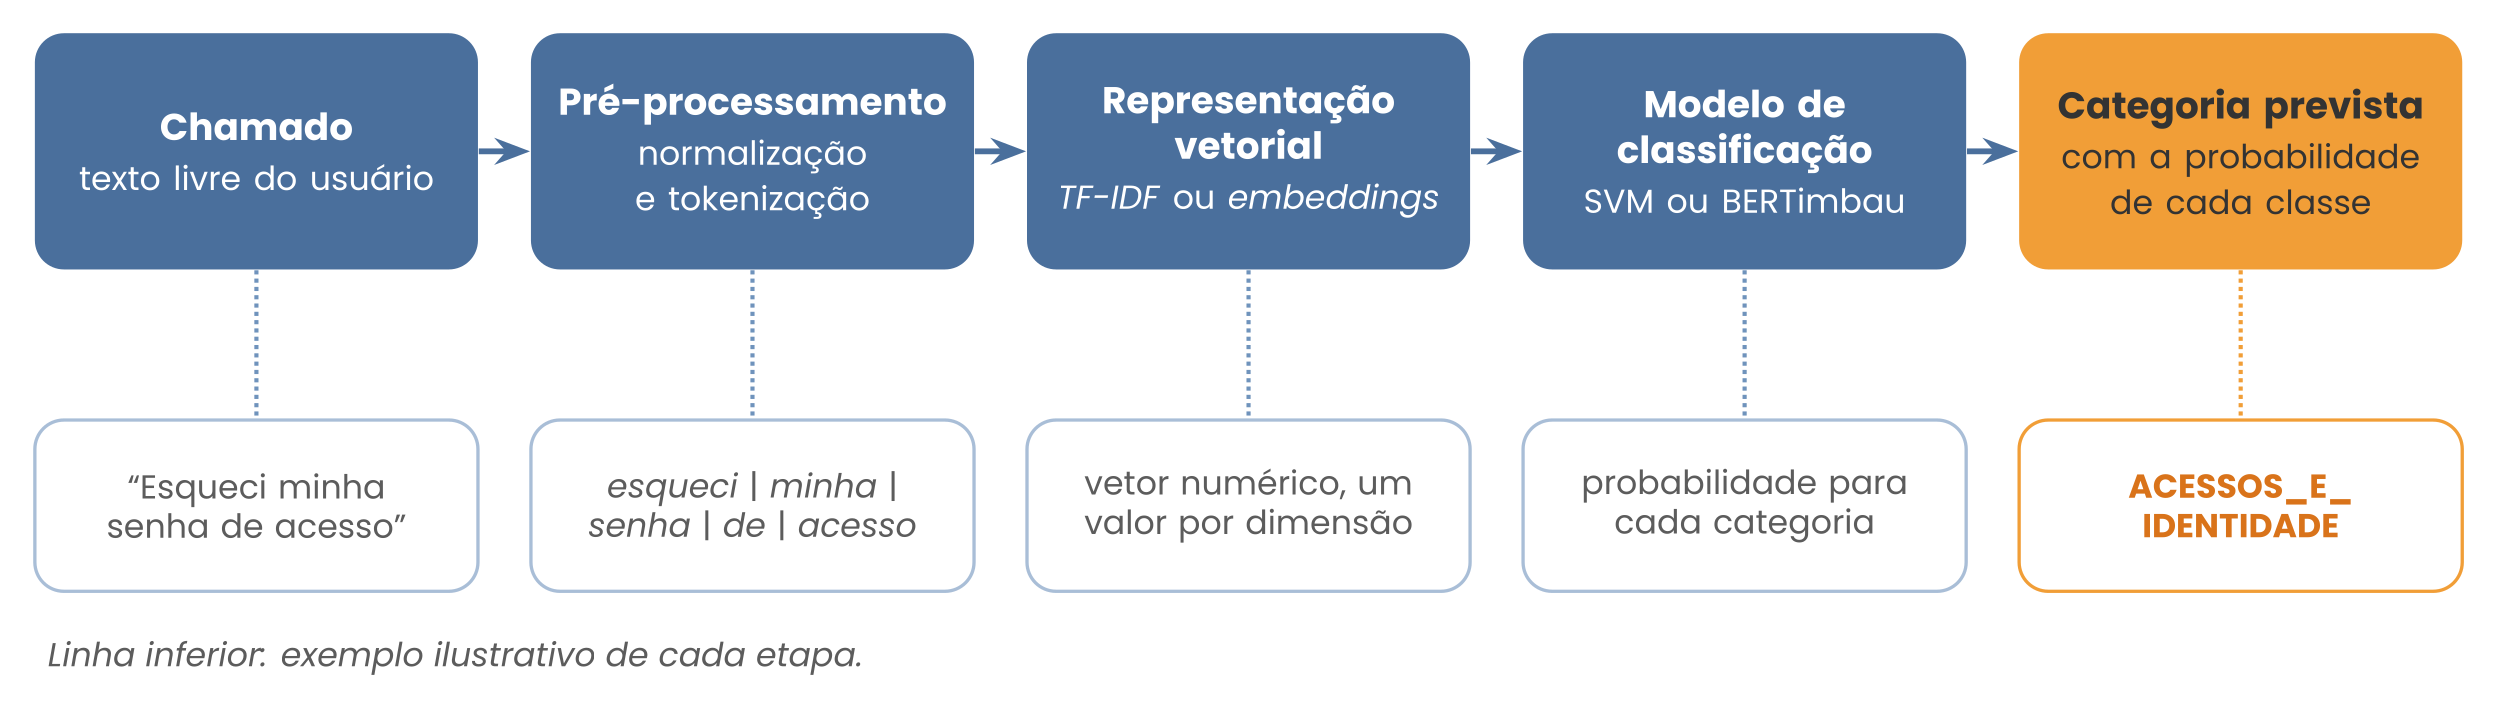
\includegraphics[width=\textwidth]{imagens/fluxo_pln.png}
    \legend{Fonte: Elaborado pelos autores.}
\end{figure}

\subsubsection{Representações vetoriais de texto}
\label{subsec:pln_representacoes}

% - - - - - - - - - - - - - - - - - - - - - - - - - - - - - - -
\subsubsubsection{\textit{TF-IDF} e modelos baseados em frequência}
\label{subsubsec:pln_tfidf}

A representação mais simples de um documento para fins de classificação é o modelo \textit{bag-of-words}: cada documento é representado como um vetor de contagens de palavras, sem considerar a ordem em que aparecem. O \textit{TF-IDF} é um refinamento desse modelo que pondera cada termo pelo produto de duas quantidades: a frequência do termo no documento (TF, de \textit{term frequency}) e o inverso de sua frequência no corpus (IDF, de \textit{inverse document frequency}), sendo o corpus o conjunto de textos usado como base, aqui os chamados. Com isso, reduz o peso de termos muito comuns e aumenta o peso de termos mais informativos.

Formalmente, o peso de um termo $t$ em um documento $d$ é
\begin{equation}
\mathrm{TF\text{-}IDF}(t,d) = \mathrm{tf}(t,d) \cdot \log \frac{N}{\mathrm{df}(t)}
\label{eq:tfidf}
\end{equation}
em que $\mathrm{tf}(t,d)$ é o número de vezes que o termo $t$ aparece no documento $d$, $N$ é o total de documentos do corpus e $\mathrm{df}(t)$ é o número de documentos que contêm $t$. Por exemplo, em um corpus hipotético de 1.000 chamados, um termo que aparece em 10 deles (como ``VPN'', de \textit{Virtual Private Network} -- Rede Privada Virtual) tem $\log_{10}(1000/10) = 2$, enquanto um que aparece em 500 (como ``acesso'') tem $\log_{10}(1000/500) \approx 0{,}3$: o termo raro pesa mais. O logaritmo deste exemplo está em base 10. Na implementação, o scikit-learn usa o logaritmo natural, com a suavização da Equação~\ref{eq:tfidf-sklearn}. % CONFERIDO: o exemplo e log10; o TfidfVectorizer usa ln.

Apesar de sua simplicidade, o \textit{TF-IDF} ainda é amplamente utilizado como \textit{baseline} em tarefas de classificação de texto, especialmente quando combinado com o SVM, um algoritmo que classifica textos encontrando a melhor separação possível entre as categorias, e apresenta desempenho competitivo em domínios com vocabulário técnico específico e baixa polissemia, ou seja, onde as palavras raramente mudam de sentido dependendo do contexto \cite{wahba2023}. Sua principal limitação é a incapacidade de capturar relações semânticas entre termos: palavras sinônimas ou semanticamente relacionadas são tratadas como completamente distintas.

% - - - - - - - - - - - - - - - - - - - - - - - - - - - - - - -
\subsubsubsection{\textit{Embeddings} estáticos: \textit{Word2Vec} e \textit{GloVe}}
\label{subsubsec:pln_embeddings}

Os \textit{embeddings} de palavras representam um avanço significativo em relação às abordagens baseadas em frequência, ao mapear cada palavra para um vetor denso em um espaço de baixa dimensionalidade, de forma que palavras semanticamente relacionadas sejam representadas por vetores próximos. O \textit{Word2Vec}, proposto por \citeonline{mikolov2013}, aprende \textit{embeddings} a partir de grandes corpora (plural de \textit{corpus}) textuais utilizando redes neurais rasas, treinadas para predizer palavras a partir de seu contexto ou contexto a partir de palavras.

O GloVe (\textit{Global Vectors for Word Representation} -- Vetores Globais para Representação de Palavras), proposto por \citeonline{pennington2014}, utiliza estatísticas globais de co-ocorrência do corpus para produzir representações com propriedades algébricas notáveis: vetores de palavras semanticamente relacionadas tendem a ser próximos no espaço vetorial, e operações aritméticas entre vetores refletem relações semânticas; o exemplo clássico é que o vetor de ``rei'' menos ``homem'' mais ``mulher'' resulta em um vetor próximo ao de ``rainha'' \cite{mikolov2013}.

Para tornar a ideia concreta, a Tabela~\ref{tab:embedding_exemplo} mostra um exemplo ilustrativo com vetores de quatro dimensões para três palavras do vocabulário de TI. Em um modelo real, os vetores têm centenas de dimensões e seus valores são aprendidos a partir do corpus. A proximidade entre dois vetores $u$ e $v$ costuma ser medida pela similaridade do cosseno \cite{mikolov2013,pennington2014}, que compara a direção deles:
\begin{equation}
\cos(u,v) = \frac{u \cdot v}{\lVert u \rVert \, \lVert v \rVert}
          = \frac{\sum_{j=1}^{n} u_j v_j}{\sqrt{\sum_{j=1}^{n} u_j^2}\,\sqrt{\sum_{j=1}^{n} v_j^2}}
\label{eq:cosseno}
\end{equation}
O valor vai de $-1$ (direções opostas) a $1$ (mesma direção); com vetores de valores não negativos, como os de contagem de palavras, fica entre 0 (sem relação) e 1 (vetores idênticos). Na representação \textit{bag-of-words}, ``senha'' e ``login'' seriam palavras sem relação alguma (similaridade do cosseno igual a 0). Nos \textit{embeddings}, a similaridade do cosseno entre os vetores de ``senha'' e ``login'' é alta, $\cos(\text{senha},\text{login}) = 1{,}00 / (1{,}068 \times 0{,}949) \approx 0{,}99$, enquanto a de ``senha'' e ``impressora'' é baixa (0,12).

\begin{table}[H]
    \centering
    \caption{Exemplo ilustrativo de \textit{embeddings} de quatro dimensões}
    \label{tab:embedding_exemplo}
    \begin{tabular}{lcccc}
        \toprule
        \textbf{Palavra} & \textbf{$d_1$} & \textbf{$d_2$} & \textbf{$d_3$} & \textbf{$d_4$} \\
        \midrule
        senha      & 0,8 & 0,1 & 0,7 & 0,0 \\
        login      & 0,7 & 0,2 & 0,6 & 0,1 \\
        impressora & 0,0 & 0,9 & 0,1 & 0,8 \\
        \bottomrule
    \end{tabular}

    \vspace{0.3cm}

    \begin{tabular}{lc}
        \toprule
        \textbf{Par de palavras} & \textbf{Similaridade do cosseno} \\
        \midrule
        senha -- login      & 0,99 \\
        senha -- impressora & 0,12 \\
        login -- impressora & 0,28 \\
        \bottomrule
    \end{tabular}
    \legend{Fonte: Elaborado pelos autores.\\ Nota: Valores ilustrativos, não aprendidos de um corpus.}
\end{table}

Esses \textit{embeddings} estáticos representaram um avanço expressivo na qualidade das representações textuais e foram amplamente adotados como camada de entrada em modelos de aprendizado profundo para PLN. No entanto, eles atribuem um único vetor a cada palavra, independentemente do contexto em que ela aparece, limitação conhecida como o problema da representação estática.

% - - - - - - - - - - - - - - - - - - - - - - - - - - - - - - -
\subsubsubsection{Limitações das representações estáticas: polissemia e contexto}
\label{subsubsec:pln_limitacoes}

O grande problema dos \textit{embeddings} estáticos é que eles não conseguem identificar quando uma palavra muda de sentido dependendo do contexto, como ``banco'', que pode ser um assento ou uma instituição financeira. Em textos técnicos de suporte de TI, isso se manifesta em termos como ``acesso'', ``serviço'' ou ``sistema'', que podem ter significados muito distintos dependendo do chamado.

Essa limitação motivou o desenvolvimento de representações contextualizadas, nas quais o \textit{embedding} de cada palavra é computado dinamicamente a partir do contexto completo da frase. Os modelos baseados na arquitetura \textit{Transformer} \cite{vaswani2017}, uma rede neural que relaciona cada palavra a todas as outras do texto, em particular o BERT \cite{devlin2019}, modelo dessa família treinado sobre grandes volumes de texto, representam a abordagem dominante nessa direção.

\subsubsection{Métricas de avaliação de classificadores}
\label{subsec:metricas_classificacao}

Para comparar classificadores, calculam-se métricas sobre os chamados do conjunto de teste, separado do treino e da validação. As mais usadas em classificação de texto são as abaixo.

\begin{itemize}
\item \textbf{Acurácia (\textit{accuracy})}: proporção de classificações corretas sobre o total de instâncias avaliadas.
\item \textbf{Precisão (\textit{precision})}: proporção de classificações corretas entre os casos previstos para uma determinada categoria, medindo a capacidade do modelo de evitar falsos positivos.
\item \textbf{Revocação (\textit{recall})}: capacidade do modelo de identificar corretamente os chamados pertencentes a cada categoria, medindo a capacidade de evitar falsos negativos.
\item \textbf{F1-score}: média harmônica entre precisão e revocação. Utiliza-se a variante \textbf{F1-macro}, que calcula o \textit{F1-score} de cada categoria e tira a média, tratando todas as categorias com o mesmo peso, independentemente do tamanho. Isso é especialmente importante em conjuntos de dados desbalanceados, nos quais algumas categorias têm muito mais chamados do que outras.
\item \textbf{Matriz de confusão}: representação tabular que detalha os tipos de erros cometidos pelo modelo, permitindo identificar padrões sistemáticos de confusão entre categorias semanticamente próximas.
\end{itemize}

Sejam $VP_c$, $FP_c$ e $FN_c$ os verdadeiros positivos, falsos positivos e falsos negativos da categoria $c$; $N$ o número de chamados avaliados; $K$ o número de categorias; $y_i$ a categoria real e $\hat y_i$ a prevista para o chamado $i$. As métricas são calculadas por
\begin{equation}
\mathrm{Acurácia} = \frac{1}{N} \sum_{i=1}^{N} \mathbf{1}\left[\hat{y}_i = y_i\right]
\label{eq:acuracia}
\end{equation}
\begin{equation}
P_c = \frac{VP_c}{VP_c + FP_c}
\label{eq:precisao}
\end{equation}
\begin{equation}
R_c = \frac{VP_c}{VP_c + FN_c}
\label{eq:revocacao}
\end{equation}
\begin{equation}
F1_c = \frac{2\, P_c\, R_c}{P_c + R_c}
\label{eq:f1}
\end{equation}
\begin{equation}
F1_{\mathrm{macro}} = \frac{1}{K} \sum_{c=1}^{K} F1_c, \qquad
P_{\mathrm{macro}} = \frac{1}{K} \sum_{c=1}^{K} P_c, \qquad
R_{\mathrm{macro}} = \frac{1}{K} \sum_{c=1}^{K} R_c
\label{eq:macro}
\end{equation}
Uma categoria sem nenhum acerto tem $F1_c = 0$ e reduz o F1-macro na mesma proporção que qualquer outra categoria.

\subsubsection{Abordagens de aprendizado de máquina para classificação automática de chamados}
\label{subsec:helpdesk_ml}

A automação da triagem de chamados por meio de aprendizado de máquina tem sido investigada na literatura \cite{zemp2021,wahba2023,yokota2025,razma2026}. O problema é tratado como uma tarefa de classificação supervisionada de texto: dado o histórico de chamados já categorizados, treina-se um modelo capaz de predizer a categoria de novos chamados a partir de sua descrição textual.

% - - - - - - - - - - - - - - - - - - - - - - - - - - - - - - -
\subsubsubsection{Modelos clássicos: \textit{Naive Bayes} e SVM com TF-IDF}
\label{subsubsec:helpdesk_classicos}

As primeiras abordagens automatizadas para classificação de chamados utilizaram algoritmos clássicos de aprendizado de máquina combinados com representações baseadas em frequência de termos. \citeonline{harun2023} investigaram a classificação automática de perguntas em um sistema de \textit{help desk} universitário, comparando \textit{Naive Bayes} e SVM, com vetorização TF-IDF, representação que pondera cada palavra pela frequência no chamado e pela raridade no conjunto de chamados (Seção~\ref{subsubsec:pln_tfidf}). O \textit{Naive Bayes}, ou Bayes ingênuo, é um classificador probabilístico que supõe que as palavras são independentes entre si. O SVM (\textit{Support Vector Machine} -- Máquina de Vetores de Suporte) é um classificador linear e não probabilístico, ou seja, separa as categorias por uma fronteira em vez de calcular probabilidades. Os resultados demonstraram que o SVM com TF-IDF supera o \textit{Naive Bayes} em acurácia (métrica definida na Seção~\ref{subsec:metricas_classificacao}), estabelecendo-se como referência para abordagens clássicas nesse domínio.

Apesar de sua eficiência computacional e facilidade de interpretação, esses modelos apresentam limitações na captura de relações semânticas entre termos. A representação TF-IDF trata cada palavra de forma independente, sem considerar o contexto em que ela aparece, o que restringe a capacidade do modelo de distinguir categorias semanticamente próximas.

% - - - - - - - - - - - - - - - - - - - - - - - - - - - - - - -
\subsubsubsection{Redes neurais convolucionais aplicadas a chamados}
\label{subsubsec:helpdesk_cnn}

Com o avanço das técnicas de aprendizado profundo, modelos baseados em CNN passaram a ser aplicados à classificação de chamados de suporte. \citeonline{paramesh2022} propuseram um classificador baseado em CNN com \textit{word embeddings} (representações vetoriais densas de palavras aprendidas por redes neurais) para categorização automática de chamados de \textit{service desk} de infraestrutura de TI. Os autores compararam o modelo proposto com SVM, \textit{Naive Bayes}, Regressão Logística e \textit{K-Nearest Neighbor}, e a CNN obteve a maior acurácia (91,20\%) e o maior \textit{F1-score} (91,02\%) no conjunto de teste, contra 87,43\% e 87,36\% do SVM, o melhor dos modelos clássicos.

A vantagem das CNN em relação aos modelos clássicos reside na capacidade de identificar automaticamente quais grupos de palavras que aparecem juntas são importantes para a classificação, sem que um especialista precise definir isso manualmente. Essa progressão de modelos lineares com TF-IDF para redes profundas com \textit{embeddings} estabelece o contexto histórico sobre o qual os modelos baseados em \textit{transformers} representam um novo salto qualitativo.

% - - - - - - - - - - - - - - - - - - - - - - - - - - - - - - -
\subsubsubsection{Classificação de chamados no contexto brasileiro}
\label{subsubsec:helpdesk_brasil}

A literatura sobre classificação automática de chamados de suporte em português brasileiro ainda é escassa, e os trabalhos existentes evidenciam limitações importantes das abordagens mais simples nesse contexto específico.

\citeonline{pereira2023} apresentaram um modelo de classificação automática de chamados de suporte de TI em sete categorias, baseado em uma rede neural totalmente conectada cuja entrada são as 500 palavras mais frequentes do conjunto de treino. O modelo foi treinado e testado com 2.229 chamados de uma empresa de suporte de TI da região de Florianópolis, em vários idiomas (principalmente inglês, alemão, português e espanhol), e atingiu 75\% de precisão média, com revocação média e acurácia também de 75\%. Os autores disponibilizaram publicamente o código, o modelo e os dados anonimizados, e desenvolveram um protótipo \textit{web} com \textit{backend} e \textit{frontend} para uso dos analistas de TI, tornando-o um dos poucos trabalhos nacionais com \textit{dataset} público e interface funcional. No entanto, a acurácia de 75\% deixa margem considerável para melhoria, especialmente em cenários com maior número de categorias ou com classes semanticamente próximas.

\citeonline{yokota2025} investigou a classificação hierárquica de chamados de suporte ao cliente em português brasileiro (PT-BR) utilizando \textit{Naive Bayes} e MLP (\textit{Multilayer Perceptron} -- Perceptron Multicamadas) com duas variações arquiteturais, sobre \textit{embeddings} do modelo Multilingual E5 (\textit{EmbEddings from bidirEctional Encoder rEpresentations} -- \textit{Embeddings} a partir de Representações de Codificador Bidirecional). Os resultados, avaliados por F1-macro para lidar com o desbalanceamento entre classes, foram limitados (no máximo 61\%), o que a autora associa ao desbalanceamento, à proximidade semântica entre categorias e ao vocabulário especializado. A autora conclui que a abordagem proposta revelou desafios substanciais na classificação automática de textos especializados, evidenciando a necessidade de abordagens metodológicas mais sofisticadas, o que motiva avaliar o ajuste fino do BERTimbau neste trabalho.

% ---------------------------------------------------------------
\subsection{O modelo BERT e suas variantes}

Modelos de linguagem baseados na arquitetura \textit{Transformer} \cite{vaswani2017} aprendem representações contextualizadas de texto por meio de mecanismos de atenção que consideram simultaneamente todas as posições de uma sequência de entrada. O BERT \cite{devlin2019} é um modelo desta família, pré-treinado sobre texto sem rótulos e adaptado a tarefas como a classificação de texto por \textit{fine-tuning}. O BERTimbau \cite{souza2020} é uma variante do BERT pré-treinada especificamente sobre corpora em português brasileiro.

\subsubsection{Arquitetura \textit{Transformer} e mecanismo de atenção}
\label{subsec:bert_transformer}

% - - - - - - - - - - - - - - - - - - - - - - - - - - - - - - -
\subsubsubsection{\textit{Self-attention} e atenção bidirecional}
\label{subsubsec:bert_attention}

A arquitetura \textit{Transformer} é composta por dois blocos principais: 
um \textit{encoder} (codificador) e um \textit{decoder} (decodificador), 
cada um formado por camadas empilhadas \cite{vaswani2017}. O \textit{encoder} 
é responsável por receber a sequência de entrada e transformá-la em 
representações vetoriais ricas em informação contextual. O \textit{decoder}, 
por sua vez, utiliza essas representações para gerar a sequência de saída como uma tradução ou resposta. Cada camada do \textit{encoder} é composta 
por dois subcomponentes principais: o mecanismo de \textit{self-attention}, 
que permite que cada \textit{token}, ou seja, cada unidade mínima de texto em que 
o modelo divide a entrada, ``observe'' todos os outros da sequência, 
e uma rede neural densa aplicada posição a posição (\textit{feed-forward 
network}). O resultado de cada subcomponente passa por uma conexão residual seguida de normalização (\textit{layer normalization}) \cite{vaswani2017}.

Vale destacar que modelos como o BERT utilizam apenas 
o bloco \textit{encoder}, pois seu objetivo é produzir representações 
contextuais do texto de entrada, e não gerar novas sequências \cite{devlin2019}.

A Figura~\ref{fig:transformer} resume essa estrutura. O BERT utiliza apenas o bloco da esquerda, o \textit{encoder}.
 
\begin{figure}[H]
    \caption{Arquitetura \textit{Transformer} simplificada}
    \label{fig:transformer}
    \centering
    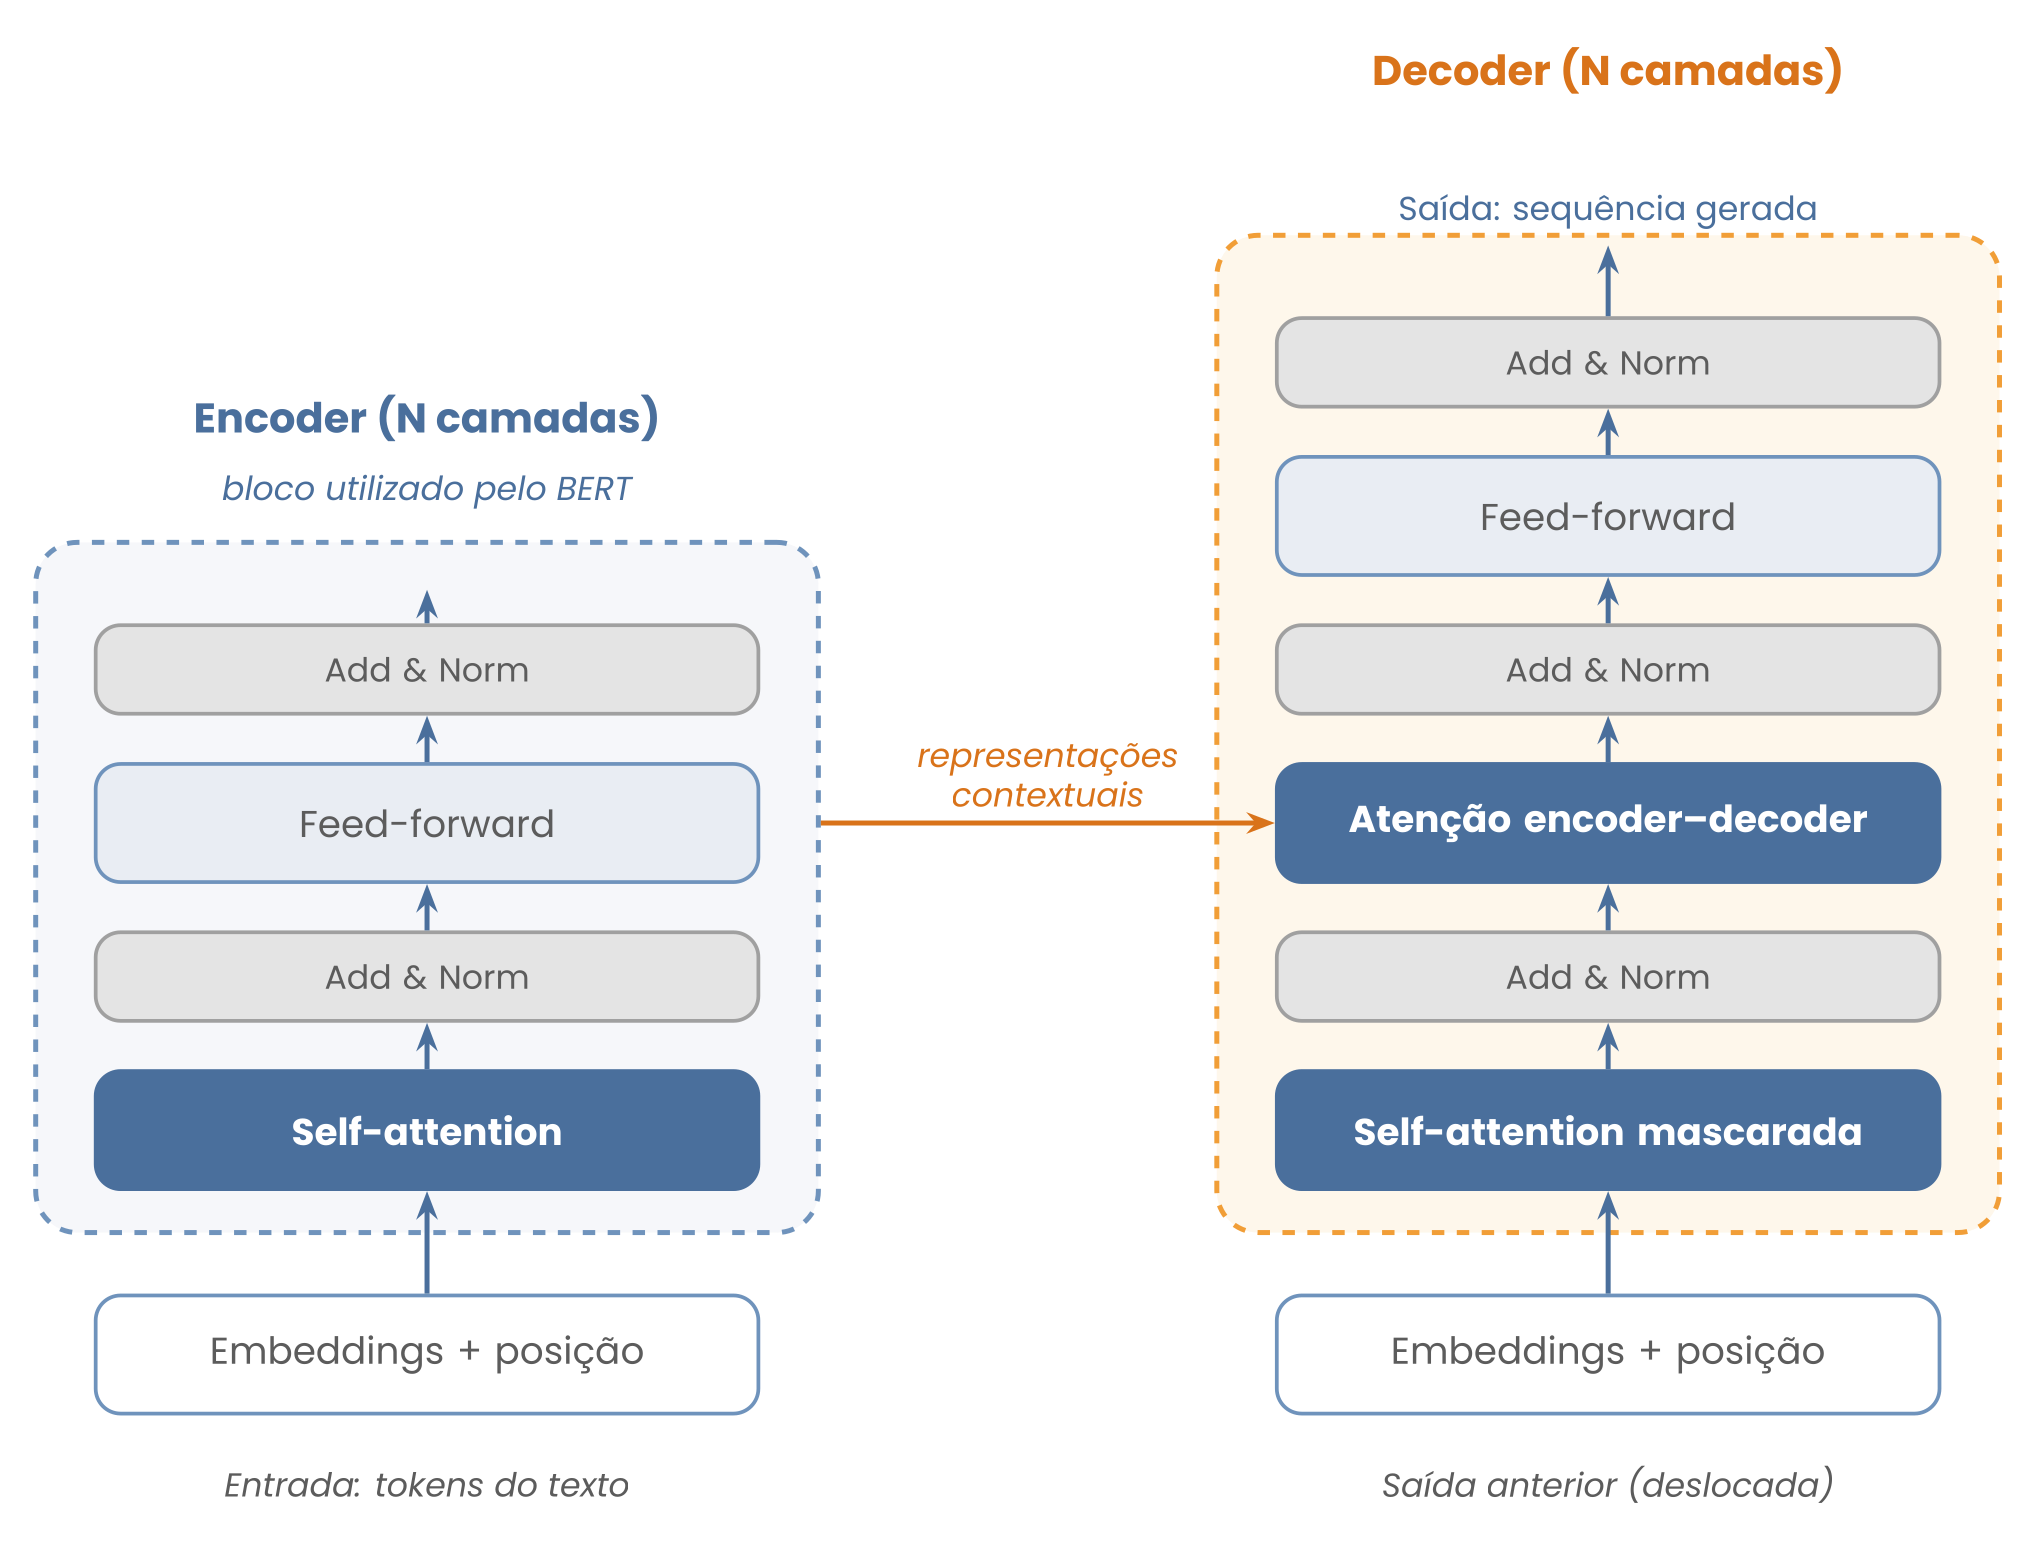
\includegraphics[width=0.85\textwidth]{imagens/transformer_arquitetura.png}
    \legend{Fonte: Elaborado pelos autores, com base em \citeonline{vaswani2017}.}
\end{figure}

A arquitetura \textit{Transformer}, proposta por \citeonline{vaswani2017}, apresentou o primeiro modelo de transdução baseado inteiramente em \textit{self-attention}, sem recorrência nem convolução alinhada à sequência, como alternativa às redes recorrentes. As RNN (\textit{Recurrent Neural Network} -- Rede Neural Recorrente) são uma classe de redes neurais 
projetadas para processar dados sequenciais, nos quais o contexto e a ordem 
temporal importam, processando os \textit{tokens} um por vez, da esquerda para 
a direita. As LSTM (\textit{Long Short-Term Memory} -- Memória de Longo e Curto Prazo) são um tipo especializado 
de RNN projetado para aprender dependências de longo prazo em sequências, 
mitigando o problema de desvanecimento do gradiente presente nas RNN simples. 
Apesar dessas melhorias, ambas as arquiteturas ainda processam a sequência de 
forma estritamente sequencial, o que limita o paralelismo computacional e 
dificulta a captura de relações entre termos distantes.

Para compreender o mecanismo de atenção, considere a frase ``o banco bloqueou 
meu acesso'': para determinar o significado da palavra ``banco'', é necessário 
considerar as demais palavras da frase, especialmente ``bloqueou'' e ``acesso'', que indicam tratar-se de uma instituição financeira e não de um assento. O 
\textit{self-attention} formaliza esse processo: para cada \textit{token} da 
sequência, o mecanismo calcula um \textit{score} de relevância em relação a todos os 
outros \textit{tokens}, indicando o quanto cada um deve ``influenciar'' a 
representação do \textit{token} atual. ``Atender simultaneamente a todas as 
posições'' significa que esse cálculo é realizado em paralelo para todos os 
pares de \textit{tokens} da sequência, possibilitando a captura de dependências 
de longo alcance de forma muito mais eficiente do que as arquiteturas recorrentes.

A Figura~\ref{fig:self_attention} ilustra esse cálculo para a palavra ``banco'': os pesos de atenção, que somam 1, indicam o quanto cada \textit{token} contribui para a nova representação de ``banco''. Nesse exemplo, ``acesso'' e ``bloqueou'' recebem os maiores pesos, o que leva o modelo a representar ``banco'' como instituição financeira.
 
\begin{figure}[H]
    \caption{Exemplo ilustrativo de \textit{self-attention} para o \textit{token} ``banco''}
    \label{fig:self_attention}
    \centering
    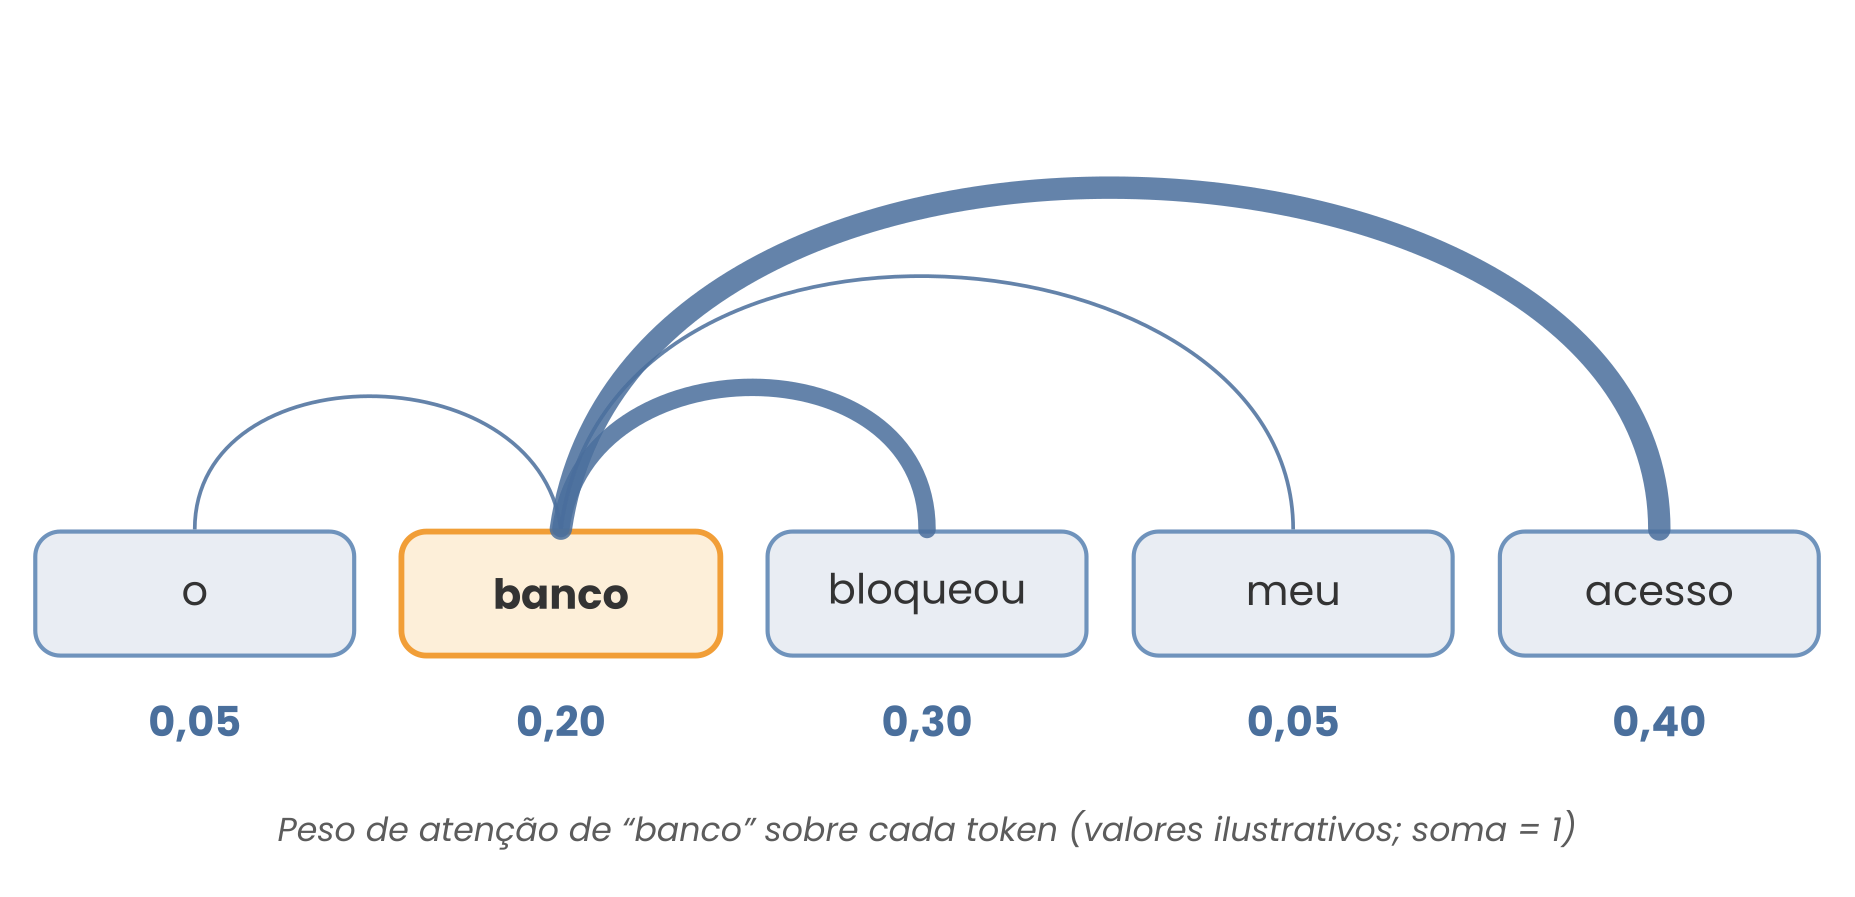
\includegraphics[width=0.85\textwidth]{imagens/self_attention.png}
    \legend{Fonte: Elaborado pelos autores.\\ Nota: Valores ilustrativos, não extraídos de um modelo treinado.}
\end{figure}

Para as matrizes de consultas $Q$, chaves $K$ e valores $V$, obtidas por projeções lineares das representações de entrada, a atenção é calculada como em \citeonline{vaswani2017}:
\begin{equation}
\mathrm{Atenção}(Q,K,V) = \mathrm{softmax}\!\left( \frac{Q K^{\top}}{\sqrt{d_k}} \right) V
\label{eq:atencao}
\end{equation}
em que $d_k$ é a dimensão das chaves. A divisão por $\sqrt{d_k}$ evita valores muito grandes antes da \textit{softmax}. Cada linha da matriz $\mathrm{softmax}(\cdot)$ soma 1 e contém os pesos de atenção de um \textit{token} em relação a todos os outros, como na Figura~\ref{fig:self_attention}. O \textit{BERT-base} usa 12 atenções em paralelo (\textit{multi-head}) em cada uma de suas 12 camadas.

Modelos como o GPT (\textit{Generative Pre-trained Transformer} -- Transformer Generativo Pré-treinado) utilizam atenção unidirecional (cada \textit{token} só pode 
atender aos \textit{tokens} anteriores). O BERT, por sua vez, utiliza atenção 
bidirecional: cada \textit{token} atende simultaneamente a todos os outros 
\textit{tokens} da sequência, tanto os que aparecem antes quanto os que aparecem 
depois. Essa bidirecionalidade é fundamental para a qualidade das representações 
contextualizadas geradas pelo modelo, uma vez que o significado de uma palavra 
frequentemente depende tanto de seu contexto anterior quanto posterior 
\cite{devlin2019}.

A Figura~\ref{fig:atencao_bidirecional} compara os dois tipos de atenção: na atenção unidirecional, cada \textit{token} só atende a si mesmo e aos anteriores; na bidirecional, atende a todos.
 
\begin{figure}[H]
    \caption{Atenção unidirecional e atenção bidirecional}
    \label{fig:atencao_bidirecional}
    \centering
    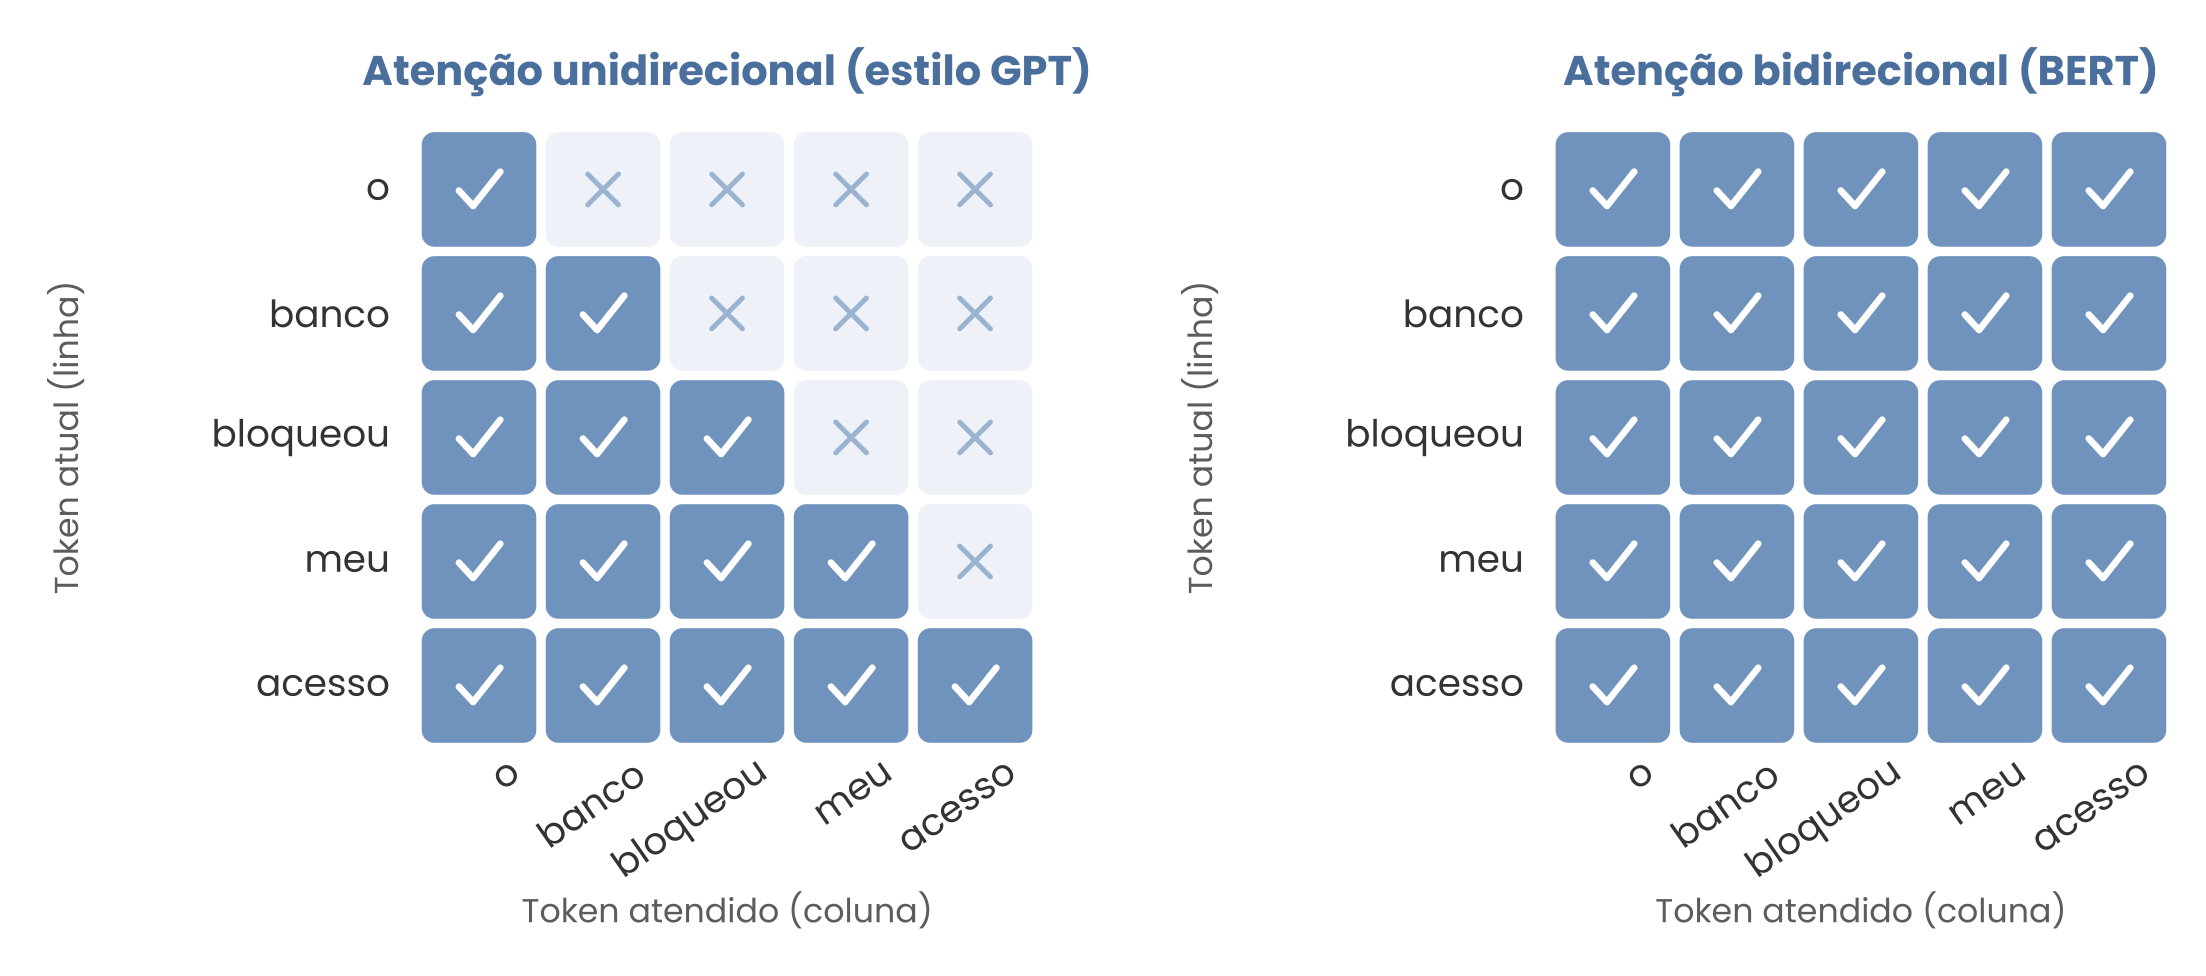
\includegraphics[width=0.9\textwidth]{imagens/atencao_bidirecional.png}
    \legend{Fonte: Elaborado pelos autores.\\ Nota: Cada linha indica a quais \textit{tokens} a palavra daquela linha pode atender.}
\end{figure}

% - - - - - - - - - - - - - - - - - - - - - - - - - - - - - - -
\subsubsubsection{Pré-treinamento: \textit{Masked Language Modeling} e \textit{Next Sentence Prediction}}
\label{subsubsec:bert_pretrain}

O BERT é pré-treinado em dois objetivos complementares sobre grandes corpora textuais não rotulados. O primeiro, MLM (\textit{Masked Language Modeling} -- Modelagem de Linguagem com Máscara), mascara aleatoriamente 15\% dos \textit{tokens} de cada sequência de entrada e treina o modelo para predizer os \textit{tokens} mascarados a partir do contexto bidirecional restante. Esse objetivo força o modelo a aprender representações ricas que capturam o significado de cada palavra em seu contexto completo \cite{devlin2019}.

O segundo objetivo, NSP (\textit{Next Sentence Prediction} -- Predição da Próxima Sentença), treina o modelo a determinar se duas sentenças apresentadas em sequência são consecutivas no texto original ou foram pareadas aleatoriamente. Esse objetivo permite ao modelo aprender relações semânticas entre sentenças, o que é útil para tarefas como inferência textual e resposta a perguntas.

% - - - - - - - - - - - - - - - - - - - - - - - - - - - - - - -
\subsubsubsection{\textit{Fine-tuning} para tarefas \textit{downstream}}
\label{subsubsec:bert_finetune}

Após o pré-treinamento, o BERT pode ser adaptado para tarefas específicas por meio do processo de \textit{fine-tuning}: o modelo pré-treinado é inicializado com os pesos aprendidos no pré-treinamento, uma camada de saída específica para a tarefa é adicionada ao topo da arquitetura, e o modelo completo é treinado por um número reduzido de épocas sobre o conjunto de dados rotulado da tarefa-alvo \cite{devlin2019}.

Essa abordagem de pré-treinamento seguido de \textit{fine-tuning} é particularmente eficaz porque o modelo já adquiriu conhecimento linguístico geral durante o pré-treinamento, e o \textit{fine-tuning} apenas adapta esse conhecimento para o domínio e a tarefa específicos. Para classificação de chamados de TI, o \textit{fine-tuning} ajusta os pesos do modelo para que as representações produzidas sejam especialmente discriminativas entre as categorias de chamados presentes no \textit{dataset}.

\subsubsection{BERT}
\label{subsec:bert_modelo}

% - - - - - - - - - - - - - - - - - - - - - - - - - - - - - - -
\subsubsubsection{Arquitetura e configurações \textit{BERT-base} e \textit{BERT-large}}
\label{subsubsec:bert_arquitetura}

\citeonline{devlin2019} propuseram o BERT em duas configurações. O \textit{BERT-base} possui 12 camadas de \textit{encoder} \textit{Transformer}, dimensão oculta de 768, 12 cabeças de atenção e 110 milhões de parâmetros; o \textit{BERT-large} possui 24 camadas, dimensão de 1.024, 16 cabeças de atenção e 340 milhões de parâmetros. Ambas as versões foram pré-treinadas sobre o corpus da Wikipedia em inglês e o BookCorpus, totalizando aproximadamente 3,3 bilhões de palavras.

O BERT estabeleceu o estado da arte em onze tarefas de PLN no momento 
de sua publicação, incluindo classificação de sentenças, resposta a perguntas e inferência textual \cite{devlin2019}. Seu lançamento popularizou o uso de modelos pré-treinados em tarefas 
de PLN, consolidando a abordagem de pré-treinamento em larga escala 
seguido de \textit{fine-tuning} como a estratégia dominante para 
tarefas de PLN.

% - - - - - - - - - - - - - - - - - - - - - - - - - - - - - - -
\subsubsubsection{\textit{Token} [CLS] e classificação de sequências}
\label{subsubsec:bert_cls}

Para tarefas de classificação de sequências, o BERT utiliza um \textit{token} especial [CLS] (abreviação de \textit{Classification}, marcador inserido pelo modelo para agregar a representação global da sequência) inserido no início de cada sequência de entrada. Após o processamento pelas camadas de \textit{encoder}, a representação vetorial correspondente ao [CLS] agrega informação contextual de toda a sequência e é usada como entrada para a camada de classificação \cite{devlin2019}. Durante o \textit{fine-tuning}, essa camada de classificação, tipicamente uma camada \textit{linear} seguida de \textit{softmax}, aprende a mapear a representação do [CLS] para as probabilidades de cada categoria. A camada linear produz uma pontuação $z_k$ para cada categoria $k$, e a \textit{softmax} converte essas pontuações em probabilidades, $p_k = e^{z_k} / \sum_{j} e^{z_j}$, todas positivas e com soma igual a 1. Por exemplo, as pontuações 2, 1 e 0 viram probabilidades de cerca de 0,67, 0,24 e 0,09, e a categoria prevista é a de maior probabilidade.

Sobre a representação final do \textit{token} [CLS], $h_{[CLS]} \in \mathbb{R}^{768}$, a probabilidade de cada categoria $c$ é
\begin{equation}
p(c \mid x) = \mathrm{softmax}\!\left( W\, h_{[CLS]} + b \right)_c, \qquad
W \in \mathbb{R}^{K \times 768},\; b \in \mathbb{R}^{K}
\label{eq:cabeca}
\end{equation}
O modelo inteiro é ajustado minimizando a entropia cruzada sobre os $N$ chamados de treino:
\begin{equation}
\mathcal{L} = -\frac{1}{N} \sum_{i=1}^{N} \log p(y_i \mid x_i)
\label{eq:entropia}
\end{equation}
A categoria prevista é $\hat y = \arg\max_c p(c \mid x)$, e a confiança exibida na interface é $\max_c p(c \mid x)$.

\subsubsection{BERTimbau: BERT para o português brasileiro}
\label{subsec:bertimbau}

% - - - - - - - - - - - - - - - - - - - - - - - - - - - - - - -
\subsubsubsection{Corpus de pré-treinamento e diferenças em relação ao mBERT}
\label{subsubsec:bertimbau_corpus}

\citeonline{souza2020} desenvolveram o BERTimbau a partir do BrWaC (\textit{Brazilian Web as Corpus}), um grande corpus de páginas \textit{web} em português com 2,68 bilhões de \textit{tokens}. Duas versões foram disponibilizadas: BERTimbau-base (12 camadas, 110M parâmetros) e BERTimbau-large (24 camadas, 335M parâmetros; o artigo arredonda esse total para 330M).

A principal diferença em relação ao mBERT (\textit{Multilingual BERT} -- BERT Multilíngue) está no foco linguístico: o mBERT foi pré-treinado sobre 104 idiomas simultaneamente \cite{pires2019}, o que tende a diluir a capacidade de representação para cada língua individualmente. O BERTimbau, ao ser pré-treinado exclusivamente sobre texto em português brasileiro, aprende padrões morfológicos, sintáticos e semânticos específicos do idioma com maior profundidade.

% - - - - - - - - - - - - - - - - - - - - - - - - - - - - - - -
\subsubsubsection{Desempenho em tarefas de PLN em PT-BR}
\label{subsubsec:bertimbau_desempenho}

\citeonline{souza2020} avaliaram o BERTimbau em três tarefas de PLN em português: reconhecimento de entidades nomeadas (NER, do inglês \textit{Named Entity Recognition}), similaridade textual entre sentenças e inferência textual (\textit{Recognizing Textual Entailment}). O modelo obteve desempenho de estado da arte nas três tarefas, como mostra a Tabela~\ref{tab:bertimbau_sota}, consolidando-se como referência para aplicações de PLN em PT-BR. Na versão \textit{base}, o BERTimbau superou o mBERT e o melhor resultado anterior nas quatro medidas da tabela.

\begin{table}[htb]
  \centering
  \caption{Desempenho do BERTimbau-base em tarefas de PLN em português}
  \label{tab:bertimbau_sota}
  \footnotesize
  \setlength{\tabcolsep}{3pt}
  \begin{tabular}{p{5.2cm}p{3.3cm}ccc}
    \toprule
    Tarefa (conjunto de avaliação) & Métrica & BERTimbau-base & mBERT & Melhor anterior \\
    \midrule
    Similaridade textual (ASSIN2) & Correlação de Pearson & 0,836 & 0,809 & 0,83 \\
    Inferência textual (ASSIN2) & F1 (\%) & 89,2 & 86,8 & 88,3 \\
    NER no MiniHAREM (5 classes, com CRF) & F1 (\%) & 83,1 & 79,2 & 82,3 \\
    NER no MiniHAREM (10 classes, com CRF) & F1 (\%) & 77,6 & 73,1 & 74,6 \\
    \bottomrule
  \end{tabular}
  \legend{Fonte: Adaptado de \citeonline{souza2020}.\\ Nota: Nas linhas de NER, os valores do BERTimbau-base e do mBERT são das versões com camada CRF (\textit{Conditional Random Field}) sobre o BERT. A versão \textit{large} obteve valores ainda maiores (0,852; 90,0; 83,7 e 78,5).}
\end{table}

\subsubsection{\textit{Fine-tuning} de BERT para classificação de chamados de TI}
\label{subsec:bert_tickets}

A aplicação de BERT e modelos derivados à classificação de chamados de TI tem demonstrado resultados expressivos na literatura recente. \citeonline{borges2024} realizou uma comparação sistemática entre BERT e algoritmos clássicos, SVM e \textit{Naive Bayes}, em tarefas de classificação de texto em português e inglês, utilizando quatro \textit{datasets} públicos, nenhum deles de chamados de TI. 

O BERT obteve, em geral, acurácia e F1 superiores, com vantagem mais clara em bases maiores e mais equilibradas; em bases menores, a diferença foi menos expressiva (na Fake.br, o BERTimbau, o \textit{Naive Bayes} e o SVM ficaram na faixa dos 60\%). O autor destaca ainda o custo computacional significativamente maior do BERT.

\citeonline{zemp2021} comparou CNN, BiLSTM (\textit{Bidirectional Long Short-Term Memory} -- Memória de Longo e Curto Prazo Bidirecional) e RoBERTa (\textit{Robustly Optimized BERT Pretraining Approach} -- Abordagem de Pré-treinamento do BERT Robustamente Otimizada) em chamados reais de um banco (Seção~\ref{subsubsec:helpdesk_caixapreta}). A melhor CNN atingiu F1-macro de 0,75. Com o \textit{fine-tuning} simples, o DistilRoBERTa, versão reduzida do RoBERTa, ficou abaixo desse valor (0,72); somente após um pré-treinamento adicional do modelo de linguagem com os próprios chamados ele superou a CNN, por uma margem de 0,018.

\citeonline{razma2026} compararam regressão logística com TF-IDF 
frente a mBERT e XLM-RoBERTa (\textit{Cross-lingual Language Model RoBERTa} -- Modelo de Linguagem Multilíngue RoBERTa), uma variante do RoBERTa desenvolvida 
especificamente para lidar com múltiplos idiomas simultaneamente, 
em um corpus de 87 mil chamados multilíngues de uma empresa 
de manufatura. Os resultados confirmaram que \textit{transformers} 
superam modelos clássicos em macro-F1, especialmente para classes 
de baixa frequência e semanticamente complexas. Os autores aplicaram o LIME ao mBERT e à regressão logística, e o SHAP à regressão logística, o que mostra ser viável explicar um BERT \textit{fine-tuned} com LIME sobre chamados reais de ITSM; eles afirmam que a comparação mostra como os modelos \textit{transformer} capturam relações semânticas mais sutis, o que favorece a interpretabilidade e a confiança.

% ---------------------------------------------------------------
\subsection{Inteligência Artificial Explicável (XAI)}

Inteligência Artificial Explicável (XAI, do inglês \textit{Explainable Artificial Intelligence}) refere-se ao conjunto de métodos que tornam mais compreensíveis e transparentes os modelos de aprendizado de máquina do tipo caixa-preta \cite{salih2023}. O LIME \cite{ribeiro2016} e o SHAP \cite{lundberg2017} são dois métodos \textit{post-hoc} de XAI.

\subsubsection{Definição e motivação}
\label{subsec:xai_definicao}

% - - - - - - - - - - - - - - - - - - - - - - - - - - - - - - -
\subsubsubsection{O problema da caixa-preta em aprendizado profundo}
\label{subsubsec:xai_caixapreta}

Modelos de aprendizado profundo, incluindo o BERT, são frequentemente descritos como caixas-pretas: produzem predições com alta acurácia, mas sem revelar quais características da entrada determinaram a saída. Isso acontece porque esses modelos possuem mais de cem milhões de 
parâmetros internos, valores numéricos ajustados durante o 
treinamento, organizados em múltiplas camadas de cálculos complexos. Essa estrutura dificulta para um ser humano acompanhar ou explicar, passo a passo, como o modelo chegou a uma determinada decisão \cite{salih2023}.

Em contextos como a triagem de chamados de TI, essa opacidade representa um problema prático concreto. Analistas de suporte e gestores precisam auditar as decisões do sistema, identificar erros sistemáticos e eventualmente contestar categorizações incorretas. Um modelo que não fornece justificativa para suas predições é difícil de depurar, difícil de melhorar e difícil de justificar perante \textit{stakeholders} (partes interessadas, como gestores e diretores) organizacionais.

% - - - - - - - - - - - - - - - - - - - - - - - - - - - - - - -
\subsubsubsection{Confiança, explicabilidade e adoção em produção}
\label{subsubsec:xai_confianca}

No estudo de \citeonline{zemp2021}, a equipe de suporte recusou parte do sistema de classificação, como discutido na Seção~\ref{subsubsec:helpdesk_caixapreta}. 

\citeonline{razma2026} ilustram, com LIME (e também SHAP), que o BERT atribui pesos mais contextuais aos termos do que a regressão logística e afirmam que essa comparação mostra como modelos \textit{transformer} capturam relações semânticas mais sutis, o que favorece a interpretabilidade e a confiança em sistemas de automação, embora não tenham medido a reação dos operadores.

Essa ideia é consistente com a literatura de XAI mais ampla: as explicações
 ajudam os usuários a decidir se confiam em uma predição e a identificar modelos 
 que erram por razões inadequadas \cite{ribeiro2016}.


% - - - - - - - - - - - - - - - - - - - - - - - - - - - - - - -
\subsubsubsection{Taxonomia de métodos XAI: intrínsecos versus \textit{post-hoc}, locais versus globais}
\label{subsubsec:xai_taxonomia}

Os métodos de XAI costumam ser classificados segundo duas dimensões principais. A primeira dimensão distingue métodos intrínsecos dos métodos \textit{post-hoc}. Métodos intrínsecos são aqueles em que a interpretabilidade é uma propriedade do próprio modelo: árvores de decisão, regressão logística e modelos lineares em geral são interpretáveis por construção, pois seus parâmetros têm significado diretamente interpretável. Métodos \textit{post-hoc} são aplicados após o treinamento, sobre modelos de qualquer complexidade, e produzem explicações sem modificar o modelo original.

A segunda dimensão distingue explicações locais das globais. Explicações locais descrevem o comportamento do modelo para uma instância específica de entrada (exemplo: por que o modelo classificou \textit{este} chamado como ``Acesso''?). Explicações globais descrevem o comportamento geral do modelo (exemplo: quais termos são mais importantes para cada categoria em média?). SHAP e LIME são métodos \textit{post-hoc} que operam primariamente no nível local, embora o SHAP permita agregações que produzem explicações globais.

\subsubsection{LIME: \textit{Local Interpretable Model-Agnostic Explanations}}
\label{subsec:lime}

% - - - - - - - - - - - - - - - - - - - - - - - - - - - - - - -
\subsubsubsection{Funcionamento: perturbações e modelo local interpretável}
\label{subsubsec:lime_funcionamento}

LIME foi proposto por \citeonline{ribeiro2016} como um método de 
explicação local que funciona com qualquer tipo de modelo e qualquer 
tipo de entrada, sem precisar conhecer sua estrutura interna. O método 
parte do princípio de que, embora um modelo de aprendizado profundo 
seja globalmente complexo e não linear, seu comportamento em torno 
de um exemplo específico pode ser aproximado por um modelo simples 
e interpretável.

O processo de geração de uma explicação LIME para uma instância de 
texto ocorre em quatro etapas. Primeiro, o texto original é perturbado 
pela remoção aleatória de palavras, criando um conjunto 
de versões modificadas da frase. Segundo, cada versão modificada é 
submetida ao modelo para que ele produza uma predição, permitindo 
observar se e como a resposta muda conforme as palavras são alteradas. 
Terceiro, as versões modificadas são ponderadas pela similaridade com 
o texto original, sendo que versões mais próximas do original recebem 
peso maior. Quarto, um modelo linear simples é ajustado sobre esse 
conjunto, e seus coeficientes indicam quais palavras mais influenciaram 
a classificação \cite{ribeiro2016}.

Formalmente, o LIME resolve o seguinte problema de otimização 
para encontrar a explicação $\xi(x)$ de uma instância $x$:

\begin{equation}
\xi(x) = \arg\min_{g \in G} \mathcal{L}(f, g, \pi_x) + \Omega(g)
\label{eq:lime}
\end{equation}

onde $f$ é o modelo de caixa-preta a ser explicado, $G$ é o 
conjunto de modelos interpretáveis candidatos, $\mathcal{L}$ é 
uma função de perda que mede a fidelidade da explicação $g$ ao 
modelo $f$ na vizinhança de $x$, $\pi_x$ é uma função de 
proximidade que pondera as instâncias perturbadas pela 
similaridade com $x$, e $\Omega(g)$ é uma medida de 
complexidade do modelo explicativo \cite{ribeiro2016}. O 
objetivo é encontrar o modelo interpretável mais simples 
possível que seja localmente fiel ao comportamento do modelo 
complexo.

Em texto, cada perturbação $z$ do chamado $x$ é representada por um vetor binário $z' \in \{0,1\}^d$, em que $z'_j = 1$ indica que a palavra $j$ foi mantida e $z'_j = 0$, que foi retirada. O modelo explicativo é linear:

\begin{equation}
g(z') = w_0 + \sum_{j=1}^{d} w_j\, z'_j
\label{eq:lime-g}
\end{equation}

A função de perda da Equação~\ref{eq:lime} é o erro quadrático ponderado pela proximidade entre a perturbação e o texto original:

\begin{equation}
\mathcal{L}(f, g, \pi_x) = \sum_{z \in \mathcal{Z}} \pi_x(z)\, \big( f(z) - g(z') \big)^2
\label{eq:lime-perda}
\end{equation}

\begin{equation}
\pi_x(z) = \exp\!\left( -\frac{D(x,z)^2}{\sigma^2} \right)
\label{eq:lime-nucleo}
\end{equation}

em que $f(z)$ é a probabilidade da classe prevista para a perturbação $z$, $\mathcal{Z}$ é o conjunto de perturbações sorteadas, $D$ é a distância do cosseno entre os vetores de presença de palavras de $x$ e $z$, e $\sigma$ é a largura do núcleo \cite{ribeiro2016}. Na biblioteca \textit{lime}, a distância do cosseno é multiplicada por 100, o peso de cada perturbação, usado no ajuste e no $R^2$, é $\sqrt{\pi_x(z)}$, e o ajuste é feito por regressão \textit{ridge}, que acrescenta $\lambda \sum_j w_j^2$ à perda, e os coeficientes $w_j$ são os pesos das palavras. A qualidade do ajuste local é medida pelo $R^2$ ponderado por esse mesmo peso:

\begin{equation}
w_z = \sqrt{\pi_x(z)}, \qquad
R^2 = 1 - \frac{\sum_{z} w_z\,\big(f(z) - g(z')\big)^2}{\sum_{z} w_z\,\big(f(z) - \bar f\big)^2}
\label{eq:lime-r2}
\end{equation}

em que $\bar f$ é a média de $f(z)$ ponderada por $w_z$. % CONFERIDO: no lime, o peso do ajuste e do R2 e a raiz de pi_x(z), nao pi_x(z).

A Figura~\ref{fig:lime_exemplo} mostra o resultado desse processo para um chamado fictício: o painel superior esquerdo traz a probabilidade que o modelo atribui a cada categoria; o inferior esquerdo, o peso que o LIME atribui a cada palavra para a categoria prevista; e o da direita, o texto com as palavras destacadas, em azul quando favorecem a categoria prevista e em laranja quando pesam contra ela.

\begin{figure}[H]
    \caption{Exemplo de explicação gerada pelo LIME para um chamado fictício}
    \label{fig:lime_exemplo}
    \centering
    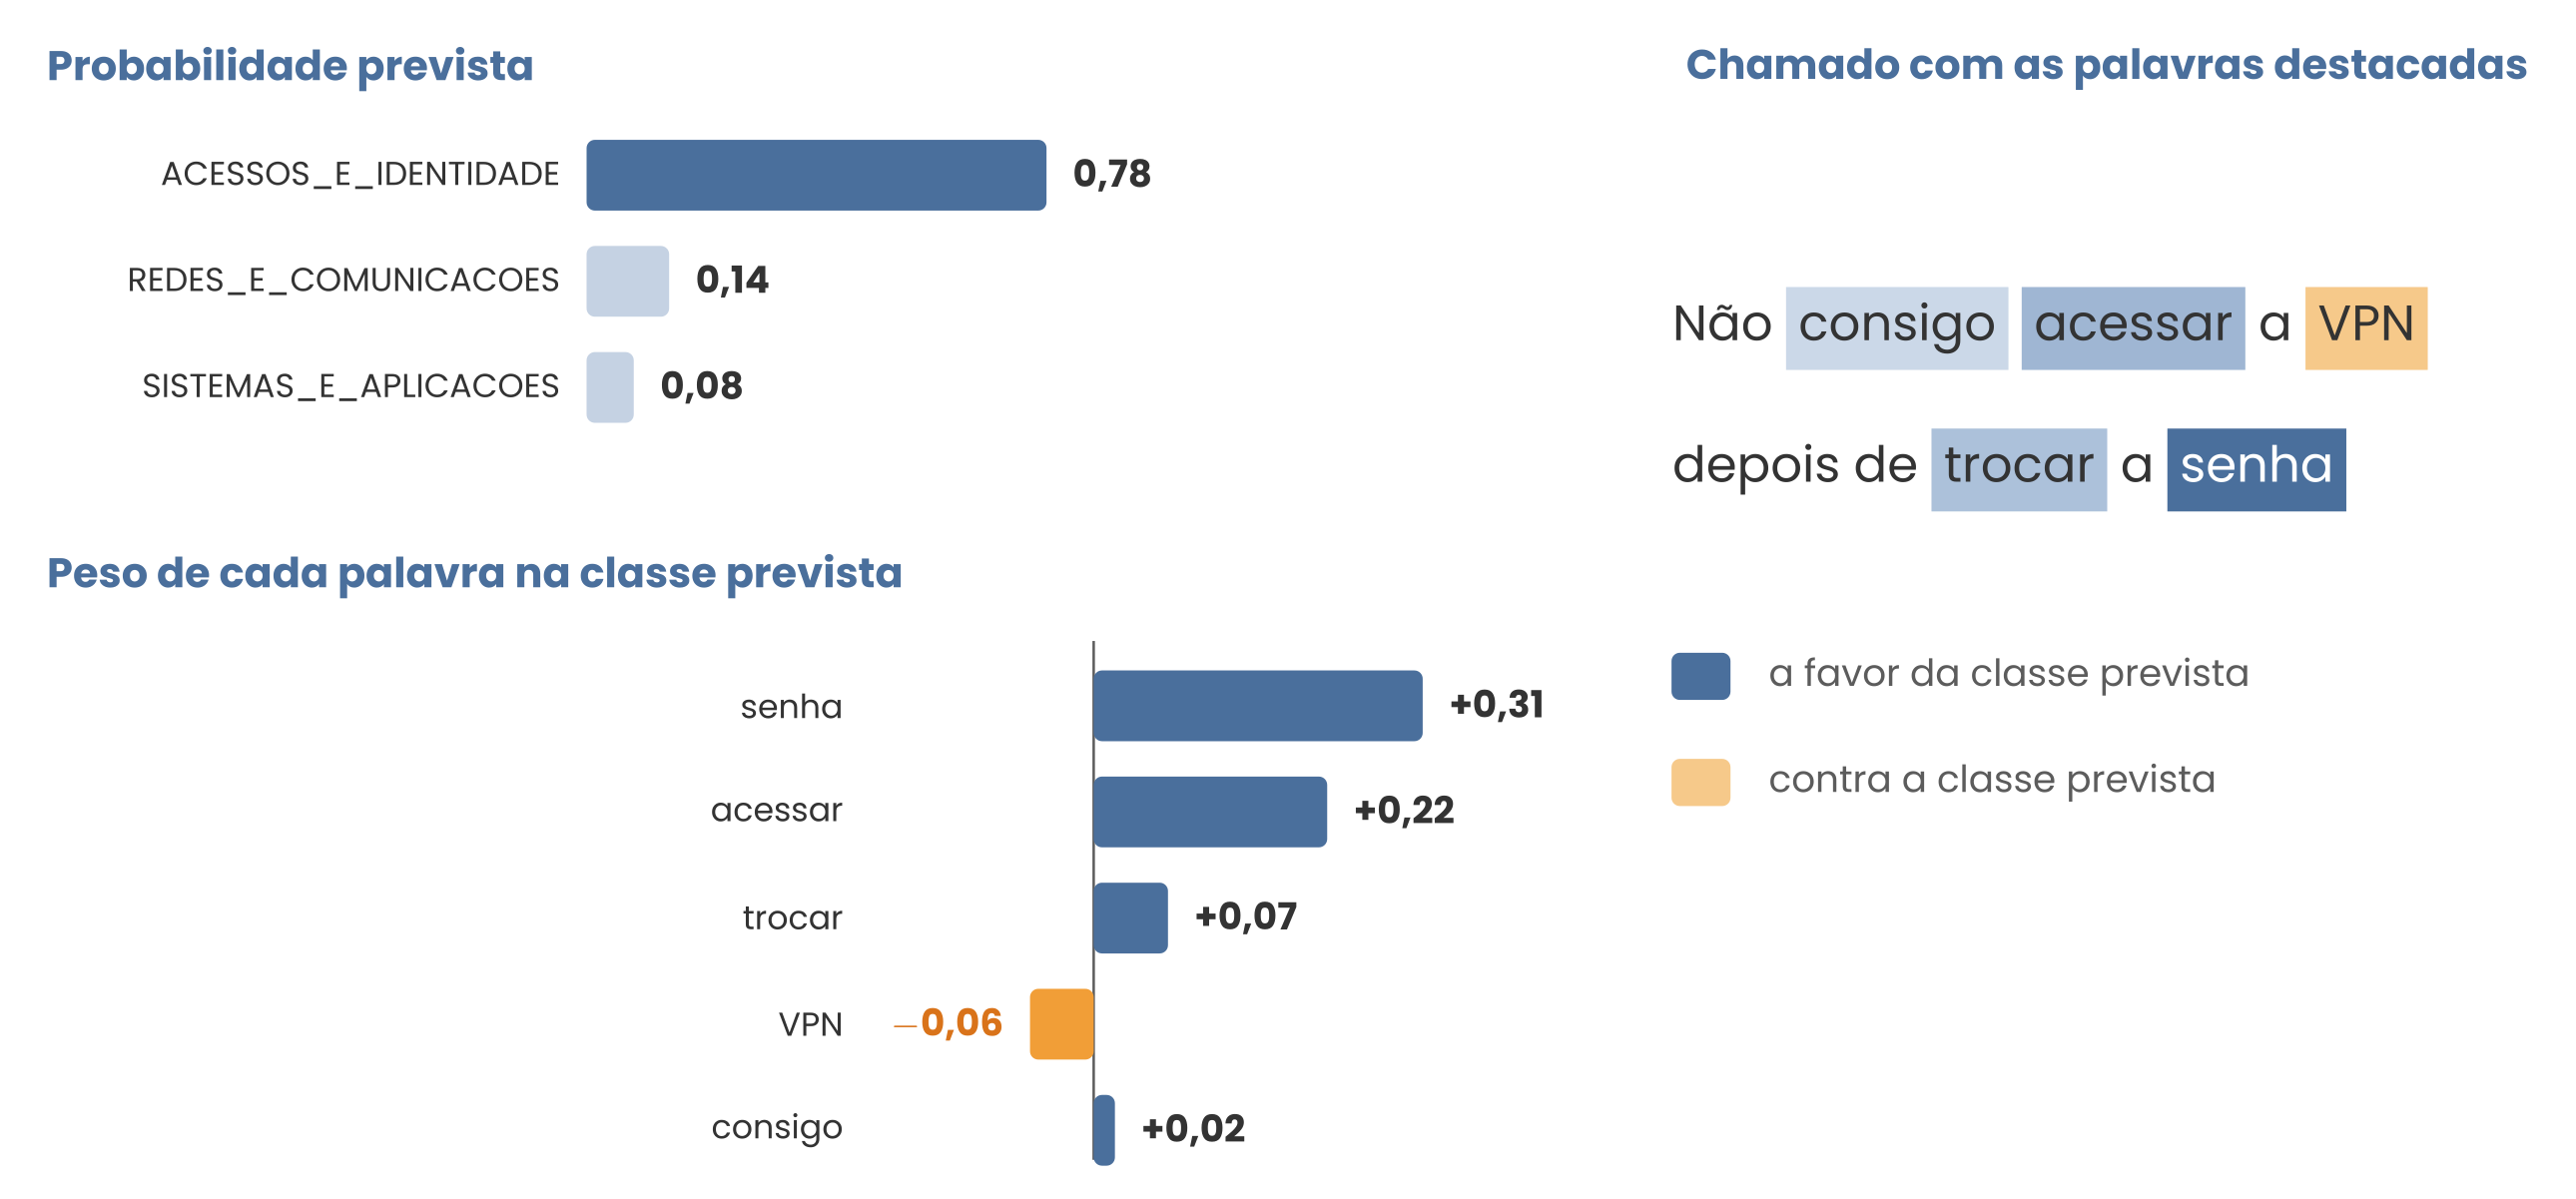
\includegraphics[width=\textwidth]{imagens/lime_exemplo_pt.png}
    \legend{Fonte: Adaptado de \citeonline{ribeiro2016}.\\ Nota: Valores ilustrativos, não extraídos de um modelo treinado.}
\end{figure}

% - - - - - - - - - - - - - - - - - - - - - - - - - - - - - - -
\subsubsubsection{Aplicação em classificação de texto}
\label{subsubsec:lime_texto}

No contexto de classificação de texto, cada palavra da entrada é tratada como uma \textit{feature}, ou seja, uma característica binária que indica se está presente ou ausente no texto. A explicação LIME indica quais palavras, quando presentes, aumentam a probabilidade de cada classe, e quais palavras a diminuem. O resultado pode ser visualizado como um destaque colorido sobre o texto original, onde palavras em azul contribuem positivamente para a classe predita e palavras em laranja contribuem negativamente.

\citeonline{mustafa2025} relataram que a aplicação de LIME na 
classificação de texto não apenas produz explicações úteis para o 
usuário final, mas também contribui para melhorar o processo de 
pré-processamento: ao revelar que \textit{stopwords}, palavras muito 
frequentes e de pouco conteúdo informativo, como artigos e preposições 
(``de'', ``o'', ``para''), recebem pesos desproporcionalmente altos 
nas explicações, o LIME evidenciou a necessidade de sua remoção.

% - - - - - - - - - - - - - - - - - - - - - - - - - - - - - - -
\subsubsubsection{Vantagens e limitações}
\label{subsubsec:lime_limitacoes}

A principal vantagem do LIME é sua generalidade: o método funciona com qualquer modelo e qualquer tipo de entrada sem necessidade de acesso ao interior do modelo. Isso o torna especialmente adequado para modelos de caixa-preta como o BERT, cujos mecanismos internos são de difícil interpretação direta.

Uma limitação a verificar é a estabilidade das explicações. O LIME gera as perturbações por amostragem aleatória \cite{ribeiro2016}. Embora os autores o descrevam como razoavelmente robusto ao ruído de amostragem, execuções diferentes sobre a mesma instância podem produzir explicações distintas. A colinearidade entre as \textit{features}, ou seja, quando algumas características extraídas do texto são muito parecidas ou carregam informações semelhantes, também afeta os pesos atribuídos \cite{salih2023}. Fixar a semente aleatória torna a explicação reprodutível, mas não garante a estabilidade: com outra semente, a explicação pode mudar.

\subsubsection{SHAP: \textit{SHapley Additive exPlanations}}
\label{subsec:shap}

% - - - - - - - - - - - - - - - - - - - - - - - - - - - - - - -
\subsubsubsection{Fundamentos: valores de Shapley da teoria dos jogos}
\label{subsubsec:shap_fundamentos}

SHAP foi proposto por \citeonline{lundberg2017} com base nos valores 
de Shapley da teoria dos jogos cooperativos. O problema que o SHAP 
resolve é: dada uma predição específica de um modelo, como distribuir 
o ``crédito'' por essa predição de forma justa entre as 
\textit{features} de entrada?

Na teoria dos jogos, o valor de Shapley de um jogador em um jogo 
cooperativo é calculado como a média ponderada de quanto cada jogador 
contribuiu individualmente em todas as combinações possíveis com os 
demais jogadores. \citeonline{lundberg2017} adaptam esse conceito 
para o contexto de modelos de aprendizado de máquina: cada 
\textit{feature} é um ``jogador'', a predição do modelo é o 
``valor do jogo'', e o valor SHAP de cada \textit{feature} mede 
o quanto ela contribuiu para a predição, considerando todas as 
possíveis ordens em que as \textit{features} poderiam ser incluídas.

Seja $F$ o conjunto das palavras distintas do campo explicado e $f_S(x_S)$ a probabilidade da classe prevista quando só as palavras de $S \subseteq F$ estão presentes (as demais são apagadas do texto, e não trocadas por um símbolo como \texttt{[MASK]}, e o outro campo fica fixo, com o texto original). O valor de Shapley da palavra $i$ é \cite{lundberg2017}:

\begin{equation}
\phi_i = \sum_{S \subseteq F \setminus \{i\}}
\frac{|S|!\,\big(|F| - |S| - 1\big)!}{|F|!}
\left[ f_{S \cup \{i\}}(x_{S \cup \{i\}}) - f_S(x_S) \right]
\label{eq:shapley}
\end{equation}

O termo entre colchetes é a \textbf{contribuição marginal} de $i$: quanto a probabilidade muda quando $i$ entra em um conjunto que já tem as palavras de $S$. O fator de peso é a \textbf{fração das $|F|!$ ordens possíveis de entrada das palavras em que exatamente as palavras de $S$ entram antes de $i$}: há $|S|!$ formas de ordenar as palavras de $S$ antes de $i$ e $(|F|-|S|-1)!$ formas de ordenar as restantes depois. Assim, $\phi_i$ é a média da contribuição marginal de $i$ sobre todas as ordens de entrada. Equivalentemente:

\begin{equation}
\phi_i = \frac{1}{|F|!} \sum_{\pi \in \Pi(F)}
\left[ f_{P_i^{\pi} \cup \{i\}}(x_{P_i^{\pi} \cup \{i\}}) - f_{P_i^{\pi}}(x_{P_i^{\pi}}) \right]
\label{eq:shapley-perm}
\end{equation}

em que $\Pi(F)$ é o conjunto das ordens (permutações) das palavras e $P_i^{\pi}$ são as palavras que vêm antes de $i$ na ordem $\pi$.

Considere um campo com três palavras, \textit{senha} ($s$), \textit{bloqueada} ($b$) e \textit{SAP} ($c$), e as probabilidades ilustrativas da Tabela~\ref{tab:exemplo_shap}.

\begin{table}[htb]
  \centering
  \caption{Probabilidades ilustrativas da classe ACESSOS\_E\_IDENTIDADE por conjunto de palavras presentes}
  \label{tab:exemplo_shap}
  \small
  \begin{tabular}{lcccccccc}
    \toprule
    $S$ & $\varnothing$ & $\{s\}$ & $\{b\}$ & $\{c\}$ & $\{s,b\}$ & $\{s,c\}$ & $\{b,c\}$ & $\{s,b,c\}$ \\
    \midrule
    $f_S(x_S)$ & 0,10 & 0,40 & 0,20 & 0,15 & 0,70 & 0,45 & 0,25 & 0,80 \\
    \bottomrule
  \end{tabular}
  \legend{Fonte: Elaborado pelos autores (valores ilustrativos).}
\end{table}

Com $|F| = 3$, os pesos são $1/3$ para $|S| = 0$, $1/6$ para cada $S$ com $|S| = 1$ e $1/3$ para $|S| = 2$, que somam 1. Para \textit{senha}:

\begin{equation}
\phi_s = \tfrac{1}{3}(0{,}40 - 0{,}10) + \tfrac{1}{6}(0{,}70 - 0{,}20)
       + \tfrac{1}{6}(0{,}45 - 0{,}15) + \tfrac{1}{3}(0{,}80 - 0{,}25) \approx 0{,}417
\label{eq:exemplo-shap}
\end{equation}

Da mesma forma, $\phi_b \approx 0{,}217$ e $\phi_c \approx 0{,}067$. A soma, $0{,}417 + 0{,}217 + 0{,}067 = 0{,}70$, é igual a $f_F(x_F) - f_\varnothing(x_\varnothing) = 0{,}80 - 0{,}10$, como garante a eficiência (Equação~\ref{eq:eficiencia}). \textit{Senha} é a palavra que mais contribui, porque eleva a probabilidade em qualquer conjunto em que entra.

A Figura~\ref{fig:shap_exemplo} ilustra esse conceito: cada 
\textit{feature} desloca a predição do valor base até o 
valor final do modelo.

\begin{figure}[H]
    \caption{Representação dos valores SHAP por \textit{feature}}
    \label{fig:shap_exemplo}
    \centering
    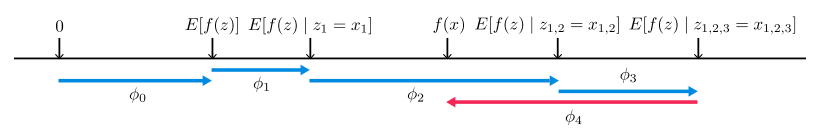
\includegraphics[width=0.75\textwidth]{imagens/shap_exemplo.png}
    \legend{Fonte: \citeonline{lundberg2017}.}
\end{figure}

% - - - - - - - - - - - - - - - - - - - - - - - - - - - - - - -
\subsubsubsection{Propriedades matemáticas: eficiência, simetria e ausência}
\label{subsubsec:shap_propriedades}

A formulação baseada em valores de Shapley garante ao SHAP propriedades matemáticas desejáveis, que o distinguem de métodos \textit{ad hoc} de atribuição de importância. \citeonline{lundberg2017} formulam essas propriedades como acurácia local, ausência (\textit{missingness}) e consistência, que se relacionam aos axiomas clássicos de Shapley de eficiência, jogador nulo e monotonicidade. Na forma clássica dos axiomas de Shapley, as propriedades de interesse aqui são três.

\textbf{Eficiência (acurácia local):}

\begin{equation}
\sum_{i \in F} \phi_i = f_F(x_F) - f_\varnothing(x_\varnothing) = f(x) - \phi_0
\label{eq:eficiencia}
\end{equation}

A soma dos valores é a diferença entre a predição para o chamado, $f(x)$, e o valor-base $\phi_0 = f_\varnothing(x_\varnothing)$. Os valores SHAP positivos contribuem para a classe predita e os negativos contribuem contra ela. Aqui, $\phi_0$ é a probabilidade da classe prevista sem nenhuma palavra do campo explicado e com o outro campo fixo, e não a predição média sobre o conjunto de dados.

\textbf{Simetria:} se $f_{S \cup \{i\}}(x_{S \cup \{i\}}) = f_{S \cup \{j\}}(x_{S \cup \{j\}})$ para todo $S$ sem $i$ e $j$, então $\phi_i = \phi_j$.

\textbf{Ausência (jogador nulo):} se $f_{S \cup \{i\}}(x_{S \cup \{i\}}) = f_S(x_S)$ para todo $S$, então $\phi_i = 0$.

Essas propriedades conferem ao SHAP uma fundamentação teórica sólida que o LIME não possui, o que dá ao SHAP garantias teóricas quando calculado de forma exata; quando estimado por amostragem de permutações, a eficiência e a ausência continuam valendo, e a simetria vale apenas em média.

% - - - - - - - - - - - - - - - - - - - - - - - - - - - - - - -
\subsubsubsection{Cálculo do SHAP em modelos de texto}
\label{subsubsec:shap_kernel}

O cálculo exato pela Equação~\ref{eq:shapley} exige avaliar o modelo em todos os subconjuntos de palavras:

\begin{equation}
\text{avaliações no cálculo exato} = 2^{|F|}, \qquad 2^{10} = 1{.}024
\label{eq:custo-shap}
\end{equation}

e o número dobra a cada palavra a mais. Por isso, nos campos com mais de 10 palavras distintas, o valor foi estimado pelo explicador de permutações da biblioteca \textit{shap}. Sorteiam-se $M$ permutações e cada uma é percorrida nos dois sentidos; a média é sobre as $2M$ ordens: % CONFERIDO: shap.explainers.Permutation, cada permutacao nos dois sentidos, divisao por 2M. Orcamento 2.000 em shap_chamados.py.

\begin{equation}
\hat{\phi}_i = \frac{1}{2M} \sum_{m=1}^{M}
\left[ \Delta_i^{\rightarrow}(m) + \Delta_i^{\leftarrow}(m) \right]
\label{eq:shap-amostragem}
\end{equation}

em que $\Delta_i^{\rightarrow}(m)$ é a contribuição da palavra $i$ na ordem sorteada e $\Delta_i^{\leftarrow}(m)$ é a contribuição na ordem inversa. O orçamento foi de 2.000 avaliações do modelo por campo. Como cada permutação, percorrida nos dois sentidos, custa $2|F| + 1$ avaliações, o número de permutações é:

\begin{equation}
M = \left\lfloor \frac{2000}{2\,|F| + 1} \right\rfloor, \qquad |F| = 30 \;\Rightarrow\; M = 32
\label{eq:orcamento}
\end{equation}

o que explica a variação entre repetições observada na Seção~\ref{subsubsec:res_estabilidade}. O \textit{KernelSHAP} \cite{lundberg2017} é outra forma de estimar esses valores, mas não foi adotado: como a amostragem de permutações já estima os mesmos valores de Shapley, o grupo decidiu não incluir um segundo estimador, por não haver vantagem que justificasse sua adoção.

\subsubsection{Comparação entre SHAP e LIME}
\label{subsec:shap_lime}

% - - - - - - - - - - - - - - - - - - - - - - - - - - - - - - -
\subsubsubsection{Consistência e estabilidade das explicações}
\label{subsubsec:comparacao_consistencia}

\citeonline{salih2023} realizaram uma análise comparativa entre SHAP e LIME, discutindo suas propriedades e seu comportamento em um estudo de caso de classificação com dados tabulares. Em termos de estabilidade, os autores avaliam a lista de variáveis informativas entre diferentes modelos e mostram que os dois métodos são fortemente afetados pelo modelo adotado e pela colinearidade entre as \textit{features}. Quanto à estabilidade entre execuções repetidas, espera-se que o SHAP, por ser baseado em uma formulação matemática única com garantias teóricas \cite{lundberg2017}, seja menos sensível à aleatoriedade do processo de amostragem, enquanto o LIME depende de perturbações aleatórias e de um ajuste local \cite{ribeiro2016}, o que pode levar a explicações distintas para a mesma instância em execuções diferentes.

Com base nessas propriedades, espera-se que o SHAP seja preferível quando a consistência e a fundamentação teórica das explicações são prioritárias, enquanto o LIME possa ser preferível quando a velocidade de geração das explicações é mais importante do que a estabilidade. Essa expectativa é examinada na Seção~\ref{subsubsec:res_estabilidade}.

% - - - - - - - - - - - - - - - - - - - - - - - - - - - - - - -
\subsubsubsection{Custo computacional}
\label{subsubsec:comparacao_custo}

O custo do LIME é fixo, definido pelo número de perturbações. O do SHAP cresce com o número de palavras: o cálculo exato exige $2^n$ avaliações para $n$ palavras (1.024 para 10 palavras) e, acima de certo tamanho, é preciso estimar por amostragem, com um orçamento de avaliações definido.
% - - - - - - - - - - - - - - - - - - - - - - - - - - - - - - -
\subsubsubsection{Justificativa para uso conjunto neste trabalho}
\label{subsubsec:comparacao_justificativa}

A decisão de implementar e comparar SHAP e LIME neste trabalho, em vez de escolher apenas um dos métodos, é fundamentada em duas razões. Primeiro, a comparação entre os dois métodos produz evidência empírica sobre a qualidade e consistência das explicações geradas para chamados de TI em PT-BR, contribuição metodológica relevante para a literatura sobre XAI em domínios especializados. Segundo, a construção do grafo de co-ocorrência proposto utiliza os valores SHAP e LIME como pesos dos nós (as palavras) de um grafo de co-ocorrência, rede em que cada nó é uma palavra e cada aresta liga palavras que aparecem próximas no texto, permitindo avaliar 
se a escolha do método de XAI afeta a estrutura do grafo resultante.

\subsubsection{XAI aplicado a classificação de texto e chamados de TI}
\label{subsec:xai_aplicado}

% - - - - - - - - - - - - - - - - - - - - - - - - - - - - - - -
\subsubsubsection{LIME em classificação multiclasse de texto}
\label{subsubsec:xai_mustafa}

\citeonline{mustafa2025} propuseram um \textit{framework} de 
classificação de texto que combina PLN e XAI. O sistema inclui 
pré-processamento com NLTK (\textit{Natural Language Toolkit} -- Kit de Ferramentas de Linguagem Natural), 
balanceamento de classes com SMOTE (\textit{Synthetic Minority Oversampling Technique} -- Técnica de Sobreamostragem Sintética de Minorias), 
técnica que cria exemplos sintéticos das classes minoritárias a partir da interpolação 
entre exemplos vizinhos, para lidar com \textit{datasets} desbalanceados, 
e validação cruzada estratificada repetida: uma técnica que divide 
os dados em múltiplos subconjuntos para avaliar o modelo de forma 
mais robusta, garantindo que todas as classes estejam representadas 
em cada divisão. O modelo utilizado foi um híbrido de regressão 
\textit{ridge} com regressão logística. O LIME foi utilizado para ilustrar a explicabilidade das
classificações em um estudo de caso com texto médico; o
conjunto de dados reúne textos de seis classes: medicina,
esportes, entretenimento, política, tecnologia e negócios. Após o ajuste do pré-processamento, a acurácia de alguns modelos individuais subiu de 0,43 para 0,64 (\textit{Linear Discriminant Analysis}) e de 0,51 para 0,59 (\textit{AdaBoost}), e o modelo híbrido atingiu até 99\% de acurácia, em um conjunto combinado de 2.494 textos.

O trabalho demonstra que a integração de XAI ao \textit{pipeline} 
de classificação não é apenas uma camada de interpretabilidade 
adicionada ao final do processo, mas pode também influenciar 
decisões de pré-processamento e seleção de \textit{features}, 
melhorando a qualidade do modelo como um todo.

% - - - - - - - - - - - - - - - - - - - - - - - - - - - - - - -
\subsubsubsection{SHAP e LIME em ambiente ITSM corporativo}
\label{subsubsec:xai_razma}

\citeonline{razma2026} aplicaram o LIME à regressão logística com \textit{TF-IDF} e ao mBERT \textit{fine-tuned}, e o SHAP à regressão logística, em um ambiente ITSM corporativo real. Os resultados qualitativos das explicações foram bem distintos: o modelo linear tendia a destacar palavras-chave literais com alta frequência no corpus, enquanto o BERT destacava termos semanticamente coerentes com o significado do chamado.

Essa diferença qualitativa, observada por \citeonline{razma2026} com o mBERT, motiva verificar se o BERTimbau, combinado com SHAP e LIME, também destaca termos coerentes com a categoria, o que é examinado nos casos aplicados (Seção~\ref{subsec:res_casos}).

\subsubsection{Auditabilidade}
\label{subsec:auditabilidade}

A literatura de XAI não apresenta uma definição única e consolidada de
auditabilidade. Por essa razão, adota-se aqui uma definição operacional,
construída a partir de propriedades já estabelecidas na literatura: um
sistema de classificação é auditável quando permite rastrear, verificar
e reproduzir a explicação de cada decisão do modelo. Trata-se, portanto,
de uma propriedade técnica do sistema, e não da confiança percebida por
quem o utiliza. Essa distinção é relevante porque o estudo de \citeonline{zemp2021}, 
ao relatar a reação de analistas de suporte a um sistema de classificação 
em produção, trata da aceitação pela equipe, e não da propriedade técnica definida aqui.

A definição se desdobra em três dimensões:

\begin{itemize}
    \item \textbf{Rastreabilidade}: a capacidade de atribuir a decisão
    do modelo a termos específicos da entrada, obtida por meio dos
    valores SHAP \cite{lundberg2017} e LIME \cite{ribeiro2016};

    \item \textbf{Estabilidade}: a reprodutibilidade da explicação
    gerada para uma mesma instância ao longo de execuções repetidas,
    questão especialmente relevante para o LIME, que depende de
    amostragem aleatória de perturbações \cite{ribeiro2016};

    \item \textbf{Fidelidade}: o grau em que a explicação reflete o
    processo de decisão efetivamente utilizado pelo modelo
    \cite{jacovi2020}, verificável pela variação da confiança preditiva
    ao remover da entrada os termos apontados como mais relevantes.
\end{itemize}

Neste trabalho, a rastreabilidade é avaliada no grafo (cenário D), e a fidelidade e a estabilidade, nas explicações SHAP e LIME (cenário C).

A validação da percepção de confiança por parte de gestores ou analistas
de TI não é objeto deste trabalho, sendo reconhecida como extensão
natural da pesquisa.

% ---------------------------------------------------------------
\subsection{Grafos de co-ocorrência como representação estrutural de texto}

Um grafo de co-ocorrência é uma estrutura $G = (V, E, W, f_{\text{shap}}, f_{\text{lime}})$, adaptada de \citeonline{yao2019} com a inclusão das funções de peso dos nós $f_{\text{shap}}$ e $f_{\text{lime}}$, proposta deste trabalho. 

\subsubsection{Fundamentos de grafos aplicados a texto}
\label{subsec:grafos_fundamentos}

% - - - - - - - - - - - - - - - - - - - - - - - - - - - - - - -
\subsubsubsection{Grafo de co-ocorrência: nós, arestas e janela deslizante}
\label{subsubsec:grafos_definicao}

Na estrutura $G = (V, E, W, f_{\text{shap}}, f_{\text{lime}})$ apresentada acima:

\begin{itemize}
    \item $V$ representa o conjunto de nós, correspondendo às
    palavras únicas do texto;
    
    \item $E$ representa o conjunto de arestas, conectando pares 
    de palavras que co-ocorrem dentro de uma janela 
    deslizante de tamanho $w$;
    
    \item $W$ representa os pesos das arestas, determinados pela 
    frequência de co-ocorrência entre as palavras;
    
    \item $f_{\text{shap}}$ representa os pesos dos nós calculados 
    pelo método SHAP, indicando a contribuição de cada 
    palavra para a predição do modelo \cite{lundberg2017};
    
    \item $f_{\text{lime}}$ representa os pesos dos nós calculados 
    pelo método LIME, permitindo comparação visual entre os dois 
    métodos de explicabilidade \cite{ribeiro2016}.
\end{itemize}

A janela deslizante \cite{yao2019} percorre o texto posição por posição; em cada posição, todos os pares de palavras dentro da janela recebem uma aresta ou têm o peso de sua aresta existente incrementado. Essa representação captura informação 
estrutural sobre o texto que as representações vetoriais não 
preservam: duas palavras que frequentemente aparecem juntas 
no mesmo contexto estarão conectadas por uma aresta de alto peso 
no grafo, independentemente de sua posição absoluta na sequência. 
Para chamados de TI, isso significa que termos técnicos que tendem 
a co-ocorrer em chamados de uma mesma categoria, como ``VPN'' e 
``acesso'' em chamados de conectividade, estarão estruturalmente 
próximos no grafo, com pesos de nós proporcionais à sua 
importância explicativa calculada por SHAP e LIME.

Seja o texto do chamado, depois da remoção das \textit{stopwords}, a sequência de palavras $t_1, \dots, t_n$, e $w$ o tamanho da janela. O peso da aresta entre duas palavras distintas $a \neq b$ é o número de janelas que contêm as duas:

\begin{equation}
W(a,b) = \sum_{k=1}^{n-w+1} \mathbf{1}\Big[ a \in \{t_k, \dots, t_{k+w-1}\} \;\wedge\; b \in \{t_k, \dots, t_{k+w-1}\} \Big]
\label{eq:aresta}
\end{equation}

O peso do nó $v$ para o método $m \in \{\mathrm{SHAP}, \mathrm{LIME}\}$ é o módulo da soma dos pesos de suas ocorrências, e o sinal define a cor:

\begin{equation}
f_m(v) = \Bigg| \sum_{j:\, t_j = v} \phi_j^{(m)} \Bigg|, \qquad
\mathrm{cor}(v) =
\begin{cases}
\text{azul}, & \sum_{j:\, t_j = v} \phi_j^{(m)} \ge 0 \\
\text{laranja}, & \text{caso contrário}
\end{cases}
\label{eq:no}
\end{equation}

O conjunto de arestas é $E = \{(a,b) : W(a,b) > 0\}$.

A Figura~\ref{fig:grafo_exemplo} ilustra a construção com o mesmo chamado fictício da Figura~\ref{fig:lime_exemplo}. À esquerda, estão as palavras que restam depois da remoção das palavras vazias (\textit{stopwords}) e as duas janelas de tamanho 4 que percorrem o texto. À direita, está o grafo resultante: o tamanho de cada nó é proporcional ao módulo do peso da palavra, e o número sobre a aresta indica em quantas janelas o par aparece junto.

\begin{figure}[H]
    \caption{Construção de um grafo de co-ocorrência a partir de um chamado fictício}
    \label{fig:grafo_exemplo}
    \centering
    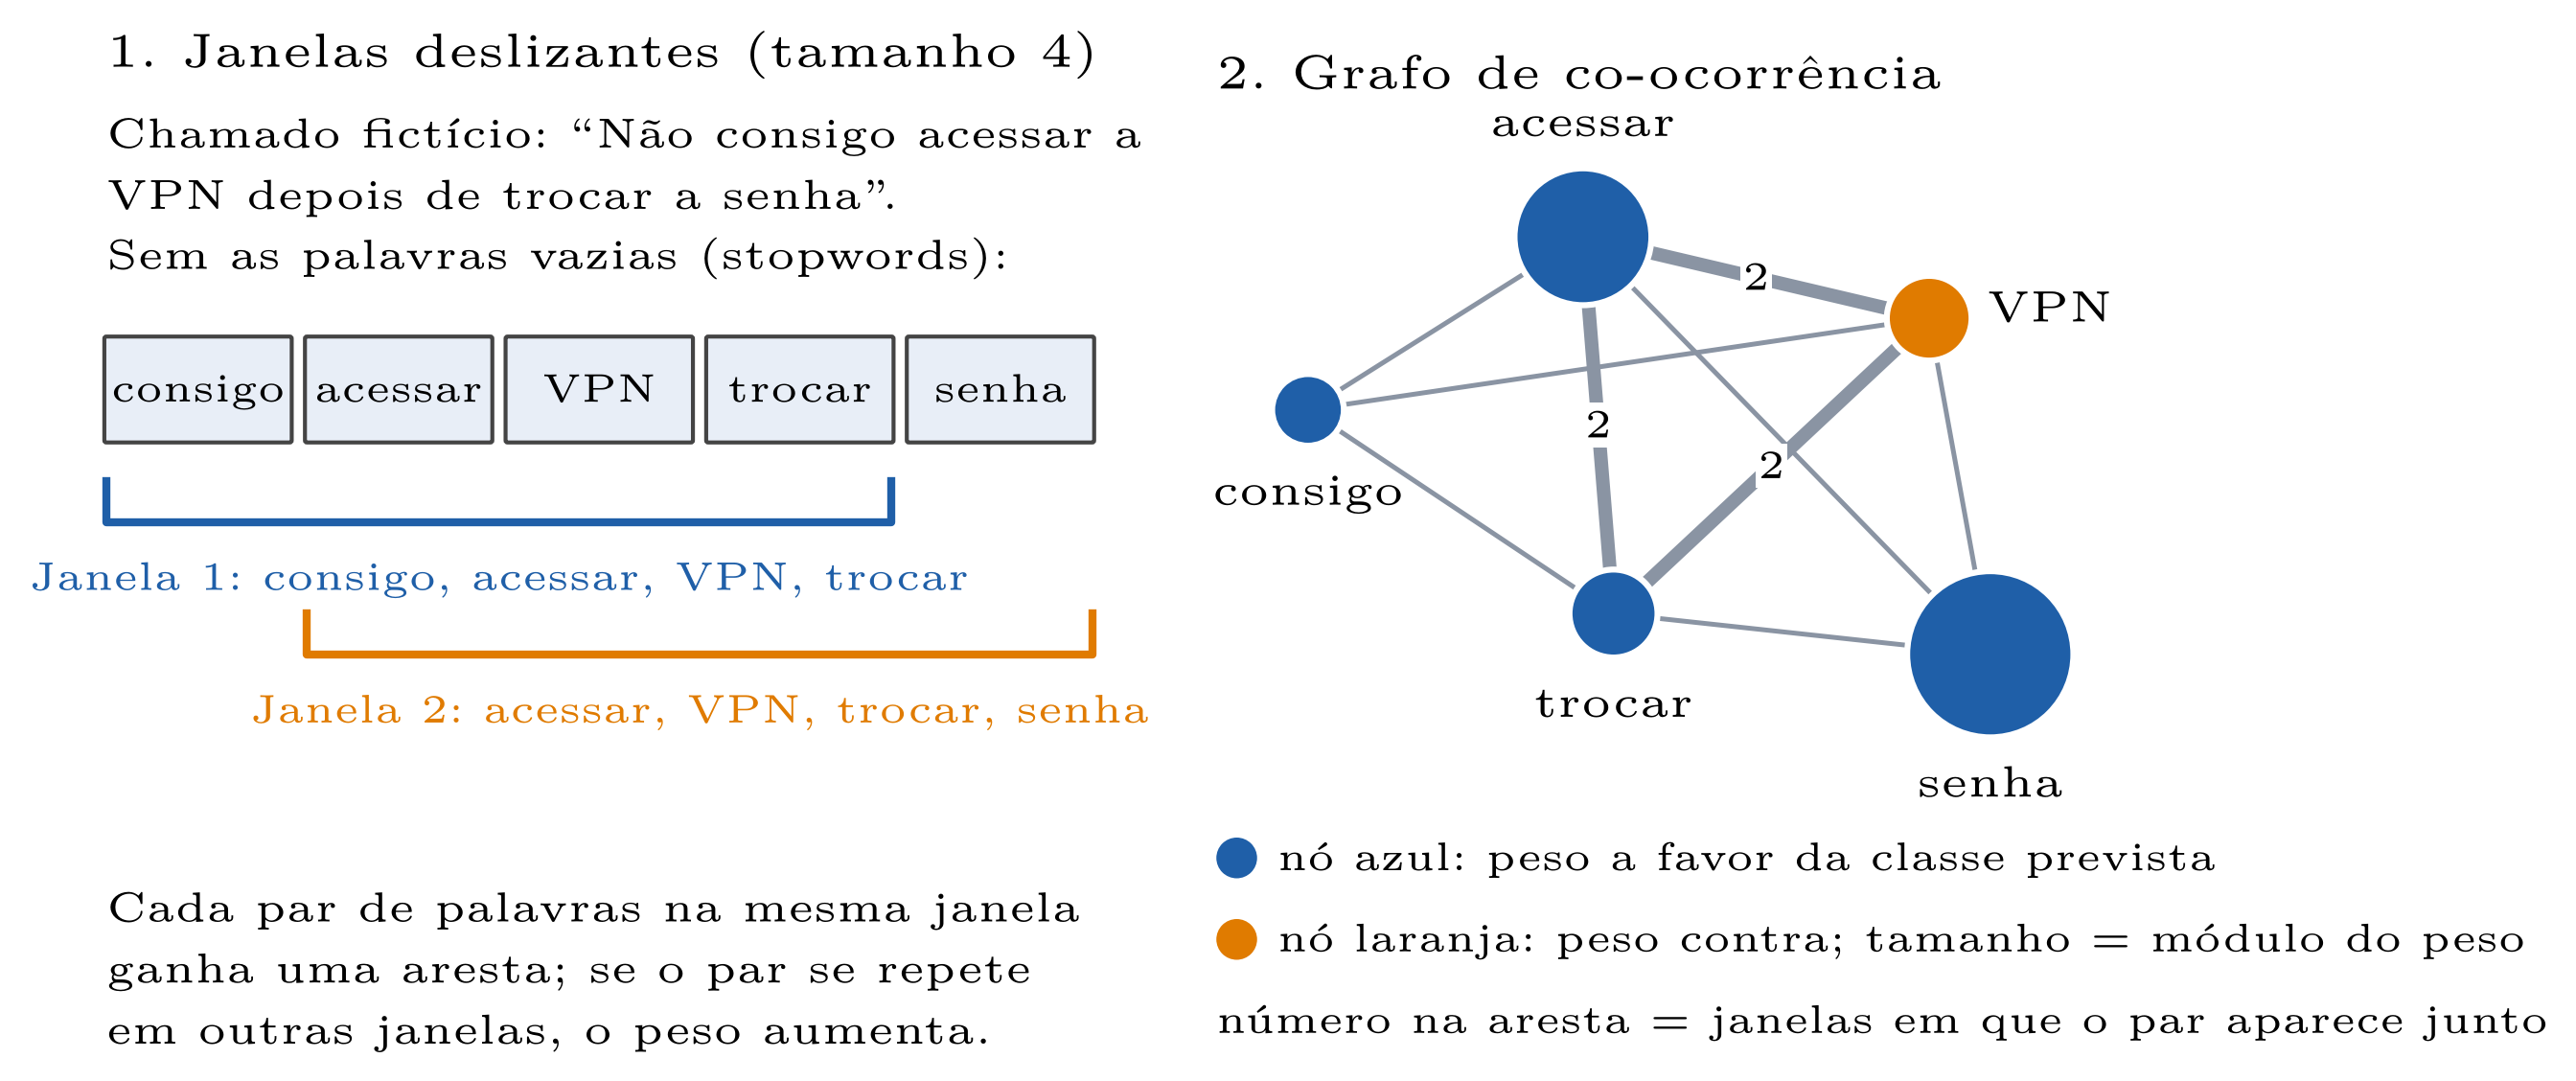
\includegraphics[width=\textwidth]{imagens/grafo_cooc_exemplo.png}
    \legend{Fonte: Elaborado pelos autores.\\ Nota: Valores ilustrativos, não extraídos de um modelo treinado.}
\end{figure}
% - - - - - - - - - - - - - - - - - - - - - - - - - - - - - - -
\subsubsubsection{Ponderação de arestas: frequência e PMI}
\label{subsubsec:grafos_ponderacao}

O peso das arestas em um grafo de co-ocorrência pode ser determinado por diferentes métricas. A abordagem mais simples utiliza a frequência bruta de co-ocorrência, ou seja, a contagem de quantas vezes o par de palavras co-ocorreu dentro da janela deslizante. Métricas mais sofisticadas, como a PMI (\textit{Pointwise Mutual Information} -- Informação Mútua Pontual), normalizam a frequência de co-ocorrência pelas frequências individuais de cada palavra, favorecendo pares que co-ocorrem mais do que seria esperado pelo acaso \cite{yao2019}.

A PMI de um par de palavras $a$ e $b$ é
\begin{equation}
\text{PMI}(a,b) = \log\frac{p(a,b)}{p(a)\,p(b)}
\end{equation}
onde $p(a,b)$ é a fração de janelas em que $a$ e $b$ aparecem juntos, e $p(a)$ e $p(b)$ são as frações de janelas em que cada um aparece. A frequência de co-ocorrência é, portanto, normalizada pelas frequências individuais das palavras: um par só recebe PMI alta se aparecer junto mais do que o esperado se os termos fossem independentes.

\subsubsection{\textit{TextGCN}: formalização do grafo de co-ocorrência}
\label{subsec:textgcn}

% - - - - - - - - - - - - - - - - - - - - - - - - - - - - - - -
\subsubsubsection{Grafo heterogêneo documento-palavra}
\label{subsubsec:textgcn_grafo}

\citeonline{yao2019} propuseram o \textit{TextGCN} (\textit{Text Graph Convolutional Network}), modelo que constrói um único grafo heterogêneo para todo o corpus, conectando documentos e palavras. As arestas documento-palavra recebem pesos baseados em TF-IDF, refletindo a importância de cada palavra para cada documento. As arestas palavra-palavra recebem pesos baseados em PMI calculada sobre co-ocorrências em janela deslizante de tamanho 20 sobre todo o corpus, refletindo a força de associação semântica entre pares de palavras.

Essa estrutura permite que as GCN (\textit{Graph Convolutional Network} -- Rede Neural Convolucional em Grafos) propaguem informação simultaneamente entre documentos e palavras, capturando relações semânticas globais que modelos baseados em sequências não conseguem representar diretamente.

% - - - - - - - - - - - - - - - - - - - - - - - - - - - - - - -
\subsubsubsection{Redes neurais de grafos e propagação de informação}
\label{subsubsec:textgcn_gcn}

As GNN (\textit{Graph Neural Network} -- Rede Neural de Grafos) operam sobre grafos propagando informação entre nós vizinhos por meio de operações de agregação e transformação. Em cada camada da rede, a representação de cada nó é atualizada com base nas representações de seus vizinhos na iteração anterior \cite{yao2019}. Após múltiplas camadas, cada nó possui uma representação que agrega informação de sua vizinhança local de múltiplos saltos. Nas GCN, a atualização é dada por:

\begin{equation}
L^{(j+1)} = \rho\!\left( \tilde{A}\, L^{(j)}\, W_j \right), \qquad
\tilde{A} = D^{-\frac{1}{2}} A\, D^{-\frac{1}{2}}
\label{eq:gcn}
\end{equation}

em que $A$ é a matriz de adjacência do grafo, com a diagonal igual a 1 (laços próprios), $D$ a matriz diagonal de graus de $A$, $\tilde A$ a matriz de adjacência normalizada, $L^{(j)}$ as representações dos nós na camada $j$ (com $L^{(0)} = X$), $W_j$ os pesos aprendidos e $\rho$ uma função de ativação \cite{yao2019}.

A relevância do \textit{TextGCN} é fundamentalmente teórica: ele formaliza matematicamente a estrutura do grafo de co-ocorrência e demonstra sua utilidade para classificação de texto.

\subsubsection{Combinação de BERT com grafos de co-ocorrência}
\label{subsec:bert_grafo}

% - - - - - - - - - - - - - - - - - - - - - - - - - - - - - - -
\subsubsubsection{\textit{Embeddings} BERT como \textit{features} iniciais dos nós}
\label{subsubsec:bert_grafo_embeddings}

\citeonline{yang2021} propuseram o BEGNN (\textit{BERT-Enhanced Text Graph Neural Network} -- Rede Neural de Grafos de Texto Aprimorada por BERT), que combina representações contextualizadas do BERT com grafos de co-ocorrência para classificação de texto. Na arquitetura BEGNN, um grafo de co-ocorrência é construído separadamente para cada documento, com janela deslizante de tamanho 3, e seus nós são inicializados com vetores GloVe; uma rede neural de grafos com portas (\textit{Gated Graph Neural Network}) propaga informação entre nós vizinhos, produzindo características estruturais de cada palavra. Em paralelo, o BERT, ajustado à tarefa (\textit{fine-tuning}), produz características semânticas das palavras. As duas representações interagem em uma camada de co-atenção e são agregadas (por \textit{max-pooling}, concatenação ou soma), e uma camada totalmente conectada prediz a categoria.

Essa combinação aborda uma limitação do BERT quando utilizado isoladamente: o mecanismo de atenção do BERT captura relações entre \textit{tokens}, mas essas relações são implícitas nos pesos de atenção e não explicitamente estruturadas como um grafo. O grafo de co-ocorrência fornece uma estrutura explícita que complementa as representações contextualizadas.

% - - - - - - - - - - - - - - - - - - - - - - - - - - - - - - -
\subsubsubsection{Resultados em vocabulário técnico especializado}
\label{subsubsec:bert_grafo_resultados}

\citeonline{yang2021} avaliaram o BEGNN em múltiplos \textit{datasets} de classificação de texto, demonstrando que a combinação BERT + grafo supera o \textit{TextGCN} nas quatro bases avaliadas, inclusive em uma base de resumos médicos (Ohsumed); segundo os autores, o ganho é mais evidente nos textos mais longos. Esse resultado é relevante para o presente trabalho porque sugere que a estrutura de grafo de co-ocorrência captura informação complementar às representações do BERT, como as do BERTimbau.

\subsubsection{Grafo de co-ocorrência combinado com XAI}
\label{subsec:grafo_xai}

% - - - - - - - - - - - - - - - - - - - - - - - - - - - - - - -
\subsubsubsection{Ponderação de nós por \textit{scores} de explicabilidade}
\label{subsubsec:grafo_xai_ponderacao}

\citeonline{talebi2025} apresentam o trabalho de maior proximidade 
metodológica com o presente Trabalho de Conclusão de Curso (TCC): aplicam o Psycho-RoBERTa (um RoBERTa pré-treinado em textos psicológicos) combinado com LIME 
e um grafo de co-ocorrência para detectar \textit{body shaming}, 
prática de humilhar pessoas com base em sua aparência física, em 
redes sociais em inglês. No trabalho de \citeonline{talebi2025}, o grafo de co-ocorrência é construído com nós representando termos e arestas ponderadas pelo número de textos em que os dois termos aparecem juntos. Os termos de maior importância LIME são comparados com os nós centrais do grafo, com os quais coincidem de perto, mas os \textit{scores} do LIME não são usados como pesos do grafo.

O presente trabalho adotou uma abordagem análoga, mas com diferenças importantes: utilizou o BERTimbau em vez do RoBERTa, aplicou os valores SHAP e LIME como pesos dos nós, enquanto \citeonline{talebi2025} usam o LIME apenas para comparação com o grafo, e o domínio de aplicação foi a classificação de chamados de suporte de TI em português brasileiro. A escolha de ponderar os nós reflete a intenção de destacar visualmente as palavras individualmente mais relevantes para a predição, enquanto as arestas mantêm sua função de representar a estrutura de co-ocorrência do texto.

% - - - - - - - - - - - - - - - - - - - - - - - - - - - - - - -
\subsubsubsection{Visualização interativa como camada de auditabilidade}
\label{subsubsec:grafo_xai_visualizacao}

Neste trabalho, a combinação de grafos de co-ocorrência com \textit{scores} de explicabilidade é exibida em uma interface interativa que torna o processo decisório auditável. Nessa abordagem, os nós 
do grafo são dimensionados proporcionalmente à importância de cada 
palavra calculada pelo método XAI, e as arestas são ponderadas 
pela frequência de co-ocorrência, produzindo uma representação visual 
que combina estrutura relacional do texto com relevância explicativa 
do modelo.

Essa camada de visualização tem o potencial de transformar a saída 
opaca do modelo em uma representação auditável, o que responde a uma limitação dos classificadores opacos: sem acesso às razões da decisão, fica difícil para os analistas de suporte avaliar o comportamento do modelo e decidir se confiam nele \cite{ribeiro2016}. O presente trabalho avalia a 
propriedade técnica de auditabilidade da representação proposta, sem 
medir a adoção efetiva do sistema por usuários. Sua implementação é detalhada no Capítulo~\ref{cap:desenvolvimento}.

% ---------------------------------------------------------------
\section{Trabalhos correlatos}
\label{sec:trabalhos_relacionados}

Os quatro trabalhos a seguir enfrentaram o desafio de automatizar a triagem de chamados de suporte, servindo de base comparativa para a evolução proposta neste TCC.

\subsection{Trabalho 1: Text Classification of Service Desk Tickets}

\citeonline{zemp2021} abordou o problema da triagem automática em um ambiente corporativo. 
Para resolvê-lo, o autor comparou modelos CNN, BiLSTM e RoBERTa. A CNN alcançou 92\% de acurácia de validação. O estudo é detalhado na Seção~\ref{subsubsec:helpdesk_caixapreta}. O presente trabalho 
diferencia-se por focar na explicabilidade via SHAP, LIME e grafos, permitindo que os analistas de TI 
entendam o ``porquê'' da classificação.

\subsection{Trabalho 2: A Hybrid Continual Machine Learning Model for Efficient Hierarchical Classification of Domain-Specific Text in The Presence of Class Overlap (Case Study: IT Support Tickets)}

\citeonline{wahba2023} enfrentou o mesmo desafio de classificação de chamados, 
mas propôs uma abordagem focada em eficiência para domínios especializados. 
A solução utilizou um modelo híbrido (HOOM, \textit{Hybrid Online Offline Model} -- Modelo Híbrido \textit{Online} e \textit{Offline}) que combina um SVM linear e regras definidas com especialistas a um classificador \textit{online}, que se atualiza a cada nova amostra (detalhado na Seção~\ref{subsubsec:helpdesk_debate}). A metodologia 
demonstrou que em textos técnicos, modelos mais simples podem ser competitivos: 
a autora testou BERT e XLM (\textit{Cross-lingual Language Model} -- Modelo de Linguagem Multilíngue) e não encontrou ganho significativo sobre o SVM linear. 
Os resultados mostraram bom desempenho com baixo custo computacional. A limitação, 
em relação a este trabalho, é que a tese usa dados em inglês, não públicos, e não 
avalia explicações por palavra com métodos como SHAP e LIME. O presente trabalho 
adotou o BERTimbau, específico para PT-BR, que captura o contexto das palavras, 
e o combinou com SHAP, LIME e visualização em grafos para explicar as classificações.

\subsection{Trabalho 3: Aprendizado de máquina baseado em Classificação hierárquica de textos aplicado ao contexto chamados de suporte}

\citeonline{yokota2025} investigou a classificação de chamados de atendimento ao cliente especificamente em português brasileiro, utilizando \textit{Naive Bayes} e MLP sobre \textit{embeddings} do Multilingual E5. A metodologia focou na estrutura hierárquica das categorias (31 categorias e 240 subcategorias). Os resultados apresentaram F1-macro limitado, no máximo 61\%. A lacuna principal foi o desempenho baixo dos classificadores, que a autora associa ao desbalanceamento, à proximidade semântica entre categorias e ao vocabulário especializado, sem tratar da explicabilidade das decisões. O presente trabalho diferencia-se pelo ajuste fino de uma arquitetura de estado da arte (BERTimbau) pré-treinada em português e pela explicação das decisões com SHAP, LIME e grafos.

\subsection{Trabalho 4: AI-Based Classification of IT Support Requests in Enterprise Service Management Systems}

\citeonline{razma2026} compararam regressão logística com TF-IDF, mBERT e XLM-RoBERTa na classificação de mais de 87 mil chamados multilíngues de uma empresa de manufatura, e aplicaram o LIME (à regressão logística e ao mBERT) e o SHAP (à regressão logística, em gráficos-resumo globais), mostrando as explicações do LIME em exemplos de chamados. Os \textit{transformers} tiveram F1-macro maior, e as explicações do BERT destacaram termos mais contextuais que as do modelo linear. Pelo que o artigo apresenta, as explicações são mostradas em exemplos, sem medidas de fidelidade, estabilidade ou concordância entre os métodos, e sem estruturá-las em grafo. O presente trabalho mede essas propriedades para SHAP e LIME sobre o BERTimbau, em chamados em português, e as representa em um grafo de co-ocorrência.

\vspace{0.5cm}

\begin{table}[htb]
    \centering
    \caption{Comparação entre trabalhos relacionados}
    \label{tab:trabalhos_relacionados}
    \footnotesize
    \begin{tabular}{>{\raggedright\arraybackslash}p{2.3cm}|>{\centering\arraybackslash}p{2.0cm}|>{\centering\arraybackslash}p{2.1cm}|>{\centering\arraybackslash}p{2.0cm}|>{\centering\arraybackslash}p{2.3cm}|>{\centering\arraybackslash}p{2.7cm}}
        \toprule
        \textbf{Critério} & \textbf{Zemp (2021)} & \textbf{Wahba (2023)} & 
        \textbf{Yokota (2025)} & \textbf{Razma e Jurkus (2026)} & \textbf{Este trabalho} \\
        \midrule
        Objetivo & Classificação & Eficiência & Classificação PT-BR & 
        Classificação + XAI & Classificação + XAI \\
        \midrule
        Tecnologia & RoBERTa / CNN & SVM / HOOM & E5 + \textit{Naive Bayes} / MLP & 
        mBERT / XLM-RoBERTa / Reg. logística & BERTimbau + Grafos \\
        \midrule
        Explicabilidade & Não aborda & Intrínseca & Não aborda & LIME / SHAP (em exemplos) & SHAP / LIME / Grafos \\
        \midrule
        Limitação & Caixa-preta & Dados em inglês; sem explicação por palavra & Baixo desempenho & 
        Sem medidas de qualidade das explicações & Sem avaliação com analistas \\
        \bottomrule
    \end{tabular}
    \vspace{0.2cm}
    \legend{Fonte: Elaborado pelos autores.}
\end{table}

% ---------------------------------------------------------------
\subsection{Limitações dos modelos existentes}
\label{subsec:helpdesk_limitacoes}

% - - - - - - - - - - - - - - - - - - - - - - - - - - - - - - -
\subsubsection{O debate BERT versus SVM em domínios especializados}
\label{subsubsec:helpdesk_debate}

\citeonline{wahba2023}, em sua tese de doutorado na Universidade de Western Ontario, propõe um contraponto relevante ao uso indiscriminado de modelos baseados em \textit{transformers} para classificação de texto em domínios especializados. Com base em cinco estudos empíricos realizados ao longo de quatro anos, com dados de uma empresa parceira e também com bases públicas de texto, a autora argumenta que chamados de suporte de TI utilizam vocabulário técnico específico e de baixa ambiguidade. Nesse contexto, a principal vantagem do BERT, que é compreender 
palavras com múltiplos sentidos dependendo do contexto, tem impacto 
reduzido, tornando o SVM com TF-IDF competitivo em termos de 
desempenho.

Com base nessa observação, \citeonline{wahba2023} propõe o modelo HOOM, que combina um SVM linear, treinado em modo \textit{offline}, e regras definidas com especialistas a um classificador \textit{Passive Aggressive}, treinado em modo \textit{online}. Esse segundo classificador é um algoritmo incremental que atualiza o modelo a cada nova amostra, mantendo-se ``passivo'' quando a predição está correta e ``agressivo'' ao corrigir erros, o que permite acompanhar mudanças na distribuição dos dados ao longo do tempo. O modelo é descrito como mais eficiente, interpretável e reproduzível do que abordagens baseadas em \textit{transformers}, modelos de linguagem baseados em redes neurais profundas, descritos na Seção~\ref{subsec:bert_transformer}.

Este argumento é diretamente relevante para o presente trabalho, pois os cenários A (SVM com TF-IDF) e B (BERTimbau) permitem medir, nos chamados analisados, o ganho do modelo mais complexo (Seção~\ref{subsec:experimentos}). Além do desempenho, investiga-se se a camada de explicabilidade traz um benefício de auditabilidade ao classificador.


% - - - - - - - - - - - - - - - - - - - - - - - - - - - - - - -
\subsubsection{A caixa-preta e a verificação das decisões em produção}
\label{subsubsec:helpdesk_caixapreta}

\citeonline{zemp2021}, em estudo desenvolvido na ZHAW (\textit{Zürcher Hochschule für Angewandte Wissenschaften} -- Universidade de Ciências Aplicadas de Zurique) com dados reais 
de um banco privado de médio porte com atuação internacional, treinou três tipos de modelos: CNN, 
BiLSTM, que é uma rede neural recorrente bidirecional capaz de 
processar sequências de texto nos dois sentidos, e RoBERTa, uma 
variante aprimorada do BERT com treinamento mais robusto. O estudo 
utilizou mais de um milhão de chamados históricos, atingindo, com a CNN, 
92\% de acurácia de validação e F1-macro de 0,75 em mais de 300 
classes. O sistema foi parcialmente implantado em produção, e os agentes 
de suporte foram convidados a utilizá-lo em seu trabalho diário. 

Na avaliação com a equipe de suporte, a previsão do serviço afetado foi considerada útil por unanimidade e mantida no sistema. Já a classificação entre requisições e incidentes, embora tenha atingido 93\% de acurácia de validação, foi recusada: a equipe a considerou potencialmente perigosa, por poder levar a avaliações superficiais dos chamados, e entendeu que essa distinção deve ser aprendida pelos próprios analistas no trabalho.

Em um ambiente ITSM corporativo multilíngue com mais de 87 mil chamados, \citeonline{razma2026} aplicaram LIME e 
SHAP para gerar explicações das predições do modelo de regressão logística e, no caso do LIME, 
também do mBERT, uma versão do BERT treinada simultaneamente 
em mais de 100 idiomas, e afirmam que a comparação mostra como os modelos \textit{transformer} capturam relações semânticas mais sutis, o que favorece a 
interpretabilidade e a confiança em sistemas de automação de ITSM multilíngues.

% ---------------------------------------------------------------
\subsection{Lacunas identificadas no estado da arte}
\label{subsec:sintese_lacunas}

% - - - - - - - - - - - - - - - - - - - - - - - - - - - - - - -
\subsubsection{Ausência de XAI em sistemas de classificação de chamados em produção}
\label{subsubsec:lacuna_xai}

O trabalho de \citeonline{zemp2021} demonstra que sistemas de classificação de chamados de TI com alta acurácia são tecnicamente viáveis e que ao menos uma de suas funções, a previsão do serviço afetado, foi integrada ao sistema de chamados em produção. No entanto, a ausência de mecanismos de explicabilidade limita a auditabilidade desses sistemas. O estudo de \citeonline{zemp2021} não trata de explicabilidade: a predição é apresentada como lista de probabilidades, sem justificativa, o que dificulta a identificação de erros sistemáticos. Entre os trabalhos de classificação de chamados de TI identificados na pesquisa bibliográfica (Seção~\ref{sec:metodologia_pesquisa_bib}), nenhum combina explicações XAI com um grafo de co-ocorrência.

% - - - - - - - - - - - - - - - - - - - - - - - - - - - - - - -
\subsubsection{Carência de soluções robustas para PT-BR em \textit{help desk}}
\label{subsubsec:lacuna_ptbr}

Os trabalhos de \citeonline{yokota2025} e \citeonline{carvalho2026} evidenciam que as soluções para classificação de chamados de suporte em português brasileiro ainda são poucas e limitadas. \citeonline{yokota2025} reporta F1-macro de até 61\% com \textit{Naive Bayes} e MLP sobre \textit{embeddings}. \citeonline{carvalho2026} reporta F1-macro de 84,0\% com BERTimbau ajustado, usando apenas título e descrição, em chamados de um único tribunal (com o campo ``Serviço'' do catálogo, o valor chega a 99,7\%), e os próprios autores apontam como limitações a ausência de métricas por classe e de validação em outras instituições. Nenhum dos dois explica as decisões do modelo. Ou seja, o desempenho em português já chega a 84,0\% em um contexto, usando apenas o texto do chamado, mas sem transparência sobre as decisões do modelo, o que limita a auditabilidade. Não foi identificado nenhum trabalho nacional que aplique BERTimbau com XAI a chamados de suporte de TI.

% - - - - - - - - - - - - - - - - - - - - - - - - - - - - - - -
\subsubsection{Custo-benefício do BERT sem camada de explicabilidade}
\label{subsubsec:lacuna_wahba}

\citeonline{wahba2023} questiona se modelos de linguagem
pré-treinados são a solução mais custo-eficiente para
classificação de texto em domínios especializados,
reportando que não observou ganhos significativos do BERT
sobre o SVM linear e que o desempenho dos dois foi
comparável em textos técnicos com baixa polissemia. Esse argumento permanece válido enquanto o único critério 
de avaliação for a acurácia. O presente trabalho examina esse argumento medindo o ganho do BERTimbau sobre o SVM e investigando se a camada de XAI e grafo de co-ocorrência contribui para a auditabilidade do processo de classificação.

% ---------------------------------------------------------------
\subsection{Direcionamento para a proposta}
\label{subsec:sintese_direcao}

Diante das lacunas identificadas: ausência de XAI em sistemas de classificação de chamados em produção, carência de soluções robustas para PT-BR em \textit{help desk} de TI, e a questão do custo-benefício do BERT sem explicabilidade, o presente trabalho investiga um \textit{pipeline} que combina BERTimbau, SHAP, LIME e grafo de co-ocorrência ponderado para classificação de chamados em PT-BR com explicabilidade visual. A descrição detalhada da arquitetura, do \textit{dataset}, dos experimentos e da interface desenvolvida é apresentada no Capítulo~\ref{cap:desenvolvimento}.

% ===============================================================
% CAPÍTULO 3 - DESENVOLVIMENTO
% ===============================================================
\chapter{Desenvolvimento}
\label{cap:desenvolvimento}

Este capítulo descreve como a pesquisa foi conduzida e o que foi construído e medido. Apresenta a metodologia da pesquisa (Seção~\ref{sec:metodologia_pesquisa}), os detalhes da implementação, incluindo a modelagem, a arquitetura e os dados (Seção~\ref{sec:implementacao}), os experimentos (Seção~\ref{sec:experimentos}) e os resultados com a sua análise (Seção~\ref{sec:resultados}). O cronograma das atividades está no Apêndice~\ref{ap:cronograma}, e a correspondência entre as categorias originais e a taxonomia harmonizada, no Apêndice~\ref{ap:correspondencia_categorias}.


% ---------------------------------------------------------------
\section{Metodologia da pesquisa}
\label{sec:metodologia_pesquisa}

Esta seção descreve o plano da pesquisa: o tipo de estudo e a hipótese, as etapas da abordagem proposta, as ferramentas e os procedimentos experimentais com suas métricas. Os dados utilizados, a implementação do sistema e os cenários executados são detalhados nas Seções~\ref{sec:implementacao} e~\ref{sec:experimentos}.

\subsection{Tipo de pesquisa e hipótese}
\label{sec:tipo_pesquisa}
Trata-se de uma pesquisa aplicada, de caráter empírico e comparativo: o estudo mede o desempenho 
de modelos de classificação e a qualidade das explicações produzidas sobre chamados reais de suporte de TI, 
comparando quatro cenários que acrescentam um componente por vez ao \textit{pipeline} (Tabela~\ref{tab:cenarios}). 
A hipótese de pesquisa, formulada na Seção~\ref{sec:hipotese_pesquisa}, é examinada nos cenários C e D. Quanto à abordagem, a pesquisa é quantitativa e experimental: os cenários são executados sobre os mesmos dados, e os resultados, comparados por métricas e intervalos de confiança.

\subsection{Procedimentos da abordagem proposta}
\label{sec:procedimentos}

A abordagem proposta segue as etapas abaixo, em ordem cronológica. O cenário A usa um modelo à parte, o SVM. Nos cenários B a D o modelo é sempre o mesmo BERTimbau, treinado uma única vez no cenário B; os cenários C e D apenas acrescentam, uma etapa de cada vez, a explicação das suas decisões e o grafo (Tabela~\ref{tab:cenarios}):

\begin{enumerate}
    \item \textbf{Preparação dos dados}: anonimização dos chamados cedidos pelas empresas, filtragem dos chamados da Empresa A em português e harmonização das categorias;

    \item \textbf{Divisão dos dados}: divisão estratificada pela categoria e agrupada pelo texto do chamado em treino, validação e teste, com semente fixa e índices salvos, 
    de modo que os cenários comparados usem os mesmos conjuntos;

    \item \textbf{Cenário A}: treinamento do \textit{baseline} SVM com TF-IDF;

    \item \textbf{Cenário B}: \textit{fine-tuning} do BERTimbau;

    \item \textbf{Cenário C}: cálculo das explicações SHAP e LIME sobre uma amostra de chamados do conjunto de teste;

    \item \textbf{Cenário D}: construção do grafo de co-ocorrência com os \textit{scores} dessas explicações;

    \item \textbf{Avaliação}: cálculo das métricas de classificação e das medidas de 
    qualidade das explicações (Seções~\ref{sec:metricas_avaliacao} e~\ref{subsec:criterios_validacao}).
\end{enumerate}

Os dados e a implementação de cada etapa são detalhados na Seção~\ref{sec:implementacao}.

\subsubsection{Cenários experimentais}
\label{subsec:experimentos}

O experimento foi estruturado em quatro cenários comparativos, conforme descrito na Tabela~\ref{tab:cenarios}, com o objetivo de isolar a contribuição de cada componente do \textit{pipeline}:

\begin{table}[H]
\centering
\caption{Cenários experimentais para avaliação do sistema}
\label{tab:cenarios}
\begin{tabular}{p{1.5cm} p{3.5cm} p{3.5cm} p{4.5cm}}
\toprule
\textbf{Cenário} & \textbf{Modelo} & \textbf{XAI} & \textbf{Objetivo} \\
\midrule
A & SVM + TF-IDF & Nenhum & \textit{Baseline} clássico \\
B & BERTimbau & Nenhum & Ganho do \textit{Transformer} \\
C & BERTimbau & SHAP + LIME & Qualidade das explicações \\
D & BERTimbau & SHAP + LIME + grafo & Auditabilidade visual \\
\bottomrule
\end{tabular}
\legend{Fonte: Elaborado pelos autores.}
\end{table}

A comparação entre os cenários A e B avalia o ganho de desempenho do BERTimbau sobre o \textit{baseline} clássico, respondendo ao argumento de \citeonline{wahba2023}
 sobre o custo-benefício dos \textit{transformers} em domínios especializados. Os cenários C e D examinam a hipótese de pesquisa (Seção~\ref{sec:hipotese_pesquisa}), verificando se a camada de grafo de co-ocorrência contribui para a auditabilidade, nos termos definidos na Seção~\ref{subsec:auditabilidade}, e se o SHAP e o LIME diferem quanto à fidelidade e à estabilidade de suas explicações. Em relação aos objetivos específicos, os cenários A e B respondem ao objetivo 1, o cenário C ao objetivo 2 e o cenário D aos objetivos 3 e 4.

\subsection{Ferramentas, tecnologias e ambientes}
\label{sec:ferramentas}

O projeto foi desenvolvido em Python. A Tabela~\ref{tab:ferramentas} resume as bibliotecas utilizadas em cada etapa e o motivo da escolha.

\begin{table}[htb]
  \centering
  \caption{Bibliotecas utilizadas em cada etapa do projeto}
  \label{tab:ferramentas}
  \begin{tabular}{p{3.4cm}p{3.6cm}p{6.6cm}}
    \toprule
    Etapa & Biblioteca & Finalidade \\
    \midrule
    Preparação dos dados & \textit{pandas}, \textit{openpyxl}, \textit{pyarrow}, \textit{spaCy}, \textit{PyYAML}, \textit{langdetect} & Leitura das planilhas, limpeza, anonimização, detecção de idioma e armazenamento dos chamados \\
    Classificador clássico (cenário A) & \textit{scikit-learn}, \textit{joblib} & TF-IDF e SVM linear, usados como \textit{baseline}, e gravação do codificador de rótulos \\
    Classificador neural (cenário B) & \textit{PyTorch}, \textit{Transformers} & \textit{Fine-tuning} e inferência do BERTimbau \\
    Explicabilidade (cenários C e D) & \textit{SHAP}, \textit{LIME} & Importância das palavras para a classe prevista \\
    Métricas e análise & \textit{NumPy}, \textit{SciPy}, \textit{scikit-learn} & Métricas de classificação, Jaccard e Spearman \\
    Grafo e interface & \textit{React}, \textit{Vite}, \textit{vis-network}, \textit{Flask} & Exibição do grafo de co-ocorrência e comunicação da interface com o modelo \\
    \bottomrule
  \end{tabular}
  \legend{Fonte: Elaborado pelos autores.}
\end{table}

O ambiente de treinamento usou Python 3.13.2, \textit{PyTorch} 2.6.0 (CUDA, \textit{Compute Unified Device Architecture} -- Arquitetura Unificada de Dispositivos de Computação, versão 12.4), \textit{Transformers} 5.17.0, \textit{scikit-learn} 1.9.1, \textit{pandas} 3.0.6 e \textit{NumPy} 2.5.3. A versão do SHAP utilizada foi a 0.54.1, e a do LIME, a 0.2.0.1.

O \textit{baseline} SVM com TF-IDF foi escolhido por ser a referência clássica em classificação de texto e permitir medir o ganho do modelo neural.

O \textit{fine-tuning} do BERTimbau foi executado em uma placa de vídeo (GPU, \textit{Graphics Processing Unit} -- Unidade de Processamento Gráfico) NVIDIA GTX 1650. A GTX 1650 tem 4 GB de memória, e o treino usou precisão mista (\textit{fp16}). O treino começou em 04/10/2026, levou 14 horas e 31 minutos e terminou em 05/10/2026, conforme o registro do próprio treinamento.

Já a execução do SHAP e do LIME foi feita em CPU (\textit{Central Processing Unit} -- Unidade Central de Processamento), em um MacBook Pro com chip Apple M4.

\subsection{Procedimentos experimentais e métricas}
\subsubsection{Métricas de desempenho do classificador}
\label{sec:metricas_avaliacao}

O desempenho dos classificadores (cenários A e B) é medido no conjunto de teste, separado do treino e da validação, com as métricas definidas na Seção~\ref{subsec:metricas_classificacao}: acurácia, precisão, revocação, \textit{F1-score} e matriz de confusão. A métrica principal é o F1-macro, a média do F1 das categorias.

\subsubsection{Critérios de validação}
\label{subsec:criterios_validacao}

O sucesso da solução é avaliado sob duas perspectivas complementares.

\textbf{Desempenho da classificação.} O critério definido no Trabalho de Conclusão de Curso I (TCC1) é que o BERTimbau supere o \textit{baseline} SVM com TF-IDF (cenário A) em pelo menos 5 pontos percentuais de F1-macro. A diferença é calculada no conjunto de teste, com intervalo de confiança de 95\% obtido pelo método dos percentis do \textit{bootstrap} \cite{efron1993}, pareado por grupo (Equações~\ref{eq:bootstrap} e~\ref{eq:ic}), em que os chamados com texto idêntico são reamostrados juntos, e é reportada como resultado do estudo, seja ela maior ou menor que o critério. Os mesmos cálculos são repetidos no conjunto de validação. % CONFERIDO: citacao efron1993 no bibliografia.bib, ISBN 0-412-04231-2 e doi.org/10.1201/9780429246593.

Os chamados de teste com texto idêntico formam um grupo ($G = 4.824$ grupos). Em cada reamostragem $b = 1, \dots, B$, com $B = 2.000$ e semente 42, sorteiam-se com reposição $G$ grupos, e os dois modelos são avaliados no mesmo conjunto sorteado:

\begin{equation}
\Delta_b^{*} = \mathrm{F1}_{\mathrm{macro}}^{\mathrm{BERT}}\big(\mathcal{A}_b\big) - \mathrm{F1}_{\mathrm{macro}}^{\mathrm{SVM}}\big(\mathcal{A}_b\big)
\label{eq:bootstrap}
\end{equation}
em que $\mathcal{A}_b$ é o conjunto de chamados dos grupos sorteados e a diferença é expressa em pontos percentuais. O intervalo de confiança de 95\% é dado pelos percentis:

\begin{equation}
\mathrm{IC}_{95\%} = \Big[ \Delta^{*}_{(2{,}5\%)}\,,\; \Delta^{*}_{(97{,}5\%)} \Big]
\label{eq:ic}
\end{equation}
Também se reportam as frações de reamostragens com diferença positiva e com diferença de pelo menos 5 pontos percentuais:

\begin{equation}
\hat{p}_{>0} = \frac{1}{B} \sum_{b=1}^{B} \mathbf{1}\left[\Delta_b^{*} > 0\right], \qquad
\hat{p}_{\ge 5} = \frac{1}{B} \sum_{b=1}^{B} \mathbf{1}\left[\Delta_b^{*} \ge 5\right]
\label{eq:frac-bootstrap}
\end{equation}
O F1-macro é calculado sobre as classes presentes no rótulo real de cada empresa ou subconjunto. O mesmo procedimento, com 5.000 reamostragens sobre os chamados, foi usado para a diferença SHAP $-$ LIME nas medidas de fidelidade.

\textbf{Qualidade das explicações.} SHAP e LIME são comparados sobre uma amostra de 98 chamados do conjunto de teste, entre acertos e erros do modelo, sem textos repetidos. Cada campo (descrição curta e descrição completa) é explicado separadamente, com o outro fixo, e a perturbação é a remoção de palavras. As propriedades avaliadas são:
\begin{itemize}
  \item \textbf{Fidelidade:} mede se as palavras apontadas como importantes realmente influenciam a decisão do modelo. Para cada chamado, as palavras são ordenadas pelo peso que o método lhes atribui, e formam-se conjuntos com as de maior peso a favor da classe prevista, em proporções crescentes (10\%, 20\%, ..., 100\% das palavras do chamado). Para cada conjunto, mede-se como muda a probabilidade que o modelo atribui à classe prevista, e a média sobre os conjuntos é a AOPC (\textit{Area Over the Perturbation Curve} -- Área sobre a Curva de Perturbação). São três medidas, seguindo \citeonline{attanasio2023}: a \textit{comprehensiveness}, queda da probabilidade ao \textbf{remover} as palavras do conjunto (quanto maior, mais necessárias elas eram à decisão); a \textit{sufficiency}, queda da probabilidade ao \textbf{manter apenas} essas palavras (quanto menor, mais elas bastam para sustentar a decisão); e o Tau-LOO, a correlação de Kendall (uma correlação de ordem, que vai de $-1$ a 1) entre o peso de cada palavra e a queda de probabilidade ao retirá-la sozinha (quanto maior, mais a ordem de importância do método coincide com o efeito real de cada palavra). Por exemplo, se retirar as palavras apontadas faz a probabilidade da classe cair de 0,90 para 0,30, a \textit{comprehensiveness} é 0,60. Formalmente, seja $p_{\hat y}(x)$ a probabilidade da classe prevista para o chamado $x$, e $r_k$ o conjunto das palavras de maior peso a favor da classe prevista, na proporção $k \in \mathcal{K} = \{10\%, 20\%, \dots, 100\%\}$ das palavras do chamado. A \textit{comprehensiveness} (queda ao retirar as palavras apontadas; maior é melhor) e a \textit{sufficiency} (queda ao manter só as palavras apontadas; menor é melhor) são a média, sobre $\mathcal{K}$, de:

\begin{equation}
\mathrm{comp}(x) = \frac{1}{|\mathcal{K}|} \sum_{k \in \mathcal{K}}
\Big[ p_{\hat y}(x) - p_{\hat y}\big(x \setminus r_k\big) \Big]
\label{eq:comp}
\end{equation}

\begin{equation}
\mathrm{suff}(x) = \frac{1}{|\mathcal{K}|} \sum_{k \in \mathcal{K}}
\Big[ p_{\hat y}(x) - p_{\hat y}\big(r_k\big) \Big]
\label{eq:suff}
\end{equation}
O Tau-LOO (maior é melhor) compara o peso $\phi_i$ de cada palavra $i$ com o efeito de retirá-la sozinha:

\begin{equation}
\Delta_i = p_{\hat y}(x) - p_{\hat y}\big(x \setminus \{i\}\big), \qquad
\tau_{\mathrm{LOO}} = \tau_{\mathrm{Kendall}}\big( (\phi_i)_{i \in F},\, (\Delta_i)_{i \in F} \big)
\label{eq:tauloo}
\end{equation}

\begin{equation}
\tau_{\mathrm{Kendall}} = \frac{n_c - n_d}{\sqrt{(n_c + n_d + t_x)(n_c + n_d + t_y)}}
\label{eq:kendall}
\end{equation}
em que $F$ é o conjunto de palavras do campo, $n_c$ e $n_d$ são os números de pares de palavras em ordem concordante e discordante, e $t_x$ e $t_y$ são os pares empatados em apenas uma das duas listas. É o tau-b, padrão de \texttt{scipy.stats.kendalltau}, que desconta os empates; o tau-a, que divide só por $\binom{n}{2}$, não foi usado. As duas primeiras medidas são comparadas a uma linha de base aleatória, que remove ou mantém o mesmo número de palavras sorteadas ao acaso (cinco sorteios por chamado): a explicação só é considerada fiel se superar o sorteio. A \textit{comprehensiveness} e a \textit{sufficiency} foram implementadas pelos autores, pois a biblioteca \textit{ferret} não pôde ser instalada no ambiente utilizado. % CONFERIDO: metricas_xai.py usa scipy.stats.kendalltau, que e tau-b.
  \item \textbf{Estabilidade:} mede se a explicação se mantém ao repetir o método sobre o mesmo chamado. Repete-se cada explicação cinco vezes, com sementes diferentes, em chamados com ao menos oito palavras distintas, e comparam-se as repetições duas a duas com três medidas. A primeira é a similaridade de Jaccard entre as cinco palavras de maior peso (em módulo) de cada repetição: o número de palavras em comum dividido pelo número de palavras distintas nos dois conjuntos, que vai de 0 (nenhuma em comum) a 1 (conjuntos idênticos). Por exemplo, os conjuntos \{senha, acessar, VPN, trocar, consigo\} e \{senha, acessar, VPN, login, erro\} têm 3 palavras em comum entre 7 distintas, e Jaccard de $3/7 \approx 0{,}43$. Para dois conjuntos $A$ e $B$:

\begin{equation}
J(A,B) = \frac{|A \cap B|}{|A \cup B|}
\label{eq:jaccard}
\end{equation}
A segunda é a correlação de Spearman entre os pesos de todas as palavras nas duas repetições, que compara a ordem de importância das palavras e vai de $-1$ (ordens opostas) a 1 (mesma ordem), com 0 indicando ausência de relação:

\begin{equation}
\rho = \frac{\sum_{i=1}^{n} \big(R_i^{a} - \bar{R}^{a}\big)\big(R_i^{b} - \bar{R}^{b}\big)}
{\sqrt{\sum_{i=1}^{n} \big(R_i^{a} - \bar{R}^{a}\big)^2}\;\sqrt{\sum_{i=1}^{n} \big(R_i^{b} - \bar{R}^{b}\big)^2}}
\label{eq:spearman}
\end{equation}
em que $R_i^{a}$ e $R_i^{b}$ são as posições da palavra $i$ nas duas ordenações, e $\bar{R}^{a}$ e $\bar{R}^{b}$, suas médias. A terceira é a fração dos pares de repetições em que a palavra de maior peso é a mesma. A estabilidade de um chamado, com $R = 5$ repetições, é a média da medida sobre todos os pares de repetições; para o Jaccard:

\begin{equation}
\bar{J} = \frac{2}{R(R-1)} \sum_{r < s} J\big(A^{(r)}, A^{(s)}\big)
\label{eq:estabilidade}
\end{equation}
O Jaccard e a palavra do topo são comparados ao valor esperado ao acaso, pois em chamados com poucas palavras a sobreposição é alta mesmo sem estabilidade nenhuma. Se as $n$ palavras fossem ordenadas ao acaso, a chance de duas ordenações terem a mesma palavra no topo seria $1/n$, e o Spearman esperado seria 0.
  \item \textbf{Concordância entre SHAP e LIME:} mede se os dois métodos apontam as mesmas palavras, e no mesmo sentido, para o mesmo chamado. Usam-se as mesmas medidas de Spearman e de Jaccard definidas acima (Equações~\ref{eq:jaccard} e~\ref{eq:spearman}), agora entre os dois métodos; como os pesos do SHAP e do LIME têm escalas diferentes, compara-se a ordem das palavras, e não o valor dos pesos. Calculam-se a correlação de Spearman entre os pesos das palavras, a similaridade de Jaccard das cinco palavras mais relevantes, a fração de chamados com a mesma palavra no topo e a fração de palavras com o mesmo sinal (a favor ou contra a classe prevista), cada medida comparada ao valor esperado ao acaso.
  \item \textbf{Consistência semântica:} análise qualitativa, nos casos aplicados, de se os termos destacados pelo SHAP e pelo LIME correspondem ao vocabulário técnico esperado para a categoria predita.
\end{itemize}

\textbf{Grafo de co-ocorrência.} A auditabilidade do grafo é avaliada pela sua rastreabilidade: cada nó e cada aresta pode ser levado de volta ao chamado original, à janela de palavras que o gerou e aos pesos do SHAP e do LIME. Na prática, a verificação tem duas partes: (i) para cada nó, confere-se que a palavra aparece no texto do chamado e que seu peso corresponde ao valor atribuído pelo SHAP e pelo LIME; (ii) para cada aresta, confere-se que as duas palavras aparecem juntas na janela de 4 palavras e que seu peso é o número de janelas em que isso ocorre, valor que pode ser recalculado a partir do texto.

% ---------------------------------------------------------------
\section{Detalhes da implementação}
\label{sec:implementacao}

Esta seção apresenta a modelagem e a arquitetura da solução, os detalhes de implementação e a coleta e o tratamento dos dados utilizados.

\subsection{Modelagem e arquitetura}
\label{sec:solucao}

\subsubsection{Visão geral da solução}

A solução consiste em um \textit{pipeline} que classifica chamados de 
suporte técnico e explica cada decisão, utilizando técnicas de 
Processamento de Linguagem Natural (PLN) e Inteligência Artificial 
Explicável (XAI, do inglês \textit{Explainable Artificial Intelligence}). O \textit{pipeline} é o meio para investigar a 
auditabilidade do processo decisório: por meio dele, compara-se a 
qualidade das explicações geradas por SHAP e LIME e avalia-se como o 
grafo de co-ocorrência permite rastrear quais termos do chamado 
influenciaram a classificação.

Para isso, o \textit{pipeline} utiliza duas técnicas complementares de 
explicabilidade: o SHAP, que atribui a cada termo do chamado um 
valor numérico indicando o quanto ele contribuiu para a 
classificação, e o LIME, que gera explicações locais testando 
versões modificadas do texto. Os valores SHAP e LIME são utilizados como pesos dos nós 
em um grafo de co-ocorrência $G = (V, E, W, f_{\text{shap}}, f_{\text{lime}})$, 
produzindo uma visualização gráfica que combina a estrutura relacional do 
texto com a relevância explicativa de cada termo segundo ambos 
os métodos.

A interface é uma prova de conceito do \textit{pipeline}, voltada a 
gestores e analistas de TI, e não foi avaliada junto a esse público 
neste trabalho.

\subsubsection{Protótipos da interface}

Durante a etapa inicial do projeto foram elaborados protótipos de baixa e 
média fidelidade com o objetivo de orientar a organização visual da interface, 
o fluxo de navegação e a disposição das funcionalidades relacionadas à 
explicabilidade do modelo.

A etapa de prototipação de baixa fidelidade teve início com a elaboração 
individual de diferentes propostas de interface por cada integrante do grupo, 
permitindo que distintas ideias e abordagens fossem exploradas inicialmente. Todas as propostas tinham o mesmo objetivo, reunir as funcionalidades principais do \textit{pipeline} (entrada do chamado, classificação, explicabilidade e grafo), e diferiam apenas na organização da tela. Posteriormente, as principais características de cada proposta foram analisadas e consolidadas em uma versão única do protótipo que passou a servir como base para a continuidade do projeto.

Os protótipos de baixa fidelidade foram utilizados para estruturar os 
principais componentes da aplicação, definindo a posição dos menus, área de 
inserção de chamados, painel de resultados e espaço destinado às visualizações 
explicativas.

\begin{figure}[H]
    \caption{Protótipo de baixa fidelidade da interface (proposta 1)}
    \label{fig:prototipo_baixa_agatha}
    \centering
    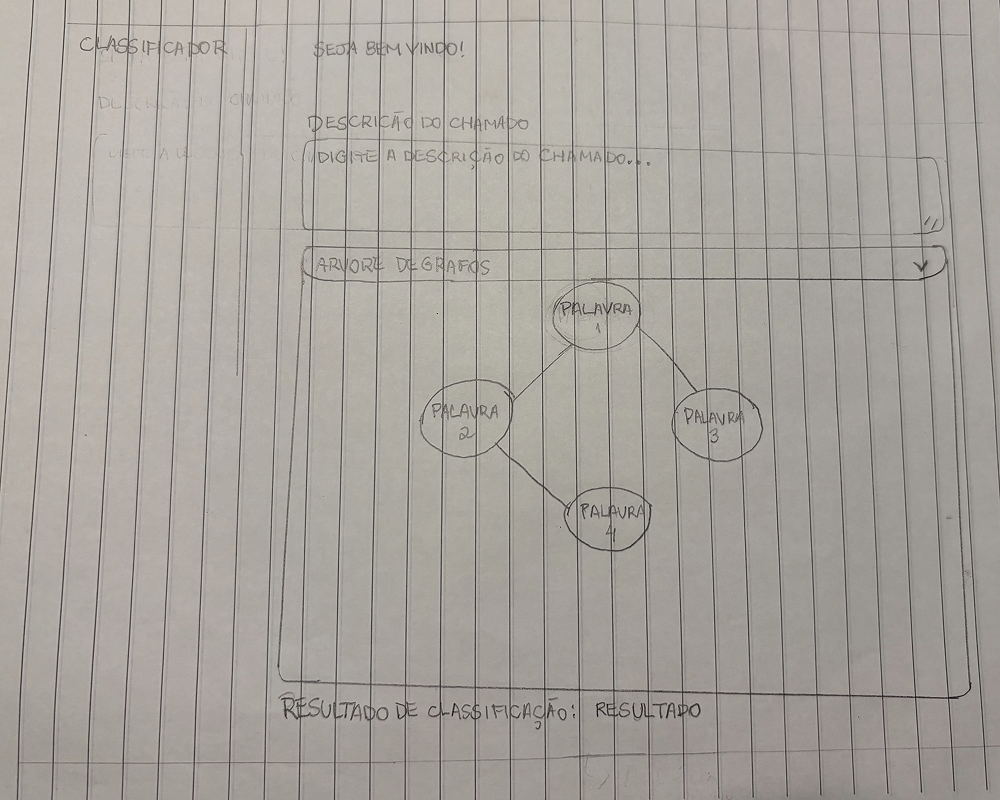
\includegraphics[width=0.75\textwidth]{imagens/baixa_agatha.png}
    \legend{Fonte: Elaborado pelos autores.}
\end{figure}

\begin{figure}[H]
    \caption{Protótipo de baixa fidelidade da interface (proposta 2)}
    \label{fig:prototipo_baixa_bru}
    \centering
    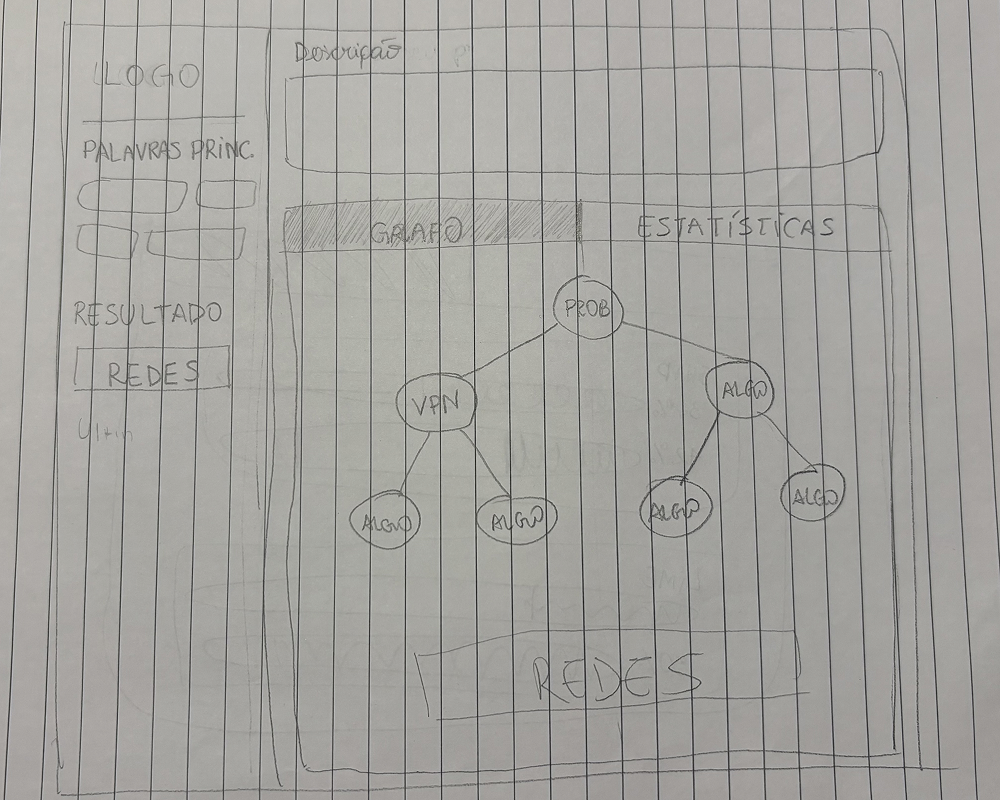
\includegraphics[width=0.75\textwidth]{imagens/baixa_bru.png}
    \legend{Fonte: Elaborado pelos autores.}
\end{figure}

\begin{figure}[H]
    \caption{Protótipo de baixa fidelidade da interface (proposta 3)}
    \label{fig:prototipo_baixa_kayke}
    \centering
    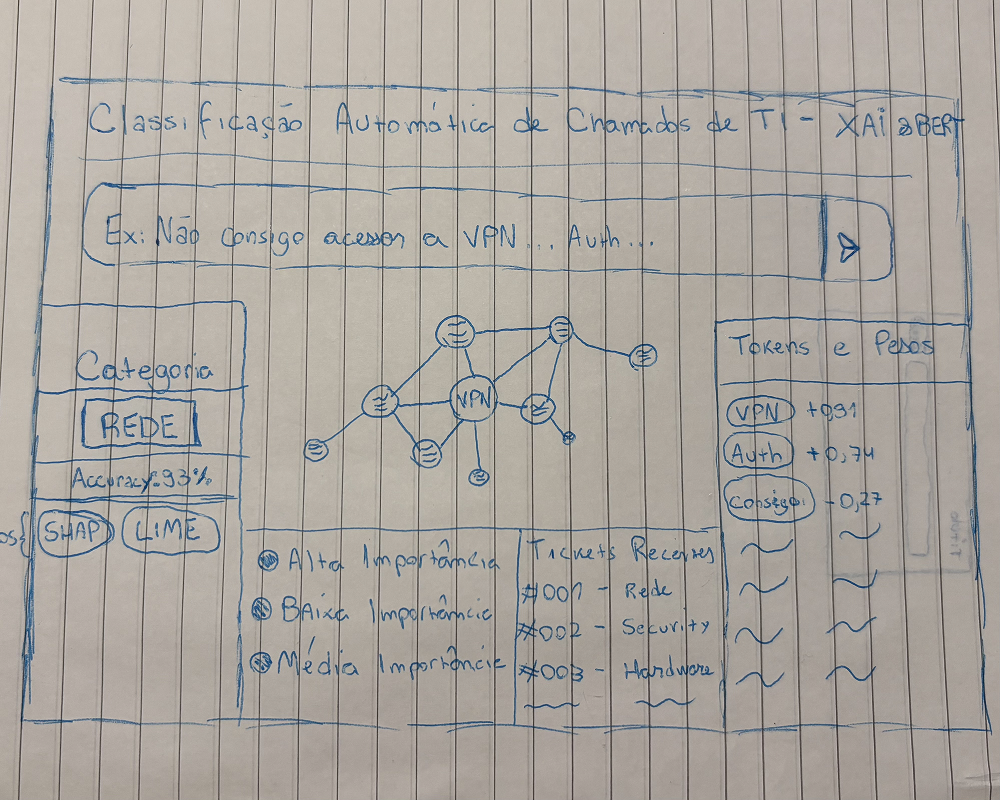
\includegraphics[width=0.75\textwidth]{imagens/baixa_kayke.png}
    \legend{Fonte: Elaborado pelos autores.}
\end{figure}

\begin{figure}[H]
    \caption{Protótipo de baixa fidelidade da interface final: tela do grafo}
    \label{fig:prototipo_baixa_grafo}
    \centering
    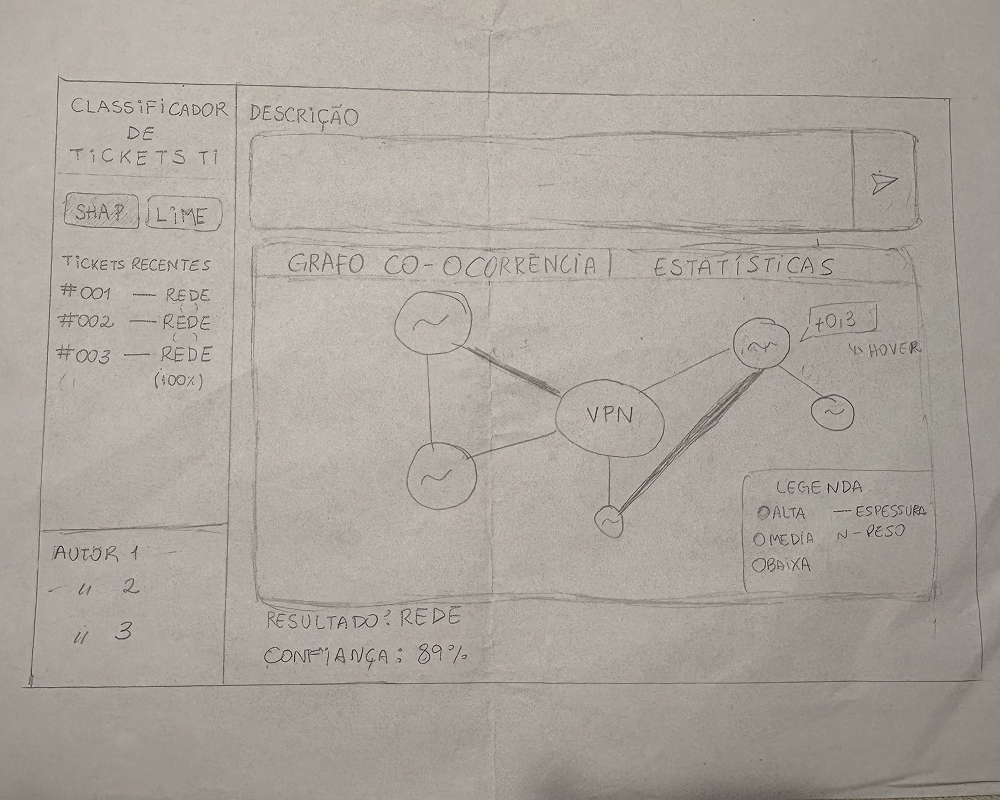
\includegraphics[width=0.75\textwidth]{imagens/baixa_grafo.png}
    \legend{Fonte: Elaborado pelos autores.}
\end{figure}

\begin{figure}[H]
    \caption{Protótipo de baixa fidelidade da interface final: tela das estatísticas}
    \label{fig:prototipo_baixa_estatisticas}
    \centering
    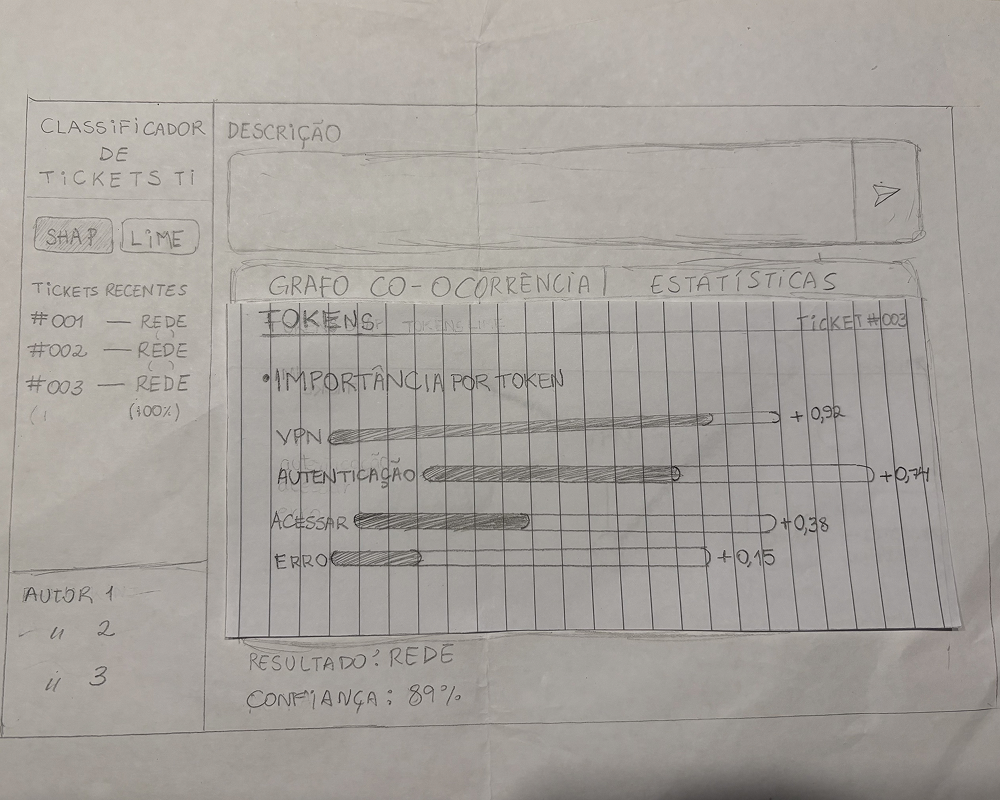
\includegraphics[width=0.75\textwidth]{imagens/baixa_estatisticas.png}
    \legend{Fonte: Elaborado pelos autores.}
\end{figure}

Posteriormente, foram elaborados protótipos de média fidelidade com maior nível de detalhamento visual, com foco em definir como as explicações geradas pelo modelo seriam apresentadas de forma compreensível para os analistas de TI. 

A área central do sistema é dedicada às explicações da 
classificação, organizada em duas abas principais, ambas voltadas 
para tornar o processo decisório do modelo auditável:

\begin{itemize}
    \item \textbf{Grafo de co-ocorrência}: representação visual das 
    relações entre as palavras do chamado, onde o tamanho de 
cada nó é proporcional à importância do termo (módulo do valor SHAP ou 
LIME, conforme o método escolhido em um seletor da interface), e a 
espessura de cada conexão cresce com o peso da aresta, dividido pelo maior peso do chamado;
    
    \item \textbf{Estatísticas}: painel que apresenta numericamente 
    a importância individual de cada palavra calculada pelos 
    métodos SHAP e LIME, permitindo ao analista comparar e validar 
    as contribuições de cada termo na decisão do modelo.
\end{itemize}

A escolha por disponibilizar tanto visualizações gráficas quanto 
estatísticas numéricas busca garantir que analistas com diferentes 
perfis consigam auditar as decisões do modelo, seja por meio de 
padrões visuais no grafo ou por comparações quantitativas entre os 
valores de importância das palavras.

Na lateral esquerda do sistema encontra-se a seção ``Tickets 
recentes'', responsável por apresentar classificações realizadas 
anteriormente juntamente com seus respectivos níveis de confiança. 
Esse recurso permite consultar rapidamente chamados processados 
anteriormente e auxilia na análise das classificações realizadas.

Os protótipos desenvolvidos tiveram como principal objetivo orientar a disposição dos recursos de explicabilidade na interface; esses protótipos não foram avaliados com analistas.

\begin{figure}[H]
    \caption{Protótipo de média fidelidade: visualização do grafo de co-ocorrência}
    \label{fig:prototipo_media_grafo}
    \centering
    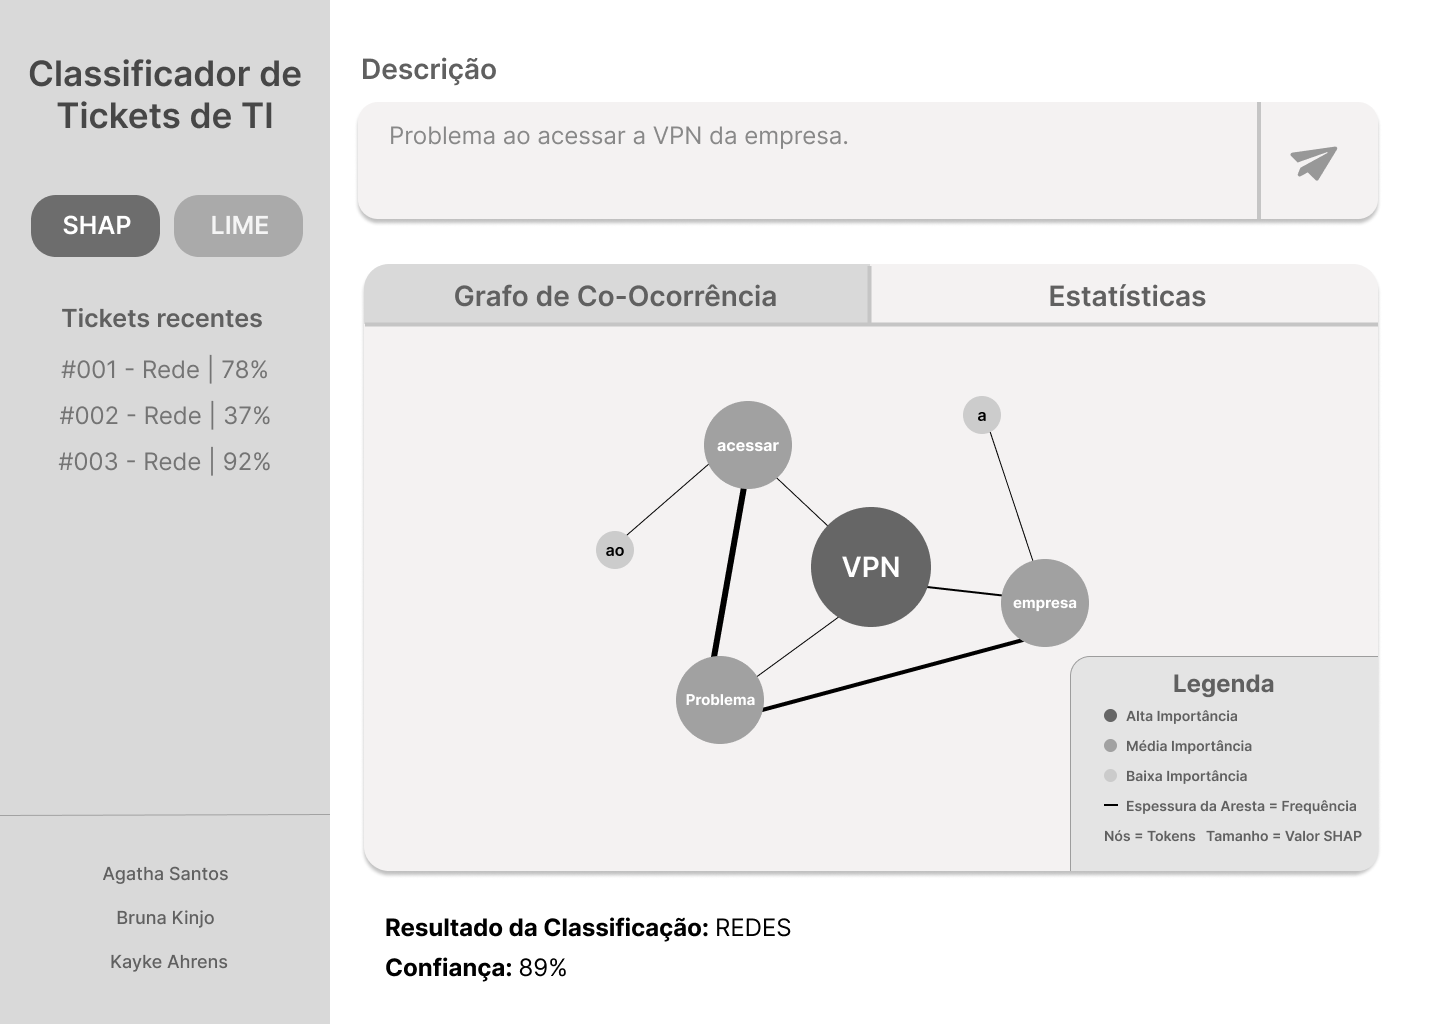
\includegraphics[width=0.75\textwidth]{imagens/grafo.png}
    \legend{Fonte: Elaborado pelos autores.}
\end{figure}

\begin{figure}[H]
    \caption{Protótipo de média fidelidade: visualização estatística das palavras}
    \label{fig:prototipo_media_estatisticas}
    \centering
    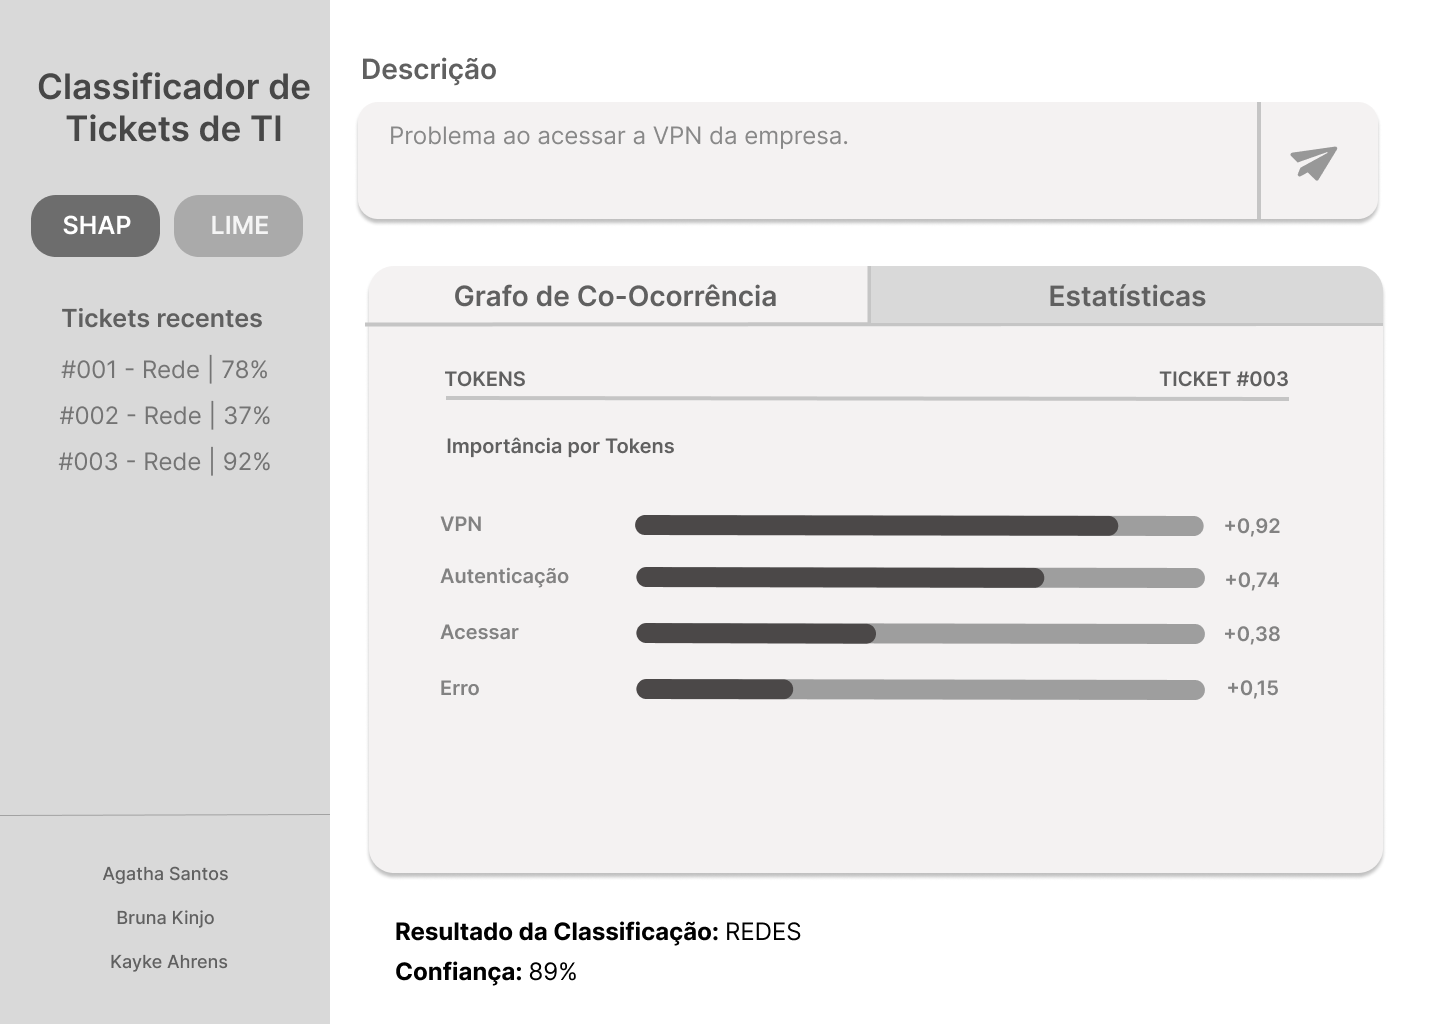
\includegraphics[width=0.75\textwidth]{imagens/estatisticas.png}
    \legend{Fonte: Elaborado pelos autores.}
\end{figure}

A Figura~\ref{fig:interface_final} mostra a interface final com um chamado inventado, digitado apenas para ilustração: a interface exibe a categoria prevista e a confiança, e o grafo de co-ocorrência, com nós em azul (a favor da classe prevista) e laranja (contra), o seletor entre SHAP e LIME e a lista de chamados recentes. A intensidade de cada cor (alta, média ou baixa) é definida pelos tercis dos valores do próprio chamado, e os nós laranja têm borda tracejada.
\begin{figure}[H]
    \caption{Interface final: classificação de um chamado digitado e grafo de co-ocorrência}
    \label{fig:interface_final}
    \centering
    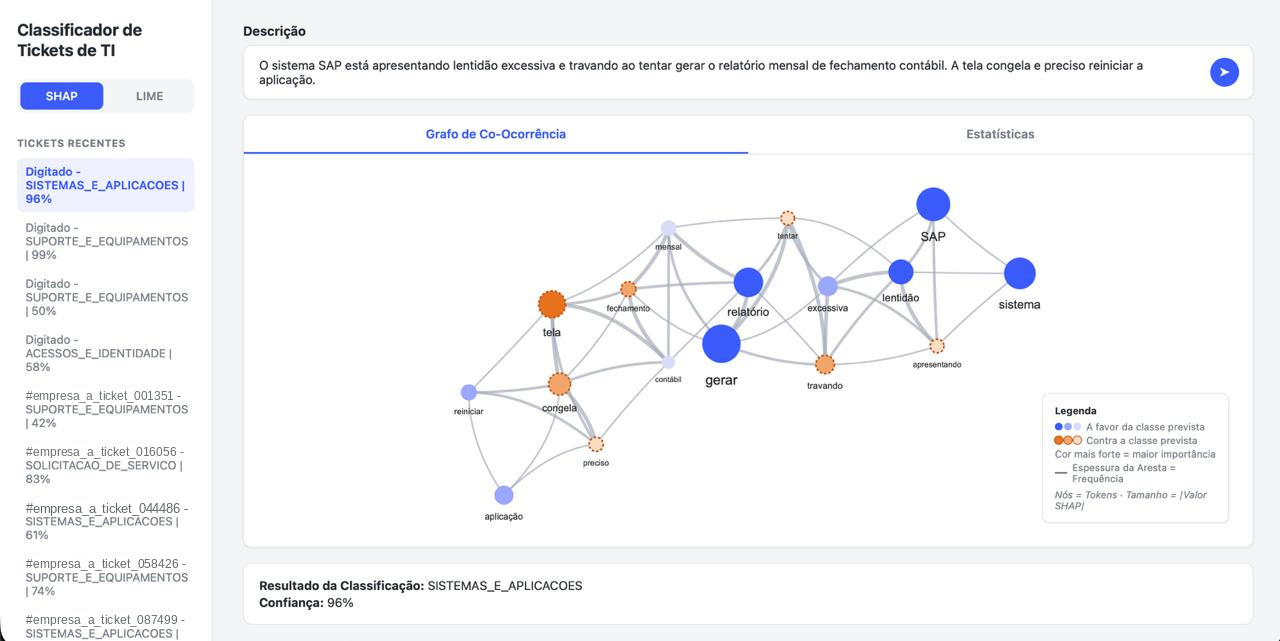
\includegraphics[width=\textwidth]{imagens/interface_final.jpg}
    \legend{Fonte: Elaborado pelos autores.\\ Nota: O chamado exibido é fictício, digitado apenas para ilustrar a interface, e não corresponde a nenhum chamado real das empresas ou dos dados do trabalho.}
\end{figure}

\subsubsection{Arquitetura da solução}

A arquitetura da solução é organizada em três camadas principais:

\begin{itemize}
    \item Camada de apresentação (\textit{front-end});
    \item Camada de processamento;
    \item Camada de dados.
\end{itemize}

A camada de apresentação é responsável pela interação com o usuário final, disponibilizando os formulários de inserção de chamados, exibição das classificações, visualização dos grafos e acesso ao histórico de chamados processados.

A camada de processamento é responsável pela execução das etapas de pré-processamento textual, inferência do modelo BERTimbau, cálculo das explicações utilizando SHAP e LIME, além da construção dos grafos de co-ocorrência.

Já a camada de dados é responsável pelo armazenamento das informações relacionadas aos chamados classificados e aos resultados gerados pelo sistema.

A Figura~\ref{fig:arquitetura} apresenta o diagrama de componentes da solução, com as três camadas e as interfaces entre elas.

\begin{figure}[H]
    \caption{Arquitetura da solução: diagrama de componentes UML}
    \label{fig:arquitetura}
    \centering
    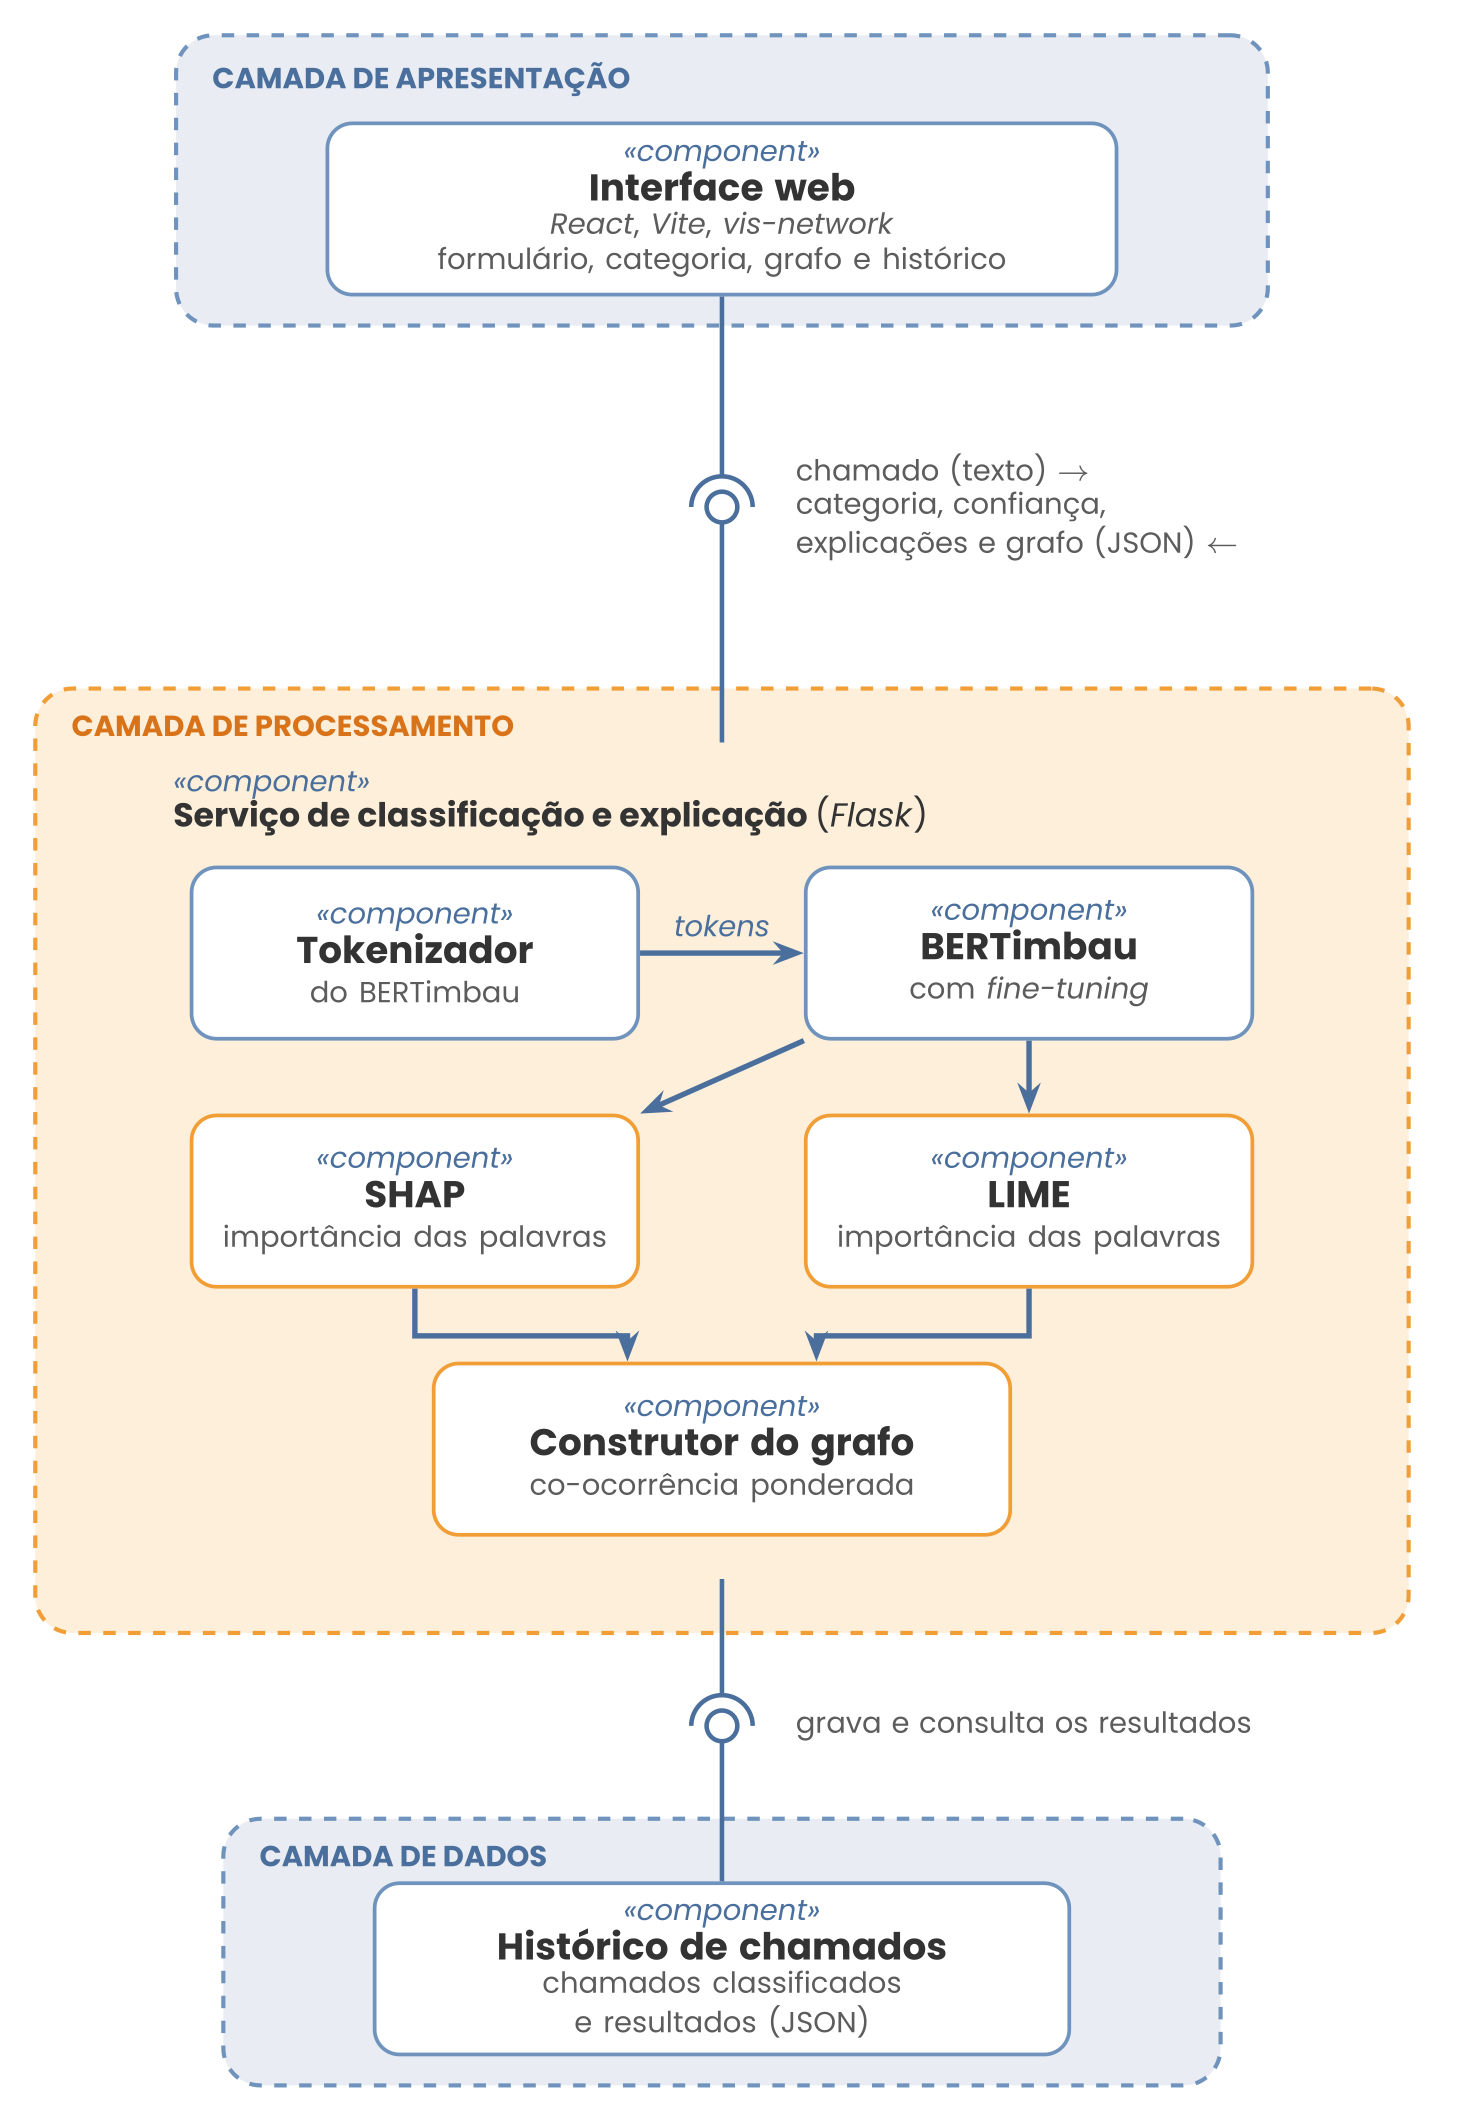
\includegraphics[width=0.82\textwidth]{imagens/uml_componentes.png}
    \legend{Fonte: Elaborado pelos autores.}
\end{figure}

O fluxo geral de funcionamento da aplicação segue as seguintes etapas:

\begin{enumerate}
    \item \textbf{Entrada do modelo}: a descrição curta e a descrição completa do chamado, sem remoção de \textit{stopwords}, são passadas como um par de textos ao tokenizador do BERTimbau, que as converte em \textit{tokens} com seus respectivos IDs e máscaras de atenção. A remoção de \textit{stopwords} é usada apenas na construção do grafo.

    \item \textbf{Classificação com BERTimbau}: o modelo BERTimbau com \textit{fine-tuning} processa a sequência de \textit{tokens} e produz, a partir da representação do \textit{token} [CLS], as probabilidades de pertencimento a cada categoria. A categoria com maior probabilidade é selecionada como predição, e o índice de confiança corresponde a essa probabilidade máxima. Essa confiança é a probabilidade máxima da \textit{softmax} e não foi calibrada, ou seja, uma confiança de 0,8 não significa necessariamente 80\% de acerto.

    \item \textbf{Cálculo de explicabilidade}: sobre o mesmo texto de entrada, são calculados os valores SHAP e as importâncias LIME. Cada palavra recebe um valor numérico que representa sua contribuição para a predição: valores positivos indicam contribuição para a classe predita, e valores negativos indicam contribuição contrária.

    \item \textbf{Construção do grafo de co-ocorrência}: as palavras do chamado são representadas como nós de um grafo $G = (V, E, W, f_{\text{shap}}, f_{\text{lime}})$. As arestas conectam pares de palavras que co-ocorrem dentro de uma janela deslizante de tamanho $w = 4$, com peso igual ao número de janelas que contêm o par. Os pesos dos \textbf{nós} são determinados pelos valores SHAP e LIME calculados na etapa anterior; as palavras com maior importância, segundo o método selecionado (SHAP ou LIME), geram nós visualmente maiores na interface. O grafo é serializado em JSON (\textit{JavaScript Object Notation} -- Notação de Objetos JavaScript), com os campos \texttt{tokens} (nós) e \texttt{arestas}, e enviado ao \textit{frontend}.

    \item \textbf{Apresentação ao analista}: a interface recebe o JSON, renderiza o grafo e exibe a categoria predita, o índice de confiança, as palavras destacadas por cor (azul, a favor da classe prevista; laranja, contra) e os valores SHAP e LIME comparativos.
\end{enumerate}


\subsection{Tecnologias e ferramentas}

As tecnologias estão na Tabela~\ref{tab:ferramentas}; a interface usa \textit{React}, \textit{Vite}, \textit{vis-network} e CSS (\textit{Cascading Style Sheets} -- Folhas de Estilo em Cascata), e a comunicação com o modelo usa \textit{Flask}.

\textbf{Ambiente de desenvolvimento:}

\begin{itemize}
    \item Git e GitHub;
    \item Máquinas locais dos integrantes do grupo.
\end{itemize}

\subsection{Funcionalidades principais}

Entre as principais funcionalidades implementadas no sistema estão:

\begin{itemize}
    \item \textbf{Funcionalidades de explicabilidade:}
    \begin{itemize}
        \item Construção de grafos de co-ocorrência;
        \item Visualização das explicações do modelo;
        \item Seleção do método de explicação (SHAP ou LIME) exibido no grafo.
    \end{itemize}
    \item \textbf{Funcionalidades de classificação e suporte:}
    \begin{itemize}
        \item Entrada do chamado em um único campo de texto;
        \item Classificação automática de chamados de TI;
        \item Exibição da categoria prevista;
        \item Apresentação do nível de confiança da classificação;
        \item Histórico simplificado de chamados classificados.
    \end{itemize}
\end{itemize}

\subsection{Metodologia de implementação}

A implementação do projeto seguiu uma abordagem iterativa, baseada em 
prototipação e validações incrementais.

Inicialmente foram realizados o levantamento bibliográfico, a 
definição dos requisitos e a elaboração dos protótipos da interface. 
Em seguida, foram preparados os dados, treinados os classificadores 
dos cenários A e B e implementados os módulos de explicabilidade 
(SHAP e LIME) e de construção do grafo de co-ocorrência. Por fim, 
esses módulos foram integrados à interface, que passou a gerar a 
explicação de um chamado digitado pelo \textit{pipeline} completo.

\subsection{Coleta e tratamento de dados}
\subsubsection{Origem e autorização de uso dos dados}
\label{subsubsec:autorizacao_dados}

Os dados utilizados neste trabalho são chamados reais de suporte
técnico cedidos por duas empresas do setor farmacêutico: Empresa B e Empresa A. Os autores solicitaram o
acesso por e-mail, explicando o objetivo acadêmico do trabalho, quais
informações seriam necessárias e como os registros seriam tratados.

Não foi utilizado um conjunto de dados público. Os chamados são dados privados das duas empresas, cedidos com finalidade acadêmica e anonimizados, e por isso os textos originais não são divulgados neste trabalho.

As autorizações de uso foram concedidas pelas duas empresas por e-mail.
Os autores se comprometeram a usar os chamados apenas neste trabalho e a
anonimizá-los antes de qualquer etapa de processamento. Essas mensagens
são o registro da autorização concedida e da finalidade acadêmica do uso, e estão
reproduzidas nos Anexos~\ref{an:autorizacao_empresa_a}
e~\ref{an:autorizacao_empresa_b}.

A anonimização, além de cumprir esse compromisso, alinha o trabalho ao
tratamento que a Lei Geral de Proteção de Dados Pessoais (LGPD, Lei
n.º 13.709/2018) dá aos dados anonimizados, que não são considerados
dados pessoais para os fins da lei, salvo quando a anonimização puder
ser revertida com esforços razoáveis \cite{brasil2018}. A etapa
descrita na Seção~\ref{subsubsec:dataset_finetuning} deixa de ser,
portanto, apenas uma escolha metodológica.



\subsubsection{\textit{Dataset} e \textit{fine-tuning}}
\label{subsubsec:dataset_finetuning}

A escolha do BERTimbau, e não do mBERT (\textit{BERT} multilíngue), deve-se a dois motivos. Primeiro, os chamados analisados estão em português brasileiro, pois a base foi filtrada por idioma (como descrito a seguir), e o BERTimbau possui representações mais ricas para esse idioma; na Tabela~\ref{tab:bertimbau_sota}, ele superou o mBERT nas quatro medidas. Segundo, os chamados utilizam terminologia técnica de TI em português, que pode diferir substancialmente da versão em inglês, e o BERTimbau, pré-treinado em corpus nacional, tem maior probabilidade de ter encontrado esse vocabulário durante o pré-treinamento.

O modelo BERTimbau, em sua versão \textit{base}, foi ajustado com chamados reais da Empresa A e da Empresa B, obtidos mediante autorização concedida por e-mail e anonimização dos registros. O arquivo da Empresa A tinha 191.350 chamados, abertos de maio de 2020 a agosto de 2026; após a remoção de duplicatas pelo número do chamado, o descarte de chamados sem categoria ou de categorias com menos de 100 chamados e a anonimização, restaram 189.909, dos quais 46.584 estavam em português e foram mantidos por um filtro de idioma. O arquivo da Empresa B tinha 9.317 chamados, todos de abril de 2026; após o descarte das categorias com menos de 100 chamados (restaram 8.758), dos chamados sem descrição (715) e de 326 cópias de uma mensagem automática de abertura por e-mail, todas da categoria de cibersegurança, restaram 7.717. As categorias das duas empresas foram harmonizadas em uma taxonomia única (Apêndice~\ref{ap:correspondencia_categorias}), e o conjunto combinado, com 54.301 chamados, passou ainda pelo descarte da classe com menos de 100 chamados (Recursos Humanos, 39 chamados) e pela remoção de 983 chamados, em 75 grupos de textos idênticos com categorias divergentes. Os resultados foram 53.279 chamados (Empresa B: 6.949; Empresa A: 46.330), em 11 classes, entre elas a classe OUTROS.

Na base da Empresa A, a anonimização foi feita antes de qualquer outro processamento, em duas camadas aplicadas à descrição curta e à descrição completa. A primeira, por expressões regulares, substituiu por marcadores os endereços de \textit{e-mail}, os endereços web, os números de chamado, os caminhos de arquivo, os endereços IP, os CPFs, os telefones, os identificadores de usuário e os nomes das empresas. A segunda usou o reconhecimento de entidades nomeadas do modelo \textit{pt\_core\_news\_md}, da biblioteca \textit{spaCy}, para substituir nomes de pessoas, de organizações e de locais, com uma lista de exceções para nomes de produtos e sistemas que fazem parte do vocabulário técnico, como SAP, Outlook e VPN. O número original de cada chamado foi descartado e trocado por um identificador sequencial.

Na base da Empresa B, a anonimização foi feita em duas etapas. Primeiro, um \textit{script} tratou os registros que seguiam uma estrutura regular. Os dados que o \textit{script} não alcançou foram revisados manualmente, e as informações sensíveis encontradas foram substituídas pelas mesmas máscaras já definidas para a anonimização automática.

Na base final usada no treino, a varredura de sanidade da anonimização encontrou 24 ocorrências residuais de padrão telefônico rotulado na descrição completa (0 no resumo), que podem incluir falsos positivos, como números de patrimônio depois de ``Tel:''.

As 11 classes da taxonomia harmonizada estão na Tabela~\ref{tab:categorias}.

\begin{table}[htb]
  \centering
  \caption{Categorias de classificação dos chamados}
  \label{tab:categorias}
  \footnotesize
  \setlength{\tabcolsep}{4pt}
  \begin{tabular}{p{5.5cm}p{6.2cm}r}
    \toprule
    Categoria & Tipo de chamado (exemplo) & Chamados no teste \\
    \midrule
    SISTEMAS\_E\_APLICACOES & Falhas e dúvidas em sistemas corporativos e aplicações & 2.458 \\
    ACESSOS\_E\_IDENTIDADE & Criação, bloqueio e revogação de acessos e contas (ex.: desligamento de colaborador) & 610 \\
    SUPORTE\_E\_EQUIPAMENTOS & Suporte a computadores e equipamentos (ex.: \textit{checklist} preventivo de salas de reunião) & 589 \\
    CONSULTA\_E\_ORIENTACAO & Dúvidas e pedidos de orientação & 555 \\
    REDES\_E\_COMUNICACOES & Rede, conectividade e comunicação & 435 \\
    SOFTWARE & Instalação e problemas de \textit{software} & 297 \\
    SOLICITACAO\_DE\_SERVICO & Pedidos de serviço (ex.: limpeza de um \textit{rack}) & 260 \\
    SERVIDORES & Chamados sobre servidores & 40 \\
    CIBERSEGURANCA & Segurança da informação & 21 \\
    AQUISICAO\_TI & Compra e licenciamento (ex.: transferência de licença do \textit{Office}) & 16 \\
    OUTROS & Categoria ``outros'' do sistema de aplicações da Empresa A (CORE\_OTHER) & 12 \\
    \bottomrule
  \end{tabular}
  \legend{Fonte: Elaborado pelos autores.}
\end{table}

A base da Empresa A possui, além da descrição completa, uma descrição curta, que a base da Empresa B não tem; nesse caso, o campo entra vazio. Ainda há chamados com texto repetido nas bases, sobretudo na Empresa B, o que motivou o agrupamento descrito a seguir.

O conjunto combinado foi dividido em 42.692 chamados de treino, 5.294 de validação e 5.293 de teste (proporção aproximada de 80/10/10). A divisão usou \textit{StratifiedGroupKFold} (8 partes para treino, 1 para validação e 1 para teste), estratificada pela categoria e agrupada pelo texto do chamado: chamados com texto idêntico ficam sempre na mesma parte.

O processo de \textit{fine-tuning} seguiu uma abordagem supervisionada de classificação textual. A entrada do modelo é o par formado pela descrição curta e pela descrição completa, limitado a 256 \textit{tokens}; cerca de 10,2\% dos pares ultrapassam esse limite. O treino usou 3 épocas, \textit{batch} de 16, taxa de aprendizado de $2 \times 10^{-5}$ e semente 42. Para reduzir o risco de \textit{overfitting}, fenômeno que ocorre quando o modelo aprende os dados de treino com precisão excessiva e perde a capacidade de generalizar para novos exemplos, o desempenho é acompanhado no conjunto de validação durante o treino. Não foram aplicadas técnicas de balanceamento de classes nem pesos por classe; o desbalanceamento é tratado na avaliação, com o uso do F1-macro. Uma tentativa posterior com pesos por classe, que não foi adotada, é descrita na Seção~\ref{subsec:res_melhoria}.


% ---------------------------------------------------------------
\section{Experimentos e cenários de teste}
\label{sec:experimentos}

Os experimentos seguiram os quatro cenários da Tabela~\ref{tab:cenarios}, todos sobre os mesmos conjuntos de treino, validação e teste descritos na Seção~\ref{subsubsec:dataset_finetuning}.

\subsection{Cenários A e B: classificação}

No cenário A, o \textit{baseline} SVM com TF-IDF foi treinado no conjunto de treino e avaliado no conjunto de teste, com a descrição curta e a descrição completa concatenadas como entrada. O TF-IDF usou unigramas e bigramas, frequência mínima de documento igual a 2 e escala sublinear; o classificador foi um \textit{LinearSVC} com $C = 1$, sem pesos de classe e semente 42. Assim como no BERTimbau, não foram removidas \textit{stopwords}.

O TF-IDF do \textit{scikit-learn} foi usado com frequência sublinear e \textit{idf} suavizado:

\begin{equation}
\mathrm{tf}'(t,d) = 1 + \ln \mathrm{tf}(t,d), \qquad
\mathrm{idf}(t) = \ln \frac{1 + N}{1 + \mathrm{df}(t)} + 1, \qquad
x_{t,d} = \frac{\mathrm{tf}'(t,d)\,\mathrm{idf}(t)}{\sqrt{\sum_{t'} \big(\mathrm{tf}'(t',d)\,\mathrm{idf}(t')\big)^2}}
\label{eq:tfidf-sklearn}
\end{equation}

O denominador normaliza cada vetor de chamado pela norma L2. Os termos são unigramas e bigramas que aparecem em pelo menos 2 chamados de treino.

O \textit{LinearSVC} treina um classificador por categoria (um contra todos). Para a categoria $c$, com $y_{ic} = +1$ se o chamado $i$ é da categoria $c$ e $-1$ caso contrário:

\begin{equation}
\min_{w_c,\, b_c} \; \frac{1}{2} \left( \lVert w_c \rVert^2 + b_c^2 \right)
+ C \sum_{i=1}^{N} \max\!\Big( 0,\; 1 - y_{ic}\,\big(w_c \cdot x_i + b_c\big) \Big)^2
\label{eq:svm}
\end{equation}

\begin{equation}
\hat{y} = \arg\max_{c} \; \big( w_c \cdot x + b_c \big)
\label{eq:svm-decisao}
\end{equation}

em que $x_i$ é o vetor TF-IDF do chamado (Equação~\ref{eq:tfidf-sklearn}), $C = 1$ controla o equilíbrio entre margem e erros, e a perda é a \textit{hinge} ao quadrado (padrão do \textit{LinearSVC}), com até 5.000 iterações.

No cenário B, o BERTimbau foi ajustado com a configuração da Seção~\ref{subsubsec:dataset_finetuning}. Os dois classificadores foram comparados pelas métricas da Seção~\ref{sec:metricas_avaliacao}, com destaque para o F1-macro.

\subsection{Cenário C: explicações SHAP e LIME}

As explicações foram geradas em 01/11/2026, para o modelo final, sobre uma amostra de 98 chamados do conjunto de teste: 8 acertos de cada uma das 10 classes que tiveram acertos (80 chamados) e 18 erros do modelo. A classe OUTROS não teve acertos, e por isso a amostra não tem 11 $\times$ 8 acertos. Foi necessário usar uma amostra porque SHAP e LIME explicam uma predição por vez, e explicar os 5.293 chamados do teste levaria cerca de 24 horas.

As explicações foram calculadas por palavra (sequência de letras e números, separada por espaços ou pontuação), e não por \textit{token} do BERTimbau; o termo \textit{token} é reservado à saída do tokenizador. No SHAP, cada palavra distinta do campo foi tratada como uma \textit{feature} (biblioteca \textit{shap}) e a probabilidade da classe predita foi o valor explicado. O LIME usou 500 amostras por explicação, largura do núcleo $\sigma = 25$ (padrão da biblioteca, não alterado) e peso para todas as palavras do campo, e não para um número fixo delas; a semente-base foi 42, derivada para cada chamado e campo. O campo explicado é perturbado e o outro campo fica com o texto original. O SHAP (versão 0.54.1) foi calculado de forma exata nos campos de até 10 palavras (87 campos); acima disso, foi estimado por amostragem, com orçamento de 2.000 consultas ao modelo (79 campos). No SHAP, as palavras ausentes foram apagadas do texto do campo explicado (e não trocadas por \texttt{[MASK]}), o outro campo foi mantido com o texto original, e o valor de referência é a probabilidade com o campo explicado sem nenhuma palavra. A fidelidade e a estabilidade seguiram a metodologia da Seção~\ref{subsec:criterios_validacao}; para a estabilidade, 12 chamados foram explicados 5 vezes cada. As cinco repetições de estabilidade usaram as sementes 42 a 46.

No conjunto de teste, a mediana é de 35 palavras por chamado (descrição curta e descrição completa juntas), a média é de 59,3 e 10\% dos chamados passam de 147 palavras. A descrição curta tem mediana de 5 palavras, mas 80\% das descrições completas têm mais de 10 palavras, ou seja, a maior parte dos chamados exigiria o SHAP por amostragem.

\subsection{Cenário D: grafo de co-ocorrência}
\label{subsec:cenario_d}

Para cada chamado explicado, construiu-se um grafo de co-ocorrência com janela deslizante de tamanho $w = 4$. As \textit{stopwords} foram removidas apenas nessa etapa, e não da entrada do modelo, porque o BERTimbau usa as palavras funcionais como contexto. As janelas ficam dentro de cada campo (descrição curta e descrição completa) e não passam de um campo para o outro, e palavras que diferem só pela caixa, como ``Impressora'' e ``impressora'', viram o mesmo nó. O peso de cada aresta é o número de janelas que contêm o par de palavras (frequência bruta, sem normalização), sem depender da distância entre elas dentro da janela; um par conta uma vez por janela, e cada janela gera no máximo $\binom{4}{2} = 6$ arestas (menos, se houver palavra repetida). O peso de cada nó é o módulo da soma dos pesos que o SHAP ou o LIME atribuiu à palavra (Equações~\ref{eq:aresta} e~\ref{eq:no}). O grafo foi avaliado por rastreabilidade, em casos aplicados (Seção~\ref{subsec:criterios_validacao}). O trabalho não implementou GCN: o grafo de co-ocorrência foi utilizado exclusivamente como estrutura de visualização das explicações, e não como componente do modelo de classificação.


% ---------------------------------------------------------------
\section{Resultados e análises}
\label{sec:resultados}

Esta seção apresenta os resultados dos cenários A a D, incluindo a tentativa de melhoria do classificador, e, em seguida, os analisa e os discute à luz da revisão bibliográfica e da hipótese de pesquisa.

\subsection{Desempenho da classificação (cenários A e B)}
\label{subsec:res_classificacao}

Para responder ao objetivo específico 1, a Tabela~\ref{tab:res_teste} apresenta o desempenho dos dois classificadores no conjunto de teste, com 5.293 chamados em 4.824 grupos de texto. O BERTimbau obteve F1-macro de 0,628 e o \textit{baseline} SVM com TF-IDF, de 0,591. A acurácia dos dois é próxima (0,724 e 0,719); a diferença aparece no F1-macro, que dá o mesmo peso a todas as classes, e vem da revocação (0,611 contra 0,550), pois a precisão é parecida (0,655 contra 0,662).

\begin{table}[htb]
  \centering
  \caption{Desempenho dos classificadores no conjunto de teste}
  \label{tab:res_teste}
  \small
  \setlength{\tabcolsep}{4pt}
  \begin{tabular}{lcccc}
    \toprule
    Modelo & Acurácia & Precisão (macro) & Revocação (macro) & F1-macro \\
    \midrule
    Cenário A: SVM + TF-IDF & 0,719 & 0,662 & 0,550 & 0,591 \\
    Cenário B: BERTimbau & 0,724 & 0,655 & 0,611 & 0,628 \\
    \bottomrule
  \end{tabular}
  \legend{Fonte: Elaborado pelos autores.}
\end{table}

A diferença de F1-macro a favor do BERTimbau foi de 3,7 pontos percentuais, com intervalo de confiança de 95\% de 1,0 a 6,7 (\textit{bootstrap} pareado por grupo de texto, 2.000 reamostragens). A diferença foi positiva em 99,8\% das reamostragens, mas a estimativa pontual fica abaixo da meta de 5 pontos estabelecida inicialmente (Seção~\ref{subsec:criterios_validacao}). Como o intervalo inclui os 5 pontos, os dados também não permitem descartar que a diferença verdadeira os alcance: em cerca de 21\% das reamostragens, a diferença atingiu ao menos 5 pontos.

A Tabela~\ref{tab:res_classe} mostra o F1 por classe. O ganho do BERTimbau se concentra em quatro classes: SOFTWARE e SOLICITACAO\_DE\_SERVICO, com diferenças de 8,5 e 8,0 pontos e intervalos que não incluem o zero, e SERVIDORES e AQUISICAO\_TI, classes pequenas (40 e 16 chamados) com intervalos largos. Juntas, essas quatro classes respondem por cerca de 96\% da diferença de 3,7 pontos no F1-macro. Na maior classe, SISTEMAS\_E\_APLICACOES (46\% do teste), os dois modelos praticamente empatam (0,811 e 0,809). Nenhum dos dois acertou chamados da classe OUTROS, que tem apenas 12 chamados no teste. Como o F1-macro dá o mesmo peso a todas as classes, o F1 nulo nessa classe reduz a média.

\begin{table}[htb]
  \centering
  \caption{F1 por classe no conjunto de teste e diferença entre BERTimbau e SVM}
  \label{tab:res_classe}
  \footnotesize
  \setlength{\tabcolsep}{3pt}
  \begin{tabular}{lrcccc}
    \toprule
    Classe & Chamados & F1 BERTimbau & F1 SVM & Dif. (p.p.) & IC 95\% (p.p.) \\
    \midrule
SISTEMAS\_E\_APLICACOES & 2.458 & 0,811 & 0,809 & +0,3 & $-$0,8 a 1,3 \\
ACESSOS\_E\_IDENTIDADE & 610 & 0,802 & 0,775 & +2,7 & 0,5 a 8,8 \\
SUPORTE\_E\_EQUIPAMENTOS & 589 & 0,722 & 0,731 & $-$0,8 & $-$3,8 a 1,8 \\
CONSULTA\_E\_ORIENTACAO & 555 & 0,429 & 0,429 & 0,0 & $-$4,3 a 3,9 \\
REDES\_E\_COMUNICACOES & 435 & 0,726 & 0,709 & +1,7 & $-$1,3 a 5,1 \\
SOFTWARE & 297 & 0,568 & 0,483 & +8,5 & 3,2 a 13,7 \\
SOLICITACAO\_DE\_SERVICO & 260 & 0,440 & 0,360 & +8,0 & 1,8 a 14,1 \\
SERVIDORES & 40 & 0,667 & 0,613 & +5,4 & $-$4,9 a 17,3 \\
CIBERSEGURANCA & 21 & 0,900 & 0,923 & $-$2,3 & $-$8,8 a 0,0 \\
AQUISICAO\_TI & 16 & 0,839 & 0,667 & +17,2 & $-$7,0 a 44,8 \\
OUTROS & 12 & 0,000 & 0,000 & 0,0 & 0,0 a 0,0 \\
    \bottomrule
  \end{tabular}
  \legend{Fonte: Elaborado pelos autores.\\ Nota: IC: intervalo de confiança por \textit{bootstrap} pareado; p.p.: pontos percentuais.}
\end{table}

A Tabela~\ref{tab:res_empresa} separa o teste por empresa. O F1-macro de cada empresa é calculado sobre as classes presentes em seus chamados (7 na Empresa B e 9 na Empresa A). Os dois modelos têm desempenho muito maior na Empresa B, e a diferença a favor do BERTimbau é de 1,3 ponto na Empresa B, com intervalo que inclui o zero, e de 4,0 pontos na Empresa A. Como a Empresa A reúne 86\% dos chamados de teste, o resultado geral reflete sobretudo essa empresa. Os 716 chamados da Empresa B formam apenas 337 grupos de texto, e um desses textos, um roteiro de desligamento de colaborador, aparece em 298 chamados da classe ACESSOS\_E\_IDENTIDADE, todos classificados corretamente pelos dois modelos. 
Sem esse grupo, restam 418 chamados da Empresa B, ainda nas mesmas 7 classes, e o F1-macro da empresa fica em 0,9014 (BERTimbau) e 0,8885 (SVM). A diferença continua de 1,3 ponto, o que mostra que esse grupo repetido não explica o resultado da Empresa B nem a diferença entre os modelos.

Parte da diferença entre as empresas pode vir da própria taxonomia: AQUISICAO\_TI e CIBERSEGURANCA só existem na Empresa B, e CONSULTA\_E\_ORIENTACAO, SOFTWARE, SOLICITACAO\_DE\_SERVICO e OUTROS só existem na Empresa A; apenas cinco classes são comuns às duas empresas. Assim, os chamados da Empresa B pertencem a apenas 7 das 11 classes, duas delas exclusivas da empresa.

\begin{table}[htb]
  \centering
  \caption{Desempenho no conjunto de teste, por empresa de origem}
  \label{tab:res_empresa}
  \footnotesize
  \setlength{\tabcolsep}{4pt}
  \begin{tabular}{lrrcccc}
    \toprule
    Subconjunto & Chamados & Grupos & F1 BERTimbau & F1 SVM & Dif. (p.p.) & IC de 95\% (p.p.) \\
    \midrule
    Empresa B & 716 & 337 & 0,911 & 0,897 & +1,3 & $-$3,1 a 5,9 \\
    Empresa A & 4.577 & 4.487 & 0,515 & 0,474 & +4,0 & 1,6 a 6,5 \\
    Total & 5.293 & 4.824 & 0,628 & 0,591 & +3,7 & 1,0 a 6,7 \\
    \bottomrule
  \end{tabular}
  \legend{Fonte: Elaborado pelos autores.\\ Nota: Grupos: conjuntos de chamados com texto idêntico.}
\end{table}

No conjunto de validação, a diferença segue a mesma direção. Após retirar um bloco de 491 chamados de SUPORTE\_E\_EQUIPAMENTOS com o mesmo texto (um \textit{checklist} preventivo de salas de reunião, que o SVM classificou como REDES\_E\_COMUNICACOES e o BERTimbau como SUPORTE\_E\_EQUIPAMENTOS), restam 4.803 chamados, nos quais o F1-macro foi de 0,591 para o BERTimbau e 0,555 para o SVM, uma diferença de 3,5 pontos (intervalo de 95\% de 1,3 a 6,1). Na validação inteira, de 5.294 chamados, a diferença seria de 11,9 pontos, inflada por esse único texto.

A Figura~\ref{fig:matriz_confusao} mostra a matriz de confusão do BERTimbau no teste, normalizada por classe real; as contagens citadas a seguir são absolutas. Os erros mais frequentes ocorrem entre CONSULTA\_E\_ORIENTACAO e SISTEMAS\_E\_APLICACOES (180 chamados previstos como a segunda e 146 no sentido inverso), seguidos de SOLICITACAO\_DE\_SERVICO previstos como SISTEMAS\_E\_APLICACOES (78) e de SISTEMAS\_E\_APLICACOES previstos como SUPORTE\_E\_EQUIPAMENTOS (76). As classes de menor F1 são CONSULTA\_E\_ORIENTACAO (0,429), SOLICITACAO\_DE\_SERVICO (0,440) e OUTROS (0,000). Uma possível explicação, que este trabalho não testou, é que essas classes descrevem o tipo de pedido, e não o sistema ou equipamento envolvido, e por isso se sobrepõem às demais.

\begin{figure}[H]
    \caption{Matriz de confusão do BERTimbau no conjunto de teste, normalizada por classe real}
    \label{fig:matriz_confusao}
    \centering
    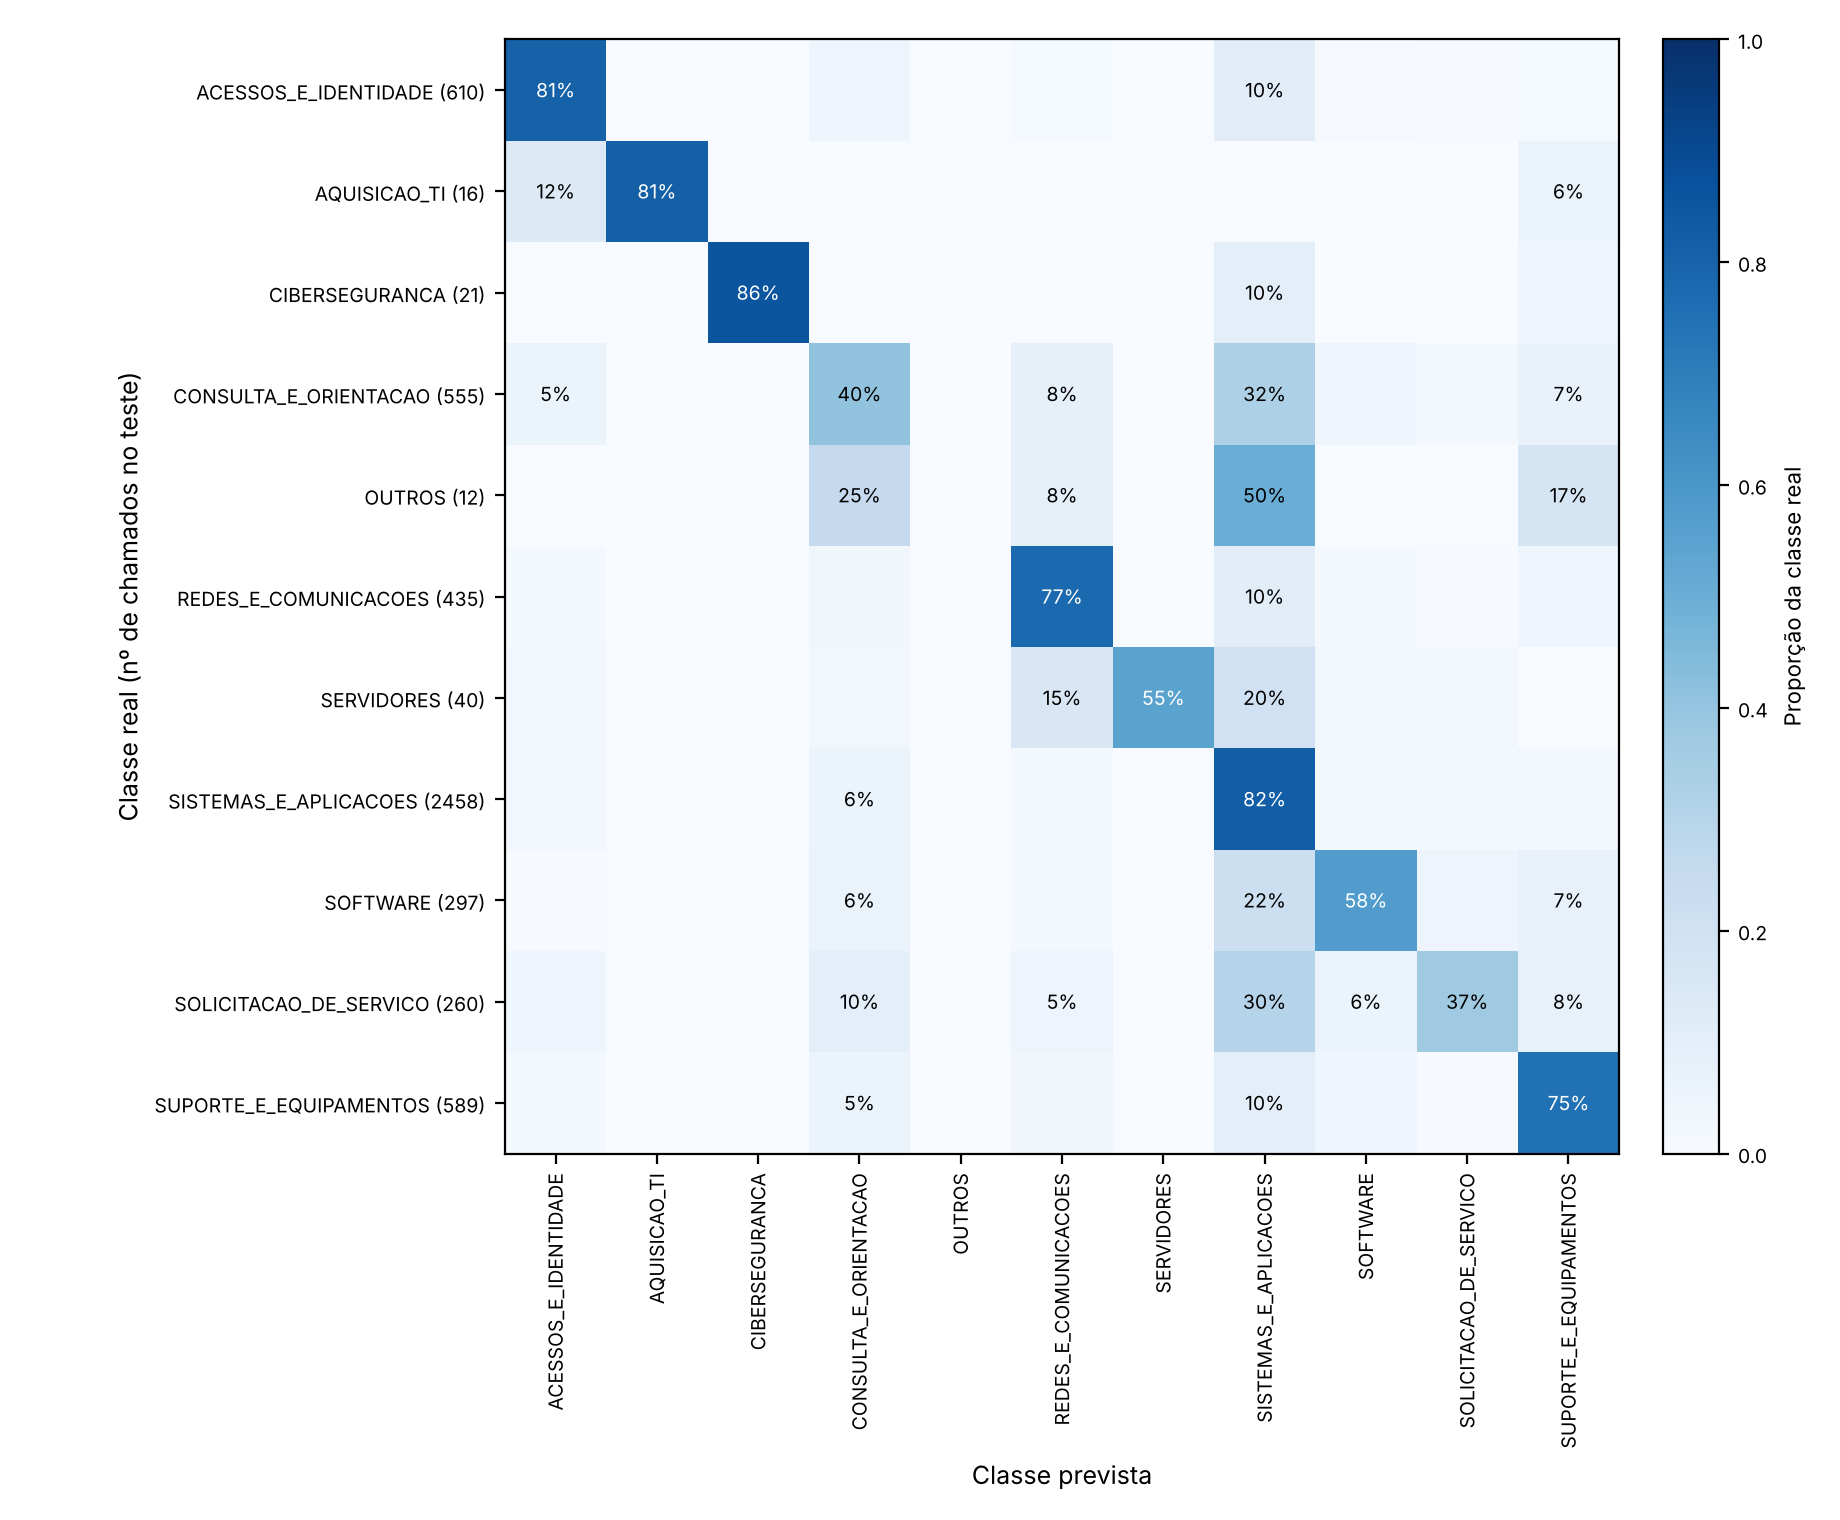
\includegraphics[width=0.9\textwidth]{imagens/matriz_confusao_teste.png}
    \legend{Fonte: Elaborado pelos autores.\\ Nota: Cada linha soma 100\% dos chamados da classe real; por isso a matriz não é simétrica, e as células acima e abaixo da diagonal mostram erros diferentes.}
\end{figure}

\subsection{Tentativa de melhoria do classificador (C1 e S1)}
\label{subsec:res_melhoria}

Depois do treino de referência, o grupo avaliou se pesos de classe na função de perda melhorariam o desempenho nas classes pequenas. Para que a escolha não fosse influenciada pelos resultados, o plano do experimento foi declarado em 21/10/2026, antes de qualquer execução, em um documento de experimentos declarados. O candidato C1 manteve toda a configuração do ajuste fino (Seção~\ref{subsubsec:dataset_finetuning}) e a mesma divisão dos dados, mudando apenas a perda: cada classe $c$ recebeu um peso proporcional a $1/\sqrt{n_c}$, normalizado para que o peso médio por exemplo de treino seja 1,

\begin{equation}
w_c = \frac{\tilde w_c}{\frac{1}{N}\sum_{i=1}^{N} \tilde w_{y_i}}, \qquad
\tilde w_c = \frac{1}{\sqrt{n_c}}
\label{eq:pesos-c1}
\end{equation}
em que $n_c$ é o número de chamados da classe $c$ no treino e $N$ é o total de chamados de treino. No treino, essa perda é calculada a cada lote $B$, no padrão do PyTorch quando a entropia cruzada recebe um peso por classe:

\begin{equation}
\mathcal{L}_B = -\frac{\sum_{i \in B} w_{y_i} \log p(y_i \mid x_i)}{\sum_{i \in B} w_{y_i}}
\label{eq:perda-c1}
\end{equation}

Como o denominador é a soma dos pesos do próprio lote, a normalização da Equação~\ref{eq:pesos-c1} fixa a escala dos pesos e não altera o valor da perda. % CONFERIDO: finetune_bertimbau.py usa cross_entropy com peso por classe; o PyTorch divide pela soma dos pesos do lote.

A seleção usaria apenas a validação corrigida, que retira o bloco de 491 chamados com o mesmo texto (Seção~\ref{subsec:res_classificacao}), sem abrir o conjunto de teste. O C1 seria aceito somente se três condições valessem ao mesmo tempo, sobre as sementes 42, 43 e 44:

\begin{enumerate}
  \item a média do F1-macro das três sementes ser ao menos 2 pontos maior que a do modelo de referência;
  \item cada semente, sozinha, ficar acima da referência;
  \item a diferença entre a média das três sementes e a referência ser positiva em ao menos 90\% das 2.000 reamostragens do \textit{bootstrap} pareado por grupo.
\end{enumerate}

Foi declarada também uma regra de parada: se uma semente ficasse igual ou abaixo da referência, a condição 2 já estaria descumprida, e as demais sementes seriam dispensadas. Para o SVM, foi declarada a variação S1, com pesos de classe balanceados (parâmetro \texttt{class\_weight} igual a \texttt{"balanced"}).

A Tabela~\ref{tab:res_melhoria} traz o resultado na validação corrigida (4.803 chamados em 4.536 grupos, 11 classes). Os valores têm quatro casas decimais para que as diferenças possam ser conferidas.

\begin{table}[htb]
  \centering
  \caption{Candidatos de melhoria na validação corrigida}
  \label{tab:res_melhoria}
  \footnotesize
  \setlength{\tabcolsep}{3pt}
  \begin{tabular}{>{\raggedright\arraybackslash}p{2.6cm}>{\raggedright\arraybackslash}p{2.4cm}ccccc}
    \toprule
    Candidato & Referência & F1 cand. & F1 ref. & Dif. (p.p.) & IC 95\% (p.p.) & Ganho $>0$ \\
    \midrule
    C1 (BERTimbau, semente 42) & BERTimbau de referência & 0,5772 & 0,5906 & $-$1,3 & $-$3,0 a $+$0,3 & 5\% \\
    S1 (SVM balanceado) & SVM original & 0,5577 & 0,5552 & $+$0,3 & $-$2,0 a $+$2,7 & 55\% \\
    \bottomrule
  \end{tabular}
  \legend{Fonte: Elaborado pelos autores.\\ Nota: F1: F1-macro; cand.: candidato; ref.: referência; IC: intervalo de confiança por \textit{bootstrap} pareado por grupo; p.p.: pontos percentuais; Ganho $>0$: fração das 2.000 reamostragens com diferença positiva.}
\end{table}

O C1 foi treinado com a semente 42 na GTX 1650 (8.007 passos de atualização), em execução iniciada em 21/10/2026. Na validação inteira, obteve F1-macro de 0,6197 (acurácia de 0,7106), contra 0,6303 da referência. Na validação corrigida, ficou 1,3 ponto abaixo da referência, e a diferença foi positiva em apenas 5\% das reamostragens; em relação ao SVM original, ficou 2,2 pontos acima (intervalo de 95\% de $-$0,5 a $+$4,9). A condição 2 falhou. Em 26/10/2026, quando o intervalo foi calculado, as sementes 43 e 44 foram dispensadas pela regra de parada, e o conjunto de teste não foi aberto para o C1.

O S1 foi executado em 21/10/2026 (cerca de 2 minutos, sem uso do teste). Obteve F1-macro de 0,5170 na validação inteira (acurácia de 0,6128) e de 0,5577 na validação corrigida, 0,3 ponto acima do SVM original, com intervalo que inclui o zero e diferença positiva em 55\% das reamostragens. Como o ganho não foi comprovado, o S1 não foi aprovado, e o SVM original continuou sendo a referência do cenário A.

Nenhum dos dois candidatos foi aprovado. Em 26/10/2026, o grupo decidiu manter como modelo final o BERTimbau treinado de 04/10 a 05/10/2026, usado em todos os resultados, nas explicações e na interface, e o modelo foi congelado em 28/10/2026.

A escolha do escopo combinado (Empresa A e Empresa B) para essa tentativa foi feita depois de observados os resultados de teste do modelo de referência e de um modelo treinado só com chamados da Empresa A; por isso, o resultado da tentativa é relatado como complementar. O modelo só com a Empresa A foi treinado com outra divisão dos dados, e apenas 468 chamados estão no teste dos dois, o que impede uma comparação pareada entre eles; essa comparação não foi feita.

\subsection{Explicabilidade: SHAP e LIME (cenário C)}
\label{subsec:res_xai}
Para responder ao objetivo específico 2, as explicações do SHAP e do LIME foram geradas para os 98 chamados da amostra (Seção~\ref{subsec:criterios_validacao}). Em CPU, em um computador Apple, o LIME levou 964 segundos (cerca de 16 minutos) e o SHAP, 3.039 segundos (cerca de 51 minutos). No SHAP, a soma dos pesos das palavras com a probabilidade-base reproduziu a probabilidade do chamado em todas as explicações, com erro máximo da ordem de $10^{-15}$. No LIME, o $R^2$ do modelo linear local, ponderado pela proximidade, teve mediana de 0,68, com mínimo de 0,11.

\subsubsection{Fidelidade}
\label{subsubsec:res_fidelidade}

A Tabela~\ref{tab:res_fidelidade} traz a fidelidade dos dois métodos nos 98 chamados. Na \textit{comprehensiveness}, mede-se a queda da probabilidade da classe prevista ao retirar as palavras apontadas pelo método (quanto maior, melhor); na \textit{sufficiency}, a queda ao manter apenas essas palavras (quanto menor, melhor); o Tau-LOO é a correlação de Kendall entre o peso de cada palavra e a queda de probabilidade ao retirá-la sozinha (quanto maior, melhor). As duas primeiras são comparadas à queda obtida com palavras sorteadas.

\begin{table}[htb]
  \centering
  \caption{Fidelidade das explicações do SHAP e do LIME nos 98 chamados da amostra}
  \label{tab:res_fidelidade}
  \small
  \begin{tabular}{p{4.6cm}lccc}
    \toprule
    Medida & Método & Explicação & Aleatório & Acima do acaso \\
    \midrule
    \textit{Comprehensiveness} (maior é melhor) & LIME & 0,542 & 0,192 & 94 de 98 \\
     & SHAP & 0,546 & 0,189 & 96 de 98 \\
    \addlinespace
    \textit{Sufficiency} (menor é melhor) & LIME & 0,019 & 0,309 & 96 de 98 \\
     & SHAP & 0,005 & 0,311 & 95 de 98 \\
    \addlinespace
    Tau-LOO (maior é melhor) & LIME & 0,412 & -- & 95 de 98 \\
     & SHAP & 0,361 & -- & 95 de 98 \\
    \bottomrule
  \end{tabular}
  \legend{Fonte: Elaborado pelos autores.\\ Nota: Valores médios por chamado. Cinco sorteios aleatórios por chamado, semente 42. ``Acima do acaso'': chamados em que a explicação supera o sorteio. No Tau-LOO não há linha de base aleatória, e a última coluna indica os chamados com valor positivo.}
\end{table}

Os dois métodos ficam bem acima do acaso nas três medidas. Retirar as palavras apontadas reduz a probabilidade da classe prevista em 0,54 (LIME) e 0,55 (SHAP), contra 0,19 nos dois ao retirar palavras sorteadas, e manter só as palavras apontadas deixa a probabilidade quase inalterada (queda de 0,019 e 0,005), contra 0,31 nos dois com palavras sorteadas. As diferenças entre os métodos são pequenas: o SHAP tem valores um pouco melhores na \textit{comprehensiveness} (0,546 contra 0,542) e na \textit{sufficiency} (0,005 contra 0,019), e o LIME, um Tau-LOO maior (0,412 contra 0,361).
Para comparar os métodos nos mesmos chamados, calculou-se a diferença SHAP menos LIME em cada chamado, com intervalo de confiança de 95\% por \textit{bootstrap} sobre os chamados (5.000 reamostragens, semente 42). Na \textit{comprehensiveness}, a diferença média foi de 0,004 (intervalo de $-0{,}020$ a 0,028), e na \textit{sufficiency}, de $-0{,}014$ (intervalo de $-0{,}037$ a 0,004); os dois intervalos incluem o zero, e os dados não distinguem os métodos nessas medidas. No Tau-LOO, a diferença foi de $-0{,}051$ (intervalo de $-0{,}081$ a $-0{,}020$), ou seja, o LIME teve correlação maior com o efeito de retirar cada palavra. % CONFERIDO: diferencas pareadas com fidelidade_shap_por_chamado.csv (SHAP, 2.000) e fidelidade_por_chamado.csv (LIME, 500); bootstrap de 5.000, semente 42.

\subsubsection{Estabilidade}
\label{subsubsec:res_estabilidade}

A estabilidade foi medida em 12 chamados com ao menos oito palavras distintas, explicados 5 vezes cada, com as sementes 42 a 46 (Tabela~\ref{tab:res_estabilidade}). Em 3 desses chamados, todos os campos têm até 10 palavras e o SHAP foi calculado de forma exata, sem sorteio, de modo que a explicação é idêntica nas cinco repetições (estabilidade 1 por construção). Nos outros 9, ao menos um campo foi estimado por amostragem, com orçamento de 2.000 consultas, e o SHAP variou de uma repetição para outra.

\begin{table}[htb]
  \centering
  \caption{Estabilidade das explicações do SHAP e do LIME em 12 chamados, com 5 repetições}
  \label{tab:res_estabilidade}
  \small
  \begin{tabular}{p{3.9cm}rccc}
    \toprule
    Método & Chamados & Jaccard (acaso) & Spearman & Topo igual (acaso) \\
    \midrule
    LIME & 12 & 0,659 (0,213) & 0,774 & 0,950 (0,062) \\
    SHAP, todos & 12 & 0,725 (0,213) & 0,896 & 0,875 (0,062) \\
    SHAP, só amostragem & 9 & 0,634 (0,135) & 0,861 & 0,833 (0,043) \\
    \bottomrule
  \end{tabular}
  \legend{Fonte: Elaborado pelos autores.\\ Nota: Valores médios por chamado. Jaccard: das 5 palavras mais relevantes entre as repetições. ``Topo igual'': fração dos pares de repetições com a mesma palavra no topo. Entre parênteses, o valor esperado ao acaso. ``Só amostragem'' exclui os 3 chamados em que o SHAP foi exato.}
\end{table}

Os dois métodos ficam acima do acaso nas três medidas, mas nenhum é perfeitamente estável. O LIME manteve a mesma palavra no topo em 95\% dos pares de repetições e teve Jaccard de 0,659. O SHAP teve Jaccard de 0,725 e a mesma palavra no topo em 88\% dos pares de repetições; considerando só os 9 chamados em que houve amostragem, os valores caem para 0,634 e 83\%. Nos 9 chamados em que houve amostragem, a comparação é direta, com os mesmos chamados nos dois métodos: o LIME teve Jaccard de 0,546 contra 0,634 do SHAP, Spearman de 0,706 contra 0,861 e a mesma palavra no topo em 93\% dos pares de repetições contra 83\%. Nessa amostra, portanto, o SHAP estimado por amostragem, com 2.000 consultas, foi mais estável que o LIME no Jaccard e no Spearman e menos estável na mesma palavra no topo; só o cálculo exato dá estabilidade total ao SHAP. Como cerca de 80\% das descrições completas do teste têm mais de 10 palavras, a maior parte dos chamados reais cairia no SHAP por amostragem, o que torna essa limitação relevante na prática. Como são apenas 12 chamados e não houve teste estatístico, o resultado é indicativo.

Para escolher o orçamento do SHAP, a estabilidade dos campos estimados por amostragem foi medida em 20 chamados com 500, 2.000 e 5.000 consultas por campo (Tabela~\ref{tab:res_orcamento}). A estabilidade aumentou com o orçamento nas três medidas. Adotou-se 2.000 consultas, que melhora bastante a estabilidade em relação a 500 com cerca de 2,5 vezes menos consultas ao modelo que 5.000. % CONFERIDO: estabilidade dos 12 chamados em orcamento_2000/estabilidade/estabilidade_shap_resumo.json (0,725; 0,896; 0,875 e, so amostragem, 0,634; 0,861; 0,833). Orcamentos de 20 chamados: 500 = 0,598; 0,684; 0,815; 2.000 = 0,719; 0,859; 0,925; 5.000 = 0,799; 0,920; 0,970.

\begin{table}[htb]
  \centering
  \caption{Estabilidade do SHAP estimado por amostragem em 20 chamados, por orçamento de consultas}
  \label{tab:res_orcamento}
  \small
  \begin{tabular}{rccc}
    \toprule
    Orçamento (consultas) & Jaccard (acaso) & Spearman & Topo igual (acaso) \\
    \midrule
    500 & 0,598 (0,131) & 0,684 & 0,815 (0,042) \\
    2.000 & 0,719 (0,131) & 0,859 & 0,925 (0,042) \\
    5.000 & 0,799 (0,131) & 0,920 & 0,970 (0,042) \\
    \bottomrule
  \end{tabular}
  \legend{Fonte: Elaborado pelos autores.\\ Nota: Valores médios por chamado, em 20 chamados com ao menos um campo estimado por amostragem, explicados 5 vezes cada. Jaccard: das 5 palavras mais relevantes entre as repetições. ``Topo igual'': fração dos pares de repetições com a mesma palavra no topo. Entre parênteses, o valor esperado ao acaso.}
\end{table}

\subsubsection{Concordância entre SHAP e LIME}
\label{subsubsec:res_concordancia}

A concordância compara, para cada um dos 98 chamados, as palavras que o SHAP e o LIME apontaram como importantes para a classe prevista. Como os pesos estão em escalas diferentes (probabilidade no SHAP, coeficiente do modelo linear local no LIME), a comparação usa a ordem e o sinal das palavras, e não o valor dos pesos. A palavra do topo e as cinco mais relevantes são as de maior peso em módulo. A Tabela~\ref{tab:res_concordancia} mostra o resultado, ao lado do valor esperado ao acaso.

\begin{table}[htb]
  \centering
  \caption{Concordância entre SHAP e LIME nos 98 chamados da amostra}
  \label{tab:res_concordancia}
  \small
  \begin{tabular}{p{5.6cm}ccc}
    \toprule
    Medida & Resultado & Ao acaso & Chamados acima do acaso \\
    \midrule
    Correlação de Spearman entre os pesos (média) & 0,735 & 0,000 & 98 de 98 \\
    Jaccard das 5 palavras mais relevantes (média) & 0,585 & 0,226 & 91 de 96 \\
    Mesma palavra no topo (fração de chamados) & 0,694 (68 de 98) & 0,068 & -- \\
    Palavras com o mesmo sinal (média) & 0,805 & 0,500 & 93 de 98 \\
    \bottomrule
  \end{tabular}
  \legend{Fonte: Elaborado pelos autores.\\ Nota: O Jaccard considera apenas os 96 chamados com mais de 5 palavras.}
\end{table}

Nas quatro medidas, os dois métodos concordam bem acima do acaso, mas longe da concordância total. Em 68 dos 98 chamados (69\%) os dois colocam a mesma palavra no topo, contra 7\% esperados ao acaso, e a mediana da correlação de Spearman é 0,803. A concordância não indica qual dos métodos está certo, apenas que apontam as mesmas palavras; a fidelidade de cada um é tratada à parte.

A Tabela~\ref{tab:res_concordancia_grupos} separa os chamados por forma de cálculo do SHAP e por acerto do modelo. A concordância é maior nos 27 chamados em que o SHAP foi calculado de forma exata (Spearman de 0,856) do que nos 71 em que houve amostragem (0,689). Os chamados do primeiro grupo são os mais curtos, então os dados não separam o efeito do método de cálculo do efeito do tamanho do texto. Em todos os chamados, a correlação entre o número de palavras e a concordância de Spearman é de $-0{,}60$ ($p < 0{,}001$): quanto mais palavras, menos os dois métodos concordam. Já entre acertos e erros do modelo, a concordância fica próxima (Spearman de 0,733 nos acertos e de 0,746 nos erros), com amostra de erros pequena (18 chamados). % CONFERIDO: concordancia_shap_lime.py escolhe topo e 5 palavras pelo maior peso em modulo; Spearman so nas palavras comuns, com sinal. Recalculado com shap_explicacoes.csv (2.000) e lime_explicacoes.csv (500): 68 de 98 no topo.

\begin{table}[htb]
  \centering
  \caption{Concordância entre SHAP e LIME por subconjunto de chamados}
  \label{tab:res_concordancia_grupos}
  \small
  \begin{tabular}{lrcccc}
    \toprule
    Subconjunto & Chamados & Spearman & Jaccard & Mesmo topo & Mesmo sinal \\
    \midrule
    Todos & 98 & 0,735 & 0,585 & 0,694 & 0,805 \\
    SHAP exato & 27 & 0,856 & 0,752 & 0,704 & 0,900 \\
    SHAP por amostragem & 71 & 0,689 & 0,526 & 0,690 & 0,769 \\
    Acertos do modelo & 80 & 0,733 & 0,593 & 0,688 & 0,802 \\
    Erros do modelo & 18 & 0,746 & 0,549 & 0,722 & 0,819 \\
    \bottomrule
  \end{tabular}
  \legend{Fonte: Elaborado pelos autores.\\ Nota: Valores médios por chamado; ``Mesmo topo'' é a fração de chamados com a mesma palavra no topo. O Jaccard considera apenas chamados com mais de 5 palavras (25 no SHAP exato, 71 na amostragem, 79 nos acertos e 17 nos erros).}
\end{table}

\subsection{Grafo de co-ocorrência (cenário D)}
\label{subsec:res_casos}

Para responder aos objetivos específicos 3 e 4, o grafo foi avaliado por rastreabilidade em três chamados da amostra de 98, escolhidos para cobrir situações diferentes: um acerto com vocabulário típico da classe (caso 1), um erro do modelo (caso 2) e um acerto em que os dois métodos divergem nas palavras secundárias (caso 3). A Tabela~\ref{tab:res_casos} resume os três, e as Figuras~\ref{fig:grafo_caso1}, \ref{fig:grafo_caso2} e~\ref{fig:grafo_caso3} mostram os grafos na interface, cada um com os pesos do SHAP e do LIME.

\begin{table}[htb]
  \centering
  \caption{Chamados usados nos casos aplicados do grafo}
  \label{tab:res_casos}
  \footnotesize
  \begin{tabular}{cp{3.8cm}p{4.9cm}cc}
    \toprule
    Caso & Chamado & Classe real $\rightarrow$ prevista & Conf. & Nós/arestas \\
    \midrule
    1 & empresa\_b\_ticket\_001118 & AQUISICAO\_TI $\rightarrow$ igual & 0,91 & 16/42 \\
    2 & empresa\_a\_ticket\_001351 & OUTROS $\rightarrow$ SUPORTE\_E\_EQUIPAMENTOS & 0,42 & 4/6 \\
    3 & empresa\_a\_ticket\_016056 & SOLICITACAO\_DE\_SERVICO $\rightarrow$ igual & 0,83 & 10/25 \\
    \bottomrule
  \end{tabular}
  \legend{Fonte: Elaborado pelos autores.}
\end{table}

Nos três casos, a rastreabilidade se cumpriu. Cada nó corresponde a uma palavra que aparece no texto do chamado, com o campo em que ocorre e os pesos do SHAP e do LIME; cada aresta liga dois nós existentes e tem como peso o número de janelas de 4 palavras em que o par aparece, valor que pode ser recalculado a partir do texto.

No caso 1, o chamado pede a transferência de uma licença do pacote \textit{Office} para outra pessoa. As duas palavras de maior peso a favor da classe são as mesmas nos dois métodos, \textit{licença} (SHAP de 0,476; LIME de 0,447) e \textit{office} (0,151 e 0,138), e são o vocabulário esperado para a aquisição de \textit{software}. O grafo mostra \textit{licença} como o maior nó, ligado a \textit{office} e \textit{pacote}.

\begin{figure}[H]
    \caption{Grafo de co-ocorrência do caso 1 (empresa\_b\_ticket\_001118): (a) pesos SHAP; (b) pesos LIME}
    \label{fig:grafo_caso1}
    \centering
    \textbf{(a) SHAP}\\[2pt]
    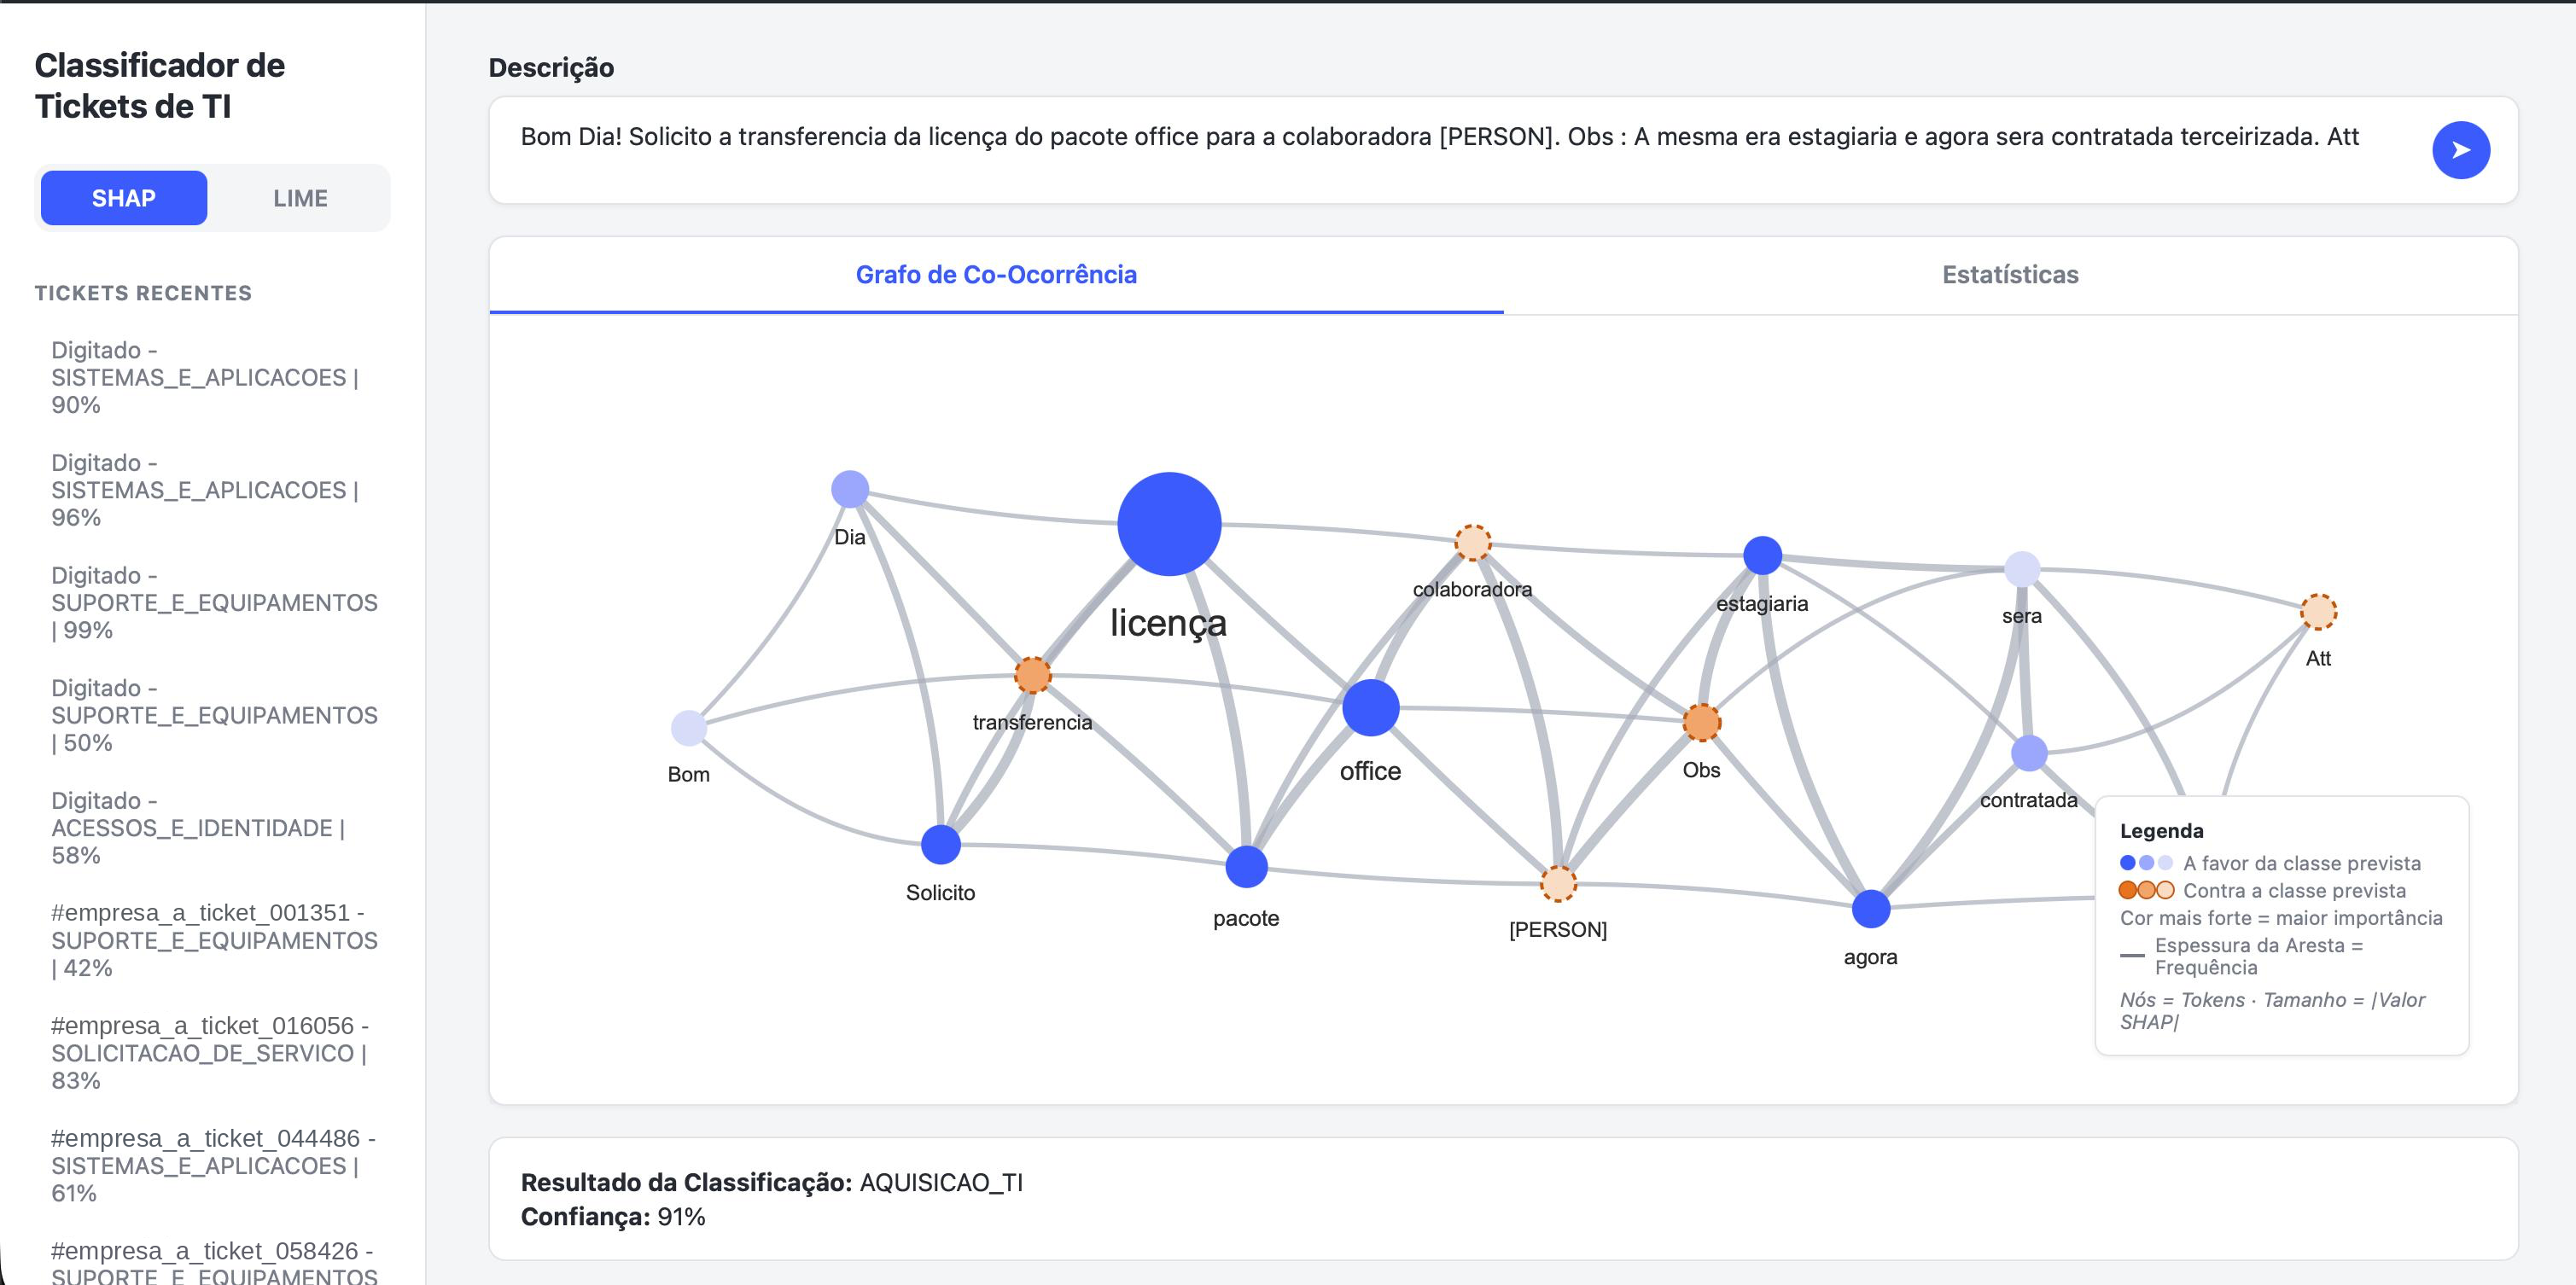
\includegraphics[width=\textwidth]{imagens/grafo_caso1_empresa_b_001118.png}\\[8pt]
    \textbf{(b) LIME}\\[2pt]
    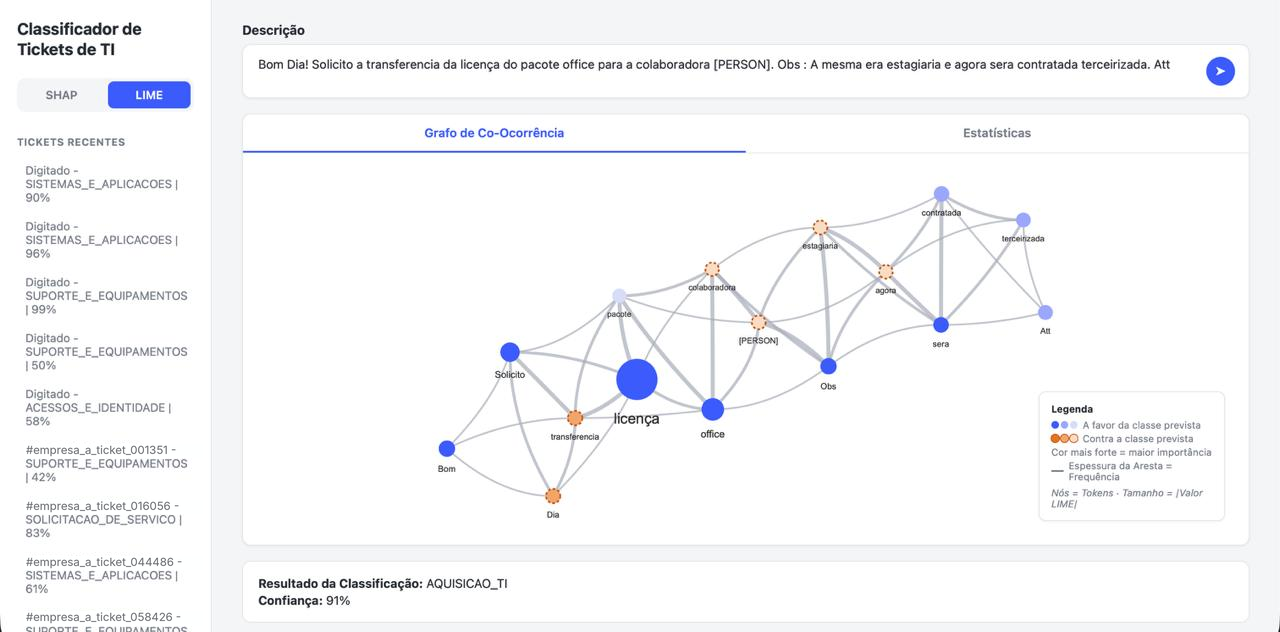
\includegraphics[width=\textwidth]{imagens/grafo_caso1_empresa_b_001118_lime.png}
    \legend{Fonte: Elaborado pelos autores.}
\end{figure}

No caso 2, o chamado tem uma única frase, sobre a instalação de duas impressoras, e a categoria real é OUTROS; o modelo previu SUPORTE\_E\_EQUIPAMENTOS com confiança de 0,42. O grafo tem apenas 4 nós. A palavra de maior peso, \textit{Rena}, a marca de uma das impressoras, pesa contra a classe prevista (SHAP de $-$0,248; LIME de $-$0,290), assim como \textit{impressoras} ($-$0,101 e $-$0,077), enquanto o marcador de anonimização \textit{[PERSON]} pesa a favor (0,124 e 0,144). A explicação mostra que a decisão se apoiou em muito pouca evidência e que um marcador de anonimização influenciou a previsão, o que um analista pode questionar. Vale notar que, na taxonomia harmonizada, os chamados de impressora da Empresa A (PRINT\_FAX) pertencem a SUPORTE\_E\_EQUIPAMENTOS, e a classe OUTROS vem apenas da categoria CORE\_OTHER. Assim, a previsão do modelo está de acordo com a taxonomia, e o erro pode refletir um rótulo original pouco informativo; a explicação ajuda justamente a levantar essa dúvida.

\begin{figure}[H]
    \caption{Grafo de co-ocorrência do caso 2 (empresa\_a\_ticket\_001351): (a) pesos SHAP; (b) pesos LIME}
    \label{fig:grafo_caso2}
    \centering
    \textbf{(a) SHAP}\\[2pt]
    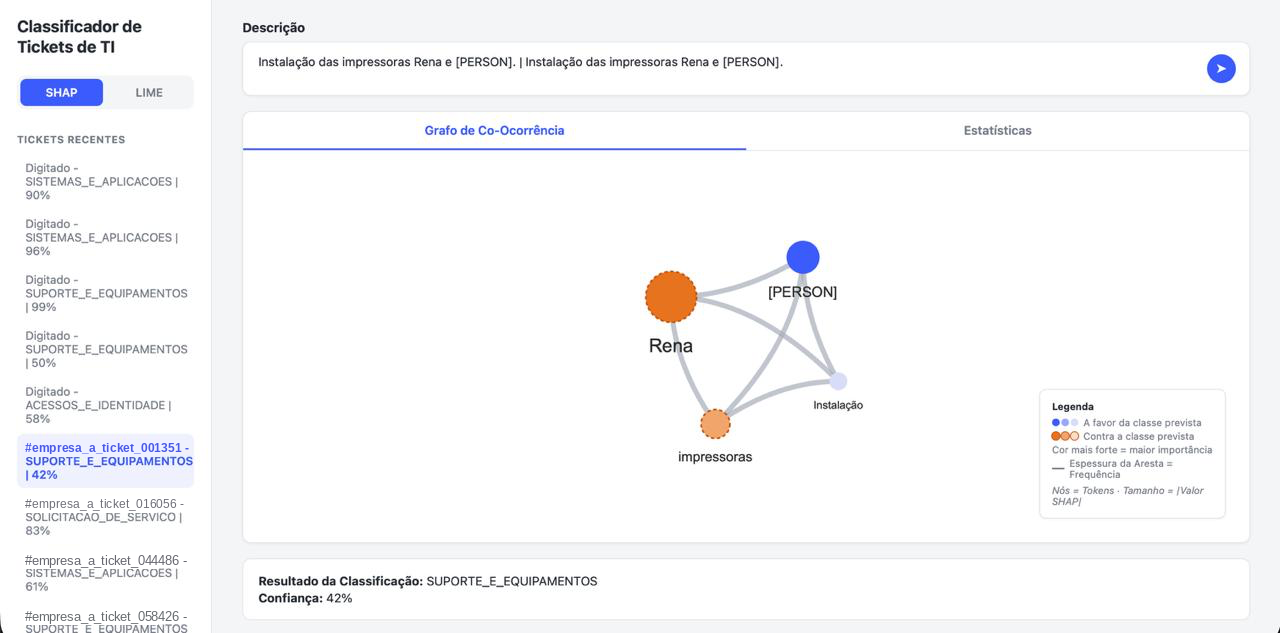
\includegraphics[width=\textwidth]{imagens/grafo_caso2_empresa_a_001351.png}\\[8pt]
    \textbf{(b) LIME}\\[2pt]
    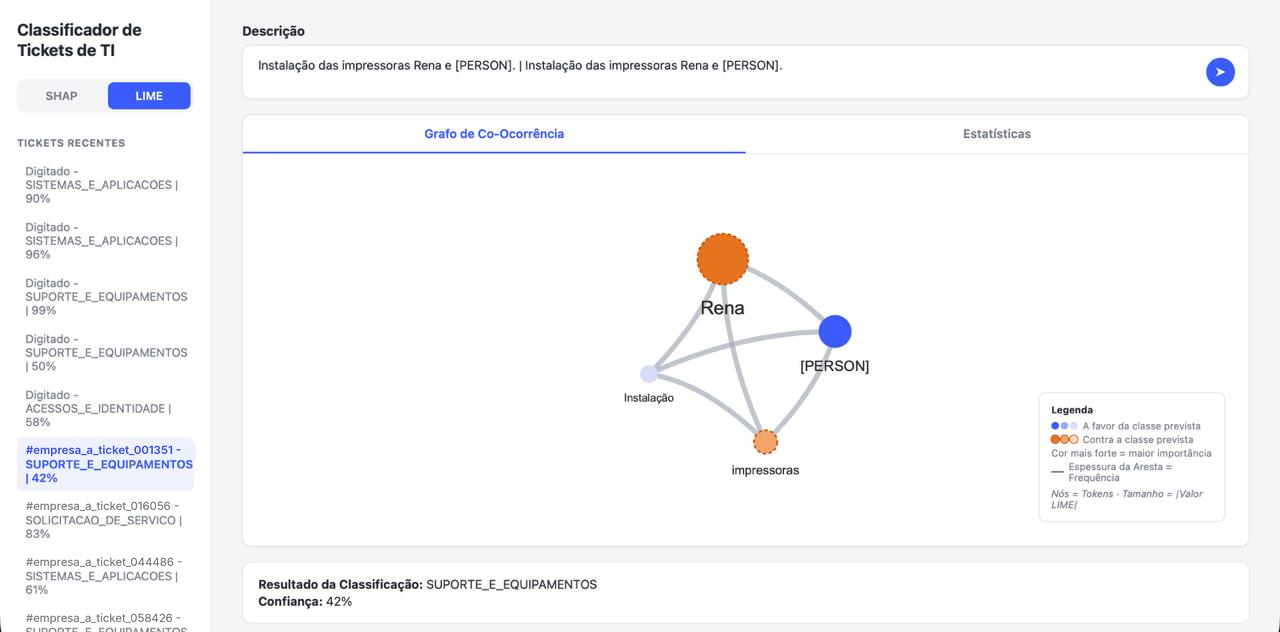
\includegraphics[width=\textwidth]{imagens/grafo_caso2_empresa_a_001351_lime.png}
    \legend{Fonte: Elaborado pelos autores.}
\end{figure}

No caso 3, o chamado pede a limpeza de um \textit{rack}. Os dois métodos concordam na palavra de maior peso, \textit{Favor} (SHAP de 0,322; LIME de 0,346), típica de um pedido de serviço. Nas demais palavras, porém, divergem: \textit{limpeza} tem peso de 0,165 no SHAP e de apenas 0,002 no LIME. O grafo, construído com os pesos do SHAP, e o do LIME, portanto, destacam conjuntos diferentes de palavras além da primeira, o que o analista pode verificar alternando o método na interface.

\begin{figure}[H]
    \caption{Grafo de co-ocorrência do caso 3 (empresa\_a\_ticket\_016056): (a) pesos SHAP; (b) pesos LIME}
    \label{fig:grafo_caso3}
    \centering
    \textbf{(a) SHAP}\\[2pt]
    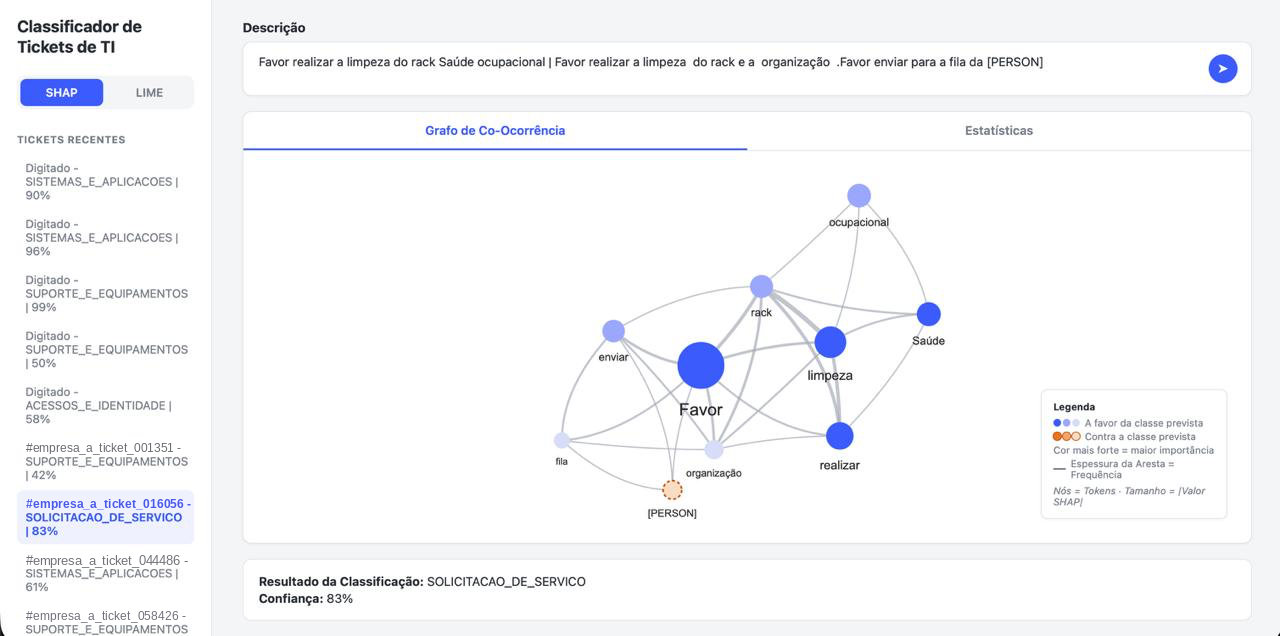
\includegraphics[width=\textwidth]{imagens/grafo_caso3_empresa_a_016056.png}\\[8pt]
    \textbf{(b) LIME}\\[2pt]
    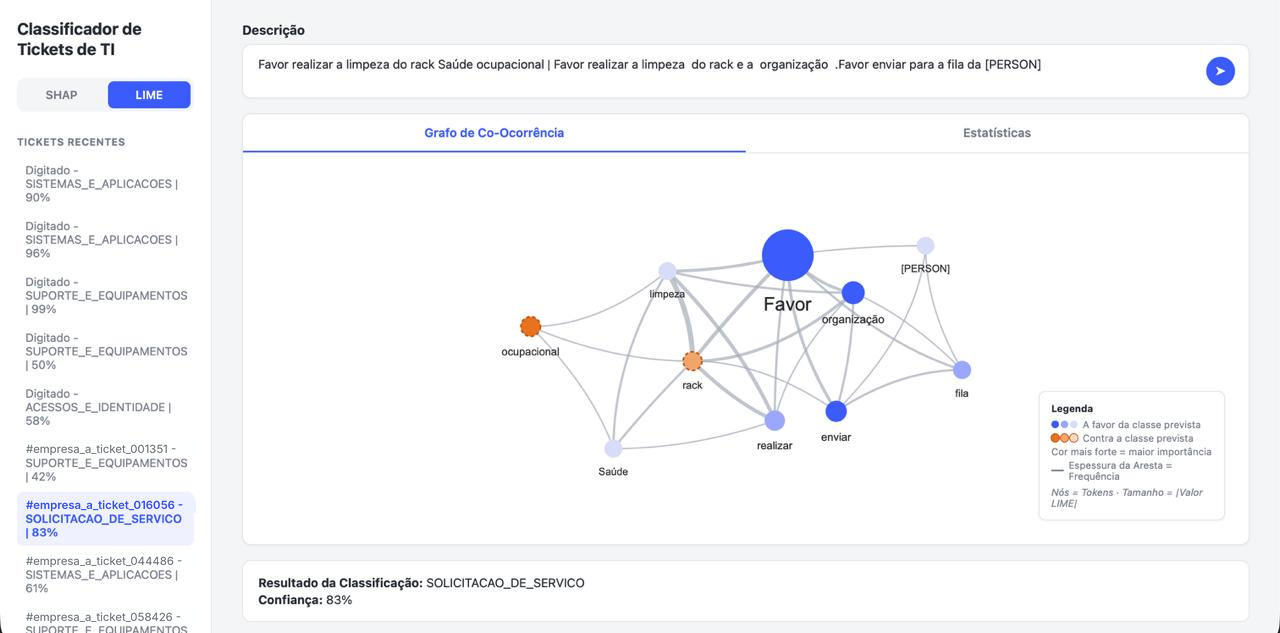
\includegraphics[width=\textwidth]{imagens/grafo_caso3_empresa_a_016056_lime.png}
    \legend{Fonte: Elaborado pelos autores.}
\end{figure}

\subsection{Análise crítica e comparação}
\textbf{Classificação.} O BERTimbau superou o \textit{baseline} SVM em 3,7 pontos percentuais de F1-macro, abaixo da meta de 5 pontos estabelecida inicialmente. Os dados mostram que o ganho existe, mas não que ele atinja o critério, pois o intervalo de confiança inclui o 5. O ganho vem da revocação e se concentra em poucas classes (SOFTWARE e SOLICITACAO\_DE\_SERVICO, além de duas classes pequenas), enquanto na maior classe os dois modelos empatam. Há ainda dois cuidados de leitura: o resultado na Empresa B é pouco informativo, pois seus chamados formam poucos grupos de texto, e na validação um único texto repetido 491 vezes inflaria a diferença para 11,9 pontos. Por isso, o resultado mais seguro é o do teste, com os grupos de texto reamostrados juntos. Os valores de F1-macro de outros trabalhos de classificação de chamados (Seção~\ref{sec:trabalhos_relacionados}) não são diretamente comparáveis com os deste, pois as bases, as categorias e os cenários diferem.
 
\textbf{Fidelidade.} O SHAP e o LIME têm fidelidade bem acima do acaso, e a comparação chamado a chamado não distingue os métodos na \textit{comprehensiveness} nem na \textit{sufficiency}. Só no Tau-LOO há diferença, a favor do LIME (diferença média de $-$0,051 para o SHAP, com intervalo que exclui o zero). Isso difere do que se poderia esperar de um método com garantias teóricas como o SHAP, mas uma diferença em uma das três medidas não basta para afirmar que o LIME seja mais fiel.
 
\textbf{Estabilidade.} Esperava-se que o SHAP fosse mais estável que o LIME, que depende de amostragem aleatória \cite{ribeiro2016}. Neste trabalho, o SHAP é perfeitamente estável quando calculado de forma exata, o que ocorre em textos curtos (até 10 palavras por campo). Nos 9 chamados em que foi estimado por amostragem, com orçamento de 2.000 consultas, ficou mais estável que o LIME no Jaccard (0,634 contra 0,546) e no Spearman (0,861 contra 0,706), mas o LIME manteve a mesma palavra no topo com mais frequência (93\% dos pares de repetições, contra 83\%). O resultado depende do orçamento: com 500 consultas, o SHAP estimado era menos estável que o LIME nas três medidas, e a estabilidade continuou crescendo com 5.000 (Tabela~\ref{tab:res_orcamento}). O orçamento é, portanto, um parâmetro que troca tempo de processamento por estabilidade. A amostra de 12 chamados é pequena e não houve teste estatístico, então as conclusões são indicativas.
 
\textbf{Concordância.} Os dois métodos concordam bem acima do acaso (a mesma palavra no topo em 69\% dos chamados), mas a concordância cai com o tamanho do texto. Assim, em chamados longos, a escolha do método muda de forma relevante quais palavras o analista vê como importantes.
 
\textbf{Grafo.} Nos três casos aplicados, a rastreabilidade se cumpriu: cada nó e cada aresta puderam ser levados ao chamado e aos pesos do SHAP e do LIME. Os casos também mostraram o uso prático da explicação: no caso 2, ela expôs que um erro do modelo se apoiou em muito pouca evidência e em um marcador de anonimização, e no caso 3, que os dois métodos concordam na palavra de maior peso, mas destacam palavras diferentes depois dela. A limitação é que três casos, escolhidos para ilustrar situações diferentes, mostram que o grafo é rastreável, mas não que ele melhore a decisão de um analista.

\subsection{Discussão}
A hipótese de pesquisa (Seção~\ref{sec:hipotese_pesquisa}) tem duas partes, e os resultados as sustentam de forma diferente. A primeira afirma que o grafo ponderado pelos valores SHAP e LIME contribui para a auditabilidade ao permitir rastrear os termos que levaram à categoria. Essa parte foi sustentada nos termos em que foi definida, a rastreabilidade, nos três casos aplicados. Como a auditabilidade foi medida por rastreabilidade e não em um teste com analistas, o resultado mostra que o caminho da decisão pode ser reconstruído, e não que um analista o reconstrua com facilidade. As outras duas dimensões da definição de auditabilidade (Seção~\ref{subsec:auditabilidade}), a fidelidade e a estabilidade, foram medidas nas explicações do cenário C (Seção~\ref{subsec:res_xai}).
 
A segunda parte afirma que o SHAP e o LIME produzem explicações com fidelidade e estabilidade distintas. Na fidelidade, a diferença é pequena e só aparece em uma das três medidas, a favor do LIME. Na estabilidade, a diferença depende de como o SHAP é calculado: ele é perfeitamente estável quando exato e, quando estimado por amostragem com 2.000 consultas, mais estável que o LIME no Jaccard e no Spearman, mas menos na mesma palavra no topo. A parte é, portanto, sustentada de forma condicional, e o resultado não sustenta a ideia de que um método seja melhor em todos os casos.
 
Em relação aos objetivos específicos, o ganho do BERTimbau sobre o \textit{baseline} foi analisado (3,7 pontos, abaixo do critério de 5), e SHAP e LIME foram comparados em fidelidade, estabilidade e concordância. Quanto à consistência semântica das explicações, o objetivo foi atendido apenas de forma qualitativa, nos casos: no caso 1, as palavras de maior peso (\textit{licença} e \textit{office}) são o vocabulário esperado para a classe, e no caso 2 a explicação mostra uma previsão apoiada em muito pouca evidência. \citeonline{razma2026} observam, em exemplos de LIME, que o BERT atribui pesos mais contextuais aos termos do chamado do que a regressão logística; os casos analisados aqui mostram que isso ocorre em alguns chamados, mas não em todos.
 
Para a prática de suporte, os resultados sugerem que o grafo é mais útil como ferramenta de auditoria dos erros e das previsões de baixa confiança, como no caso 2, do que como justificativa de todos os acertos. Por fim, os resultados valem para os dados e a configuração usados (duas empresas, um treinamento, uma amostra de 98 chamados), e as limitações descritas no Capítulo~\ref{cap:conclusao} delimitam o alcance das conclusões.

% ===============================================================
% CAPÍTULO 4 - CONCLUSÃO
% ===============================================================
\chapter{Conclusão}
\label{cap:conclusao}

\section{Retomada do problema e dos objetivos}
Este trabalho partiu de um problema: classificadores baseados em \textit{transformers} acertam bem a categoria de um chamado de TI, mas não mostram por que a escolheram, o que dificulta a auditoria de suas decisões. A pergunta de pesquisa foi como se comparam o SHAP e o LIME quanto à fidelidade e à estabilidade das explicações de um classificador BERTimbau e de que forma um grafo de co-ocorrência contribui para tornar o processo de classificação auditável.

Para respondê-la, os chamados de duas empresas (53.279 chamados, em 11 categorias) foram usados para treinar um \textit{baseline} SVM com TF-IDF e ajustar o BERTimbau, e as decisões do BERTimbau foram explicadas por SHAP e LIME e representadas em um grafo. Os resultados, por objetivo específico, foram os seguintes.

\begin{enumerate}
    \item \textbf{Ganho do BERTimbau sobre o \textit{baseline}.} O objetivo foi atendido: o BERTimbau obteve F1-macro de 0,628 contra 0,591 do SVM, uma diferença de 3,7 pontos percentuais, abaixo da meta de 5 pontos estabelecida inicialmente. O ganho existe, mas os dados não mostram que atinja o critério, e ele se concentra em poucas classes.

    \item \textbf{Comparação entre SHAP e LIME.} O objetivo foi atendido: em 98 chamados, os dois métodos tiveram fidelidade bem acima do acaso e não se distinguiram na \textit{comprehensiveness} nem na \textit{sufficiency}; só o Tau-LOO foi maior no LIME. Na estabilidade, o SHAP foi perfeito quando calculado de forma exata e, quando estimado por amostragem com 2.000 consultas, mais estável que o LIME no Jaccard e no Spearman, mas menos na mesma palavra no topo. Os dois apontaram a mesma palavra no topo em 69\% dos chamados, e a concordância caiu com o tamanho do texto.

    \item \textbf{Auditabilidade pelo grafo.} O objetivo foi atendido nos três casos aplicados: cada nó e cada aresta puderam ser levados ao chamado e aos pesos do SHAP e do LIME, o que corresponde à auditabilidade nos termos em que foi definida, a rastreabilidade. Não se mediu, porém, se analistas conseguem acompanhar a decisão a partir do grafo.

    \item \textbf{Consistência semântica.} O objetivo foi atendido apenas de forma qualitativa, nos casos: em um deles, as palavras de maior peso são o vocabulário esperado para a classe, e em outro a explicação expôs uma previsão apoiada em muito pouca evidência.
\end{enumerate}

Assim, a hipótese de pesquisa foi sustentada na parte da rastreabilidade e, na parte da comparação entre os métodos, de forma condicional: nenhum dos dois foi melhor em todas as medidas.

\section{Contribuições para a Computação}
As contribuições deste trabalho para a área são as seguintes.
 
\begin{itemize}
    \item \textbf{Comparação empírica entre SHAP e LIME em chamados de TI em português.} A literatura identificada não traz essa comparação para um BERT \textit{fine-tuned} em chamados de suporte em português brasileiro (Seções~\ref{sec:metodologia_pesquisa_bib} e~\ref{subsec:sintese_lacunas}). Os resultados mostram que a vantagem de estabilidade atribuída ao SHAP depende de como ele é calculado, e que a escolha do método importa mais em textos longos.
 
    \item \textbf{Metodologia de avaliação das explicações.} O trabalho reúne, em um mesmo procedimento, medidas de fidelidade, estabilidade e concordância, cada uma comparada ao valor esperado ao acaso, com intervalos de confiança por \textit{bootstrap} pareado. O procedimento pode ser reaplicado a outros classificadores de texto.
 
    \item \textbf{Grafo de co-ocorrência com pesos SHAP e LIME como camada de auditabilidade.} O grafo liga cada decisão às palavras do chamado, à janela de co-ocorrência e aos pesos dos dois métodos, e foi implementado em uma interface \textit{web} que serve de prova de conceito.
 
    \item \textbf{Evidência sobre o BERTimbau frente a um \textit{baseline} clássico.} O trabalho mede o ganho do modelo neural em chamados reais de duas empresas, com a divisão dos dados agrupada pelo texto do chamado, de modo que textos repetidos não vazem entre treino e teste, e mostra como textos muito repetidos podem inflar a diferença entre os modelos.
\end{itemize}

\section{Limitações e trabalhos futuros}
Este trabalho tem limitações que delimitam o alcance de seus resultados.

Quanto aos dados, os chamados vêm de apenas duas empresas do setor farmacêutico, e a Empresa A reúne 86\% do conjunto de teste. Os chamados da Empresa B cobrem um único mês (abril de 2026) e têm muitos textos repetidos: os 716 chamados de teste dessa empresa formam apenas 337 grupos de texto, de modo que o resultado na Empresa B traz menos informação do que o número de chamados sugere. A classe OUTROS tem apenas 12 chamados no teste e nenhum foi acertado, então o desempenho nela não pôde ser avaliado de forma conclusiva. As categorias das duas empresas foram harmonizadas em uma taxonomia única, e os resultados dependem dessa escolha. Além disso, a varredura de sanidade da anonimização encontrou, na base final, 24 ocorrências residuais de padrão telefônico rotulado na descrição (0 no resumo), que podem incluir falsos positivos; a anonimização, portanto, não pode ser considerada perfeita.

Além disso, dos 189.909 chamados da Empresa A que restaram após a limpeza, 143.325 não estavam em português e foram descartados pelo filtro de idioma, e não traduzidos; traduzi-los poderia ampliar a base, ao custo de introduzir ruído de tradução no vocabulário técnico. Uma amostra de 30 chamados mantidos e 30 descartados foi revisada manualmente, julgando o pedido do chamado e não os campos fixos do formulário: o filtro acertou os 30 mantidos e 25 dos 30 descartados (55 de 60). Os cinco desacordos são chamados cujo pedido está em português, em geral um título ou uma frase curta dentro de um formulário em inglês, e que o filtro descartou. Nenhum chamado em inglês foi mantido. % CONFERIDO: amostra de 60 em language_filter_review_sample.csv; 30/30 mantidos e 25/30 descartados. Os 5 erros sao descarte de pedido em portugues.

Quanto à classificação, os resultados vêm de um único treinamento do BERTimbau (semente 42), sem repetição com outras sementes. A tentativa de melhoria com pesos de classe (Seção~\ref{subsec:res_melhoria}) não superou a referência e foi relatada como complementar, pois o escopo escolhido para ela foi definido depois de observados resultados de teste. O intervalo de confiança da diferença para o \textit{baseline} SVM (de 1,0 a 6,7 pontos) inclui tanto ganhos pequenos quanto o critério de 5 pontos, e cerca de 10,2\% dos pares de texto ultrapassam o limite de 256 \textit{tokens}, de modo que o trecho excedente não chega ao modelo. A confiança exibida pela interface é a probabilidade máxima da \textit{softmax} e não foi calibrada.

Quanto à escolha do modelo, o trabalho usou o BERTimbau, um modelo de 2020, e não avaliou modelos generalistas mais recentes, os LLMs (\textit{Large Language Models} -- Modelos de Linguagem de Grande Porte), nem abordagens com recuperação de contexto (RAG, \textit{Retrieval-Augmented Generation} -- Geração Aumentada por Recuperação) ou explicações em texto geradas pelo próprio modelo, como as de CoT (\textit{Chain-of-Thought} -- Cadeia de Raciocínio). O BERTimbau foi mantido por ser específico para o português e por permitir calcular, em máquinas locais, as centenas de consultas ao modelo que o SHAP e o LIME exigem por explicação; com um LLM, esse custo seria bem maior. Já as explicações em texto de um LLM teriam de ter sua fidelidade ao processo de decisão avaliada com medidas como as usadas aqui.

Quanto às explicações, o SHAP e o LIME foram avaliados em uma amostra de 98 chamados, e a estabilidade em apenas 12 deles, explicados 5 vezes cada e escolhidos entre os que têm ao menos oito palavras distintas, o que impede estender esse resultado a chamados curtos. Em 79 dos 166 campos explicados, o SHAP foi estimado por amostragem, com orçamento de 2.000 consultas, enquanto o LIME usou 500 amostras, de modo que a comparação de estabilidade não é entre métodos de mesmo custo; o teste com 500, 2.000 e 5.000 consultas mostrou que a estabilidade do SHAP aumenta com o orçamento. Em alguns chamados, o modelo linear local do LIME ajusta pouco o comportamento do classificador (o $R^2$ local teve mediana de 0,68 e mínimo de 0,11). Além disso, a \textit{comprehensiveness} e a \textit{sufficiency} foram implementadas pelos autores, seguindo a definição de \citeonline{attanasio2023}, e o Tau-LOO usa o tau-b de \texttt{scipy.stats.kendalltau}; por isso esses valores podem não ser diretamente comparáveis aos de estudos que usam a biblioteca \textit{ferret}.  A fidelidade e a estabilidade não foram calculadas para o SVM, que é interpretável por construção, e a comparação das explicações entre os cenários A e B fica como trabalho futuro.

Quanto ao grafo, a auditabilidade foi avaliada pela rastreabilidade, em casos aplicados, e não em um teste com analistas de TI. O trabalho, portanto, mostra que cada nó e cada aresta podem ser levados de volta ao chamado, mas não que analistas conseguem, na prática, acompanhar a decisão do classificador a partir do grafo.

Como trabalhos futuros, sugerem-se: (i) repetir o treinamento com outras sementes e incluir chamados de outras empresas e de períodos mais longos; (ii) explicar uma amostra maior de chamados, com mais amostras e consultas por explicação, para medir a estabilidade com mais precisão; (iii) avaliar o grafo em um teste com analistas de TI; (iv) comparar o grafo ponderado por SHAP e por LIME com outras formas de apresentar as explicações; e (v) comparar o BERTimbau com modelos generalistas mais recentes e avaliar abordagens com RAG e explicações por CoT.

% ---------------------------------------------------------------
% ELEMENTOS PÓS-TEXTUAIS
% ---------------------------------------------------------------
\postextual

% ===============================================================
% CAPÍTULO 4 - REFERÊNCIAS BIBLIOGRÁFICAS
% ===============================================================
\bibliography{bibliografia}
\bibliographystyle{abntex2-alf}
% ---------------------------------------------------------------
% APÊNDICES (se necessário)
% ---------------------------------------------------------------
\begin{apendicesenv}
\partapendices

\chapter{Cronograma de atividades}
\label{ap:cronograma}

O cronograma a seguir apresenta as fases do Trabalho de Conclusão de Curso II (TCC2), com as datas em que foram concluídas e o status atual.

\begin{table}[htb]
  \centering
  \caption{Cronograma do TCC2, com datas e status}
  \label{tab:cronograma}
  \small
  \begin{tabular}{p{4.2cm}p{4.6cm}p{3.6cm}}
    \toprule
    Fase & Período & Status \\
    \midrule
    1. Dados e modelo & setembro a 05/10/2026 & Concluída (modelo final treinado de 04/10 a 05/10) \\
    2. XAI e grafo & outubro a 01/11/2026 & Concluída (rodada oficial do SHAP e do LIME em 01/11) \\
    3. Sistema e interface & até 05/11/2026 & Concluída (prova de conceito funcionando em 05/11) \\
    4. Escrita do documento & 02/11 a 07/11/2026 & Concluída (capítulos 1 a 4 redigidos) \\
    5. Prévia e entrega & 10/11 e 27/11/2026 & Prévia da banca realizada; entrega final agendada\\
    \bottomrule
  \end{tabular}
  \legend{Fonte: Elaborado pelos autores.\\ Nota: Em relação ao plano inicial, a interface passou a ser servida com \textit{Flask}, em vez de \textit{FastAPI}.}
\end{table}

\chapter{Correspondência entre as categorias originais e a taxonomia harmonizada}
\label{ap:correspondencia_categorias}

A Tabela~\ref{tab:correspondencia_categorias} lista as 54 categorias do arquivo de correspondência usado na harmonização (45 da Empresa A e 9 da Empresa B) e a classe da taxonomia harmonizada (Seção~\ref{subsubsec:dataset_finetuning}) a que cada uma foi associada. A classe RECURSOS\_HUMANOS, exclusiva da Empresa B, tem 39 chamados e ficou fora do treino por ter menos de 100 exemplos; por isso o modelo tem 11 classes. O nome de uma empresa que aparecia em uma categoria da Empresa A foi substituído por [ORG].

{\footnotesize\setlength{\tabcolsep}{3pt}
\begin{longtable}{p{5.5cm}p{1.7cm}p{7.5cm}}
  \caption{Correspondência entre as categorias originais e a taxonomia harmonizada}
  \label{tab:correspondencia_categorias} \\
  \toprule
  Classe harmonizada & Empresa & Categoria original \\
  \midrule
  \endfirsthead
  \multicolumn{3}{l}{\textit{(continuação da Tabela~\ref{tab:correspondencia_categorias})}} \\
  \toprule
  Classe harmonizada & Empresa & Categoria original \\
  \midrule
  \endhead
  \midrule
  \multicolumn{3}{r}{\textit{(continua na próxima página)}} \\
  \endfoot
  \bottomrule
  \multicolumn{3}{l}{Fonte: Elaborado pelos autores.} \\
  \endlastfoot
    ACESSOS\_E\_IDENTIDADE & Empresa A & PASSWORD\_RESET \\
     & Empresa A & USER\_MANAGEMENT \\
     & Empresa A & IMCM\_USER\_MANAGEMENT\_REQUESTS \\
     & Empresa A & FILE\_FOLDER \\
     & Empresa A & WORKPLACE\_TOOLS \\
     & Empresa A & WORKSPACEONE \\
     & Empresa A & ISC\_Identity \\
     & Empresa A & ISC\_Access \\
     & Empresa B & RS - Acessos, senhas \& perfis \\
    \midrule
    CONSULTA\_E\_ORIENTACAO & Empresa A & INQUIRY\_HELP \\
    \midrule
    OUTROS & Empresa A & CORE\_OTHER \\
    \midrule
    REDES\_E\_COMUNICACOES & Empresa A & NETWORK \\
     & Empresa A & VOICE\_VIDEO\_MOBILITY \\
     & Empresa A & VIDEO\_CONFERENCING\_STREAMING \\
     & Empresa B & IN - Redes e Comunicações \\
    \midrule
    SERVIDORES & Empresa A & SERVER \\
     & Empresa A & INFRASTRUCTURE \\
     & Empresa A & SMART AWS (Amazon Web Services) \\
     & Empresa B & IN - Administração e Operação de Servidores \\
    \midrule
    SISTEMAS\_E\_APLICACOES & Empresa A & APPLICATIONS \\
     & Empresa A & CS\_IP21 \\
     & Empresa A & IMCM\_DATA\_ISSUE \\
     & Empresa A & IMCM\_DATA\_UPLOAD\_REQUEST \\
     & Empresa A & IMCM\_SYNC\_ISSUE \\
     & Empresa A & INTEGRATION\_[ORG] \\
     & Empresa A & ORDER\_TO\_CASH\_APPLICATIONS \\
     & Empresa A & OUTLOOK\_SKYPE \\
     & Empresa A & OneMES \\
     & Empresa A & OneMES\_History \\
     & Empresa A & PRODUCT\_SUPPLY\_APPLICATIONS \\
     & Empresa A & SAP\_PLATFORM\_SERVICE\_LINE \\
     & Empresa A & SOURCE\_TO\_PAY\_APPLICATIONS \\
     & Empresa A & IMCM\_CONTENT \\
     & Empresa A & BI \\
     & Empresa A & SHAREPOINT \\
     & Empresa A & ACCOUNTING\_APPLICATIONS \\
     & Empresa A & SERVICENOW \\
     & Empresa A & Interface \\
     & Empresa A & WEB\_APPLICATION \\
     & Empresa A & Global\_Data\_Assets \\
     & Empresa A & EVENT\_MANAGEMENT \\
     & Empresa A & BI\_BASIS \\
     & Empresa A & EDM \\
     & Empresa A & DEVOPS\_PLATFORM \\
     & Empresa B & RS-TI-SISTEMA \\
     & Empresa B & IN-TI-SISTEMA \\
    \midrule
    SOFTWARE & Empresa A & SOFTWARE \\
    \midrule
    SOLICITACAO\_DE\_SERVICO & Empresa A & SERVICE\_REQUEST \\
    \midrule
    SUPORTE\_E\_EQUIPAMENTOS & Empresa A & PC\_HARDWARE \\
     & Empresa A & PRINT\_FAX \\
     & Empresa B & Serviços e Suporte TI \\
    \midrule
    AQUISICAO\_TI & Empresa B & Aquisição de TI \\
    \midrule
    CIBERSEGURANCA & Empresa B & RS-TI-SEGINFO-CIBER \\
    \midrule
    RECURSOS\_HUMANOS & Empresa B & RH - Recursos Humanos \\
\end{longtable}
}

\end{apendicesenv}

% ---------------------------------------------------------------
% ANEXOS (se necessário)
% ---------------------------------------------------------------
\begin{anexosenv}
\partanexos

\chapter{Autorização de uso de dados: Empresa A}
\label{an:autorizacao_empresa_a}

Troca de e-mails em que a Empresa A, por meio de sua equipe de suporte de TI, autoriza o uso de chamados de suporte técnico para fins acadêmicos neste trabalho, mediante anonimização dos registros. Nomes, endereços de e-mail e assinaturas dos participantes, assim como o nome da plataforma interna da empresa, foram ocultados, mantendo-se a data, o assunto e o conteúdo da conversa. As mensagens aparecem em ordem cronológica: o pedido dos autores (Figura~\ref{fig:autorizacao_empresa_a_1}) e a autorização da empresa (Figura~\ref{fig:autorizacao_empresa_a_2}).

\begin{figure}[H]
    \caption{Autorização de uso de dados concedida pela Empresa A (1 de 2): pedido}
    \label{fig:autorizacao_empresa_a_1}
    \centering
    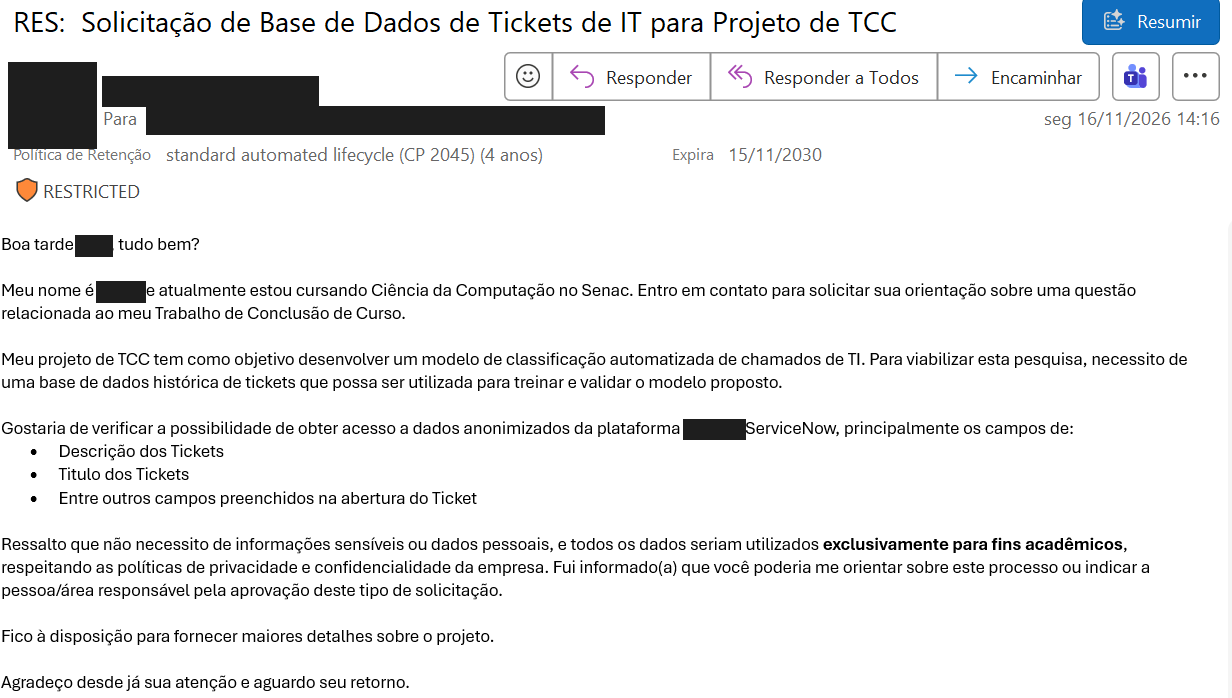
\includegraphics[width=0.9\textwidth]{imagens/autorizacao_empresa_a_1.png}
    \legend{Fonte: Correspondência recebida pelos autores (2026).}
\end{figure}

\begin{figure}[H]
    \caption{Autorização de uso de dados concedida pela Empresa A (2 de 2): autorização}
    \label{fig:autorizacao_empresa_a_2}
    \centering
    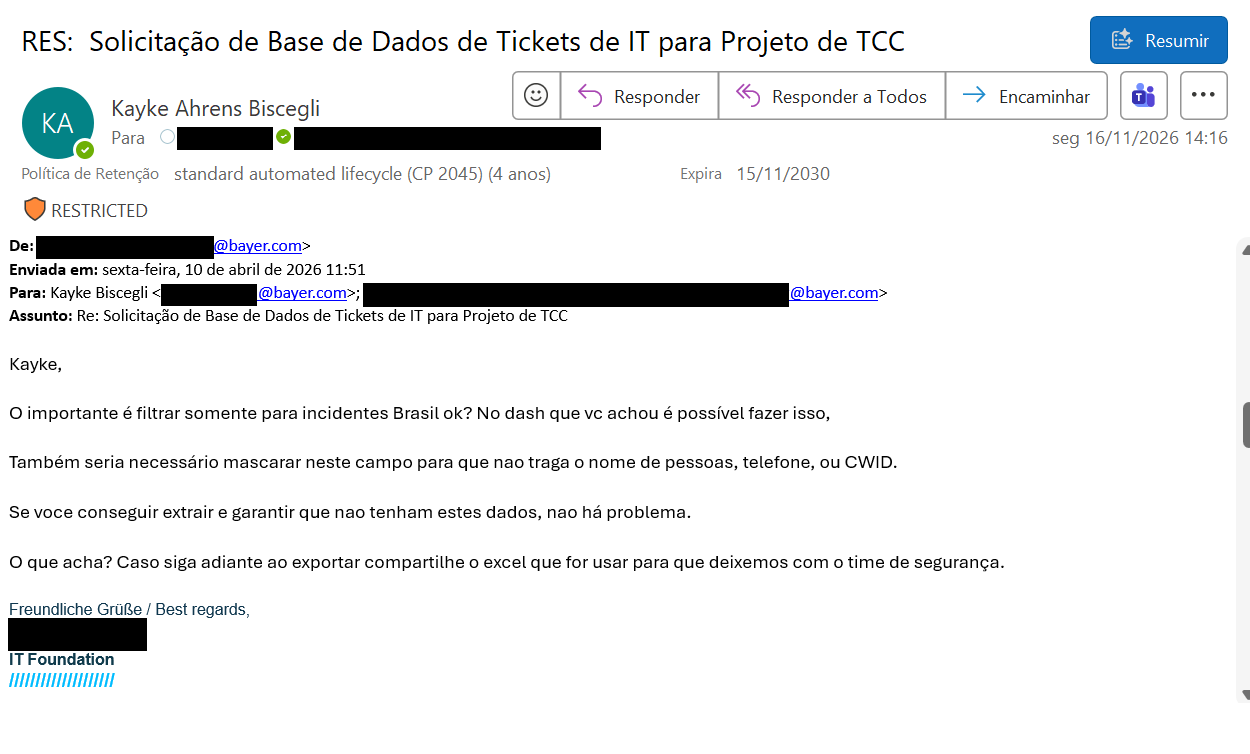
\includegraphics[width=0.9\textwidth]{imagens/autorizacao_empresa_a_2.png}
    \legend{Fonte: Correspondência recebida pelos autores (2026).}
\end{figure}

\chapter{Autorização de uso de dados: Empresa B}
\label{an:autorizacao_empresa_b}

Troca de e-mails em que a Empresa B, por meio de sua equipe de suporte de TI e do prestador do serviço, concorda em compartilhar a base de chamados de suporte técnico para fins acadêmicos neste trabalho. Nomes, endereços de e-mail, telefones e assinaturas dos participantes foram ocultados, mantendo-se a data, o assunto e o conteúdo da conversa. As mensagens aparecem em ordem cronológica: o pedido dos autores e a concordância da empresa (Figura~\ref{fig:autorizacao_empresa_b_1}) e o envio da base de chamados (Figura~\ref{fig:autorizacao_empresa_b_2}).

\begin{figure}[H]
    \caption{Autorização de uso de dados concedida pela Empresa B (1 de 2): pedido e concordância}
    \label{fig:autorizacao_empresa_b_1}
    \centering
    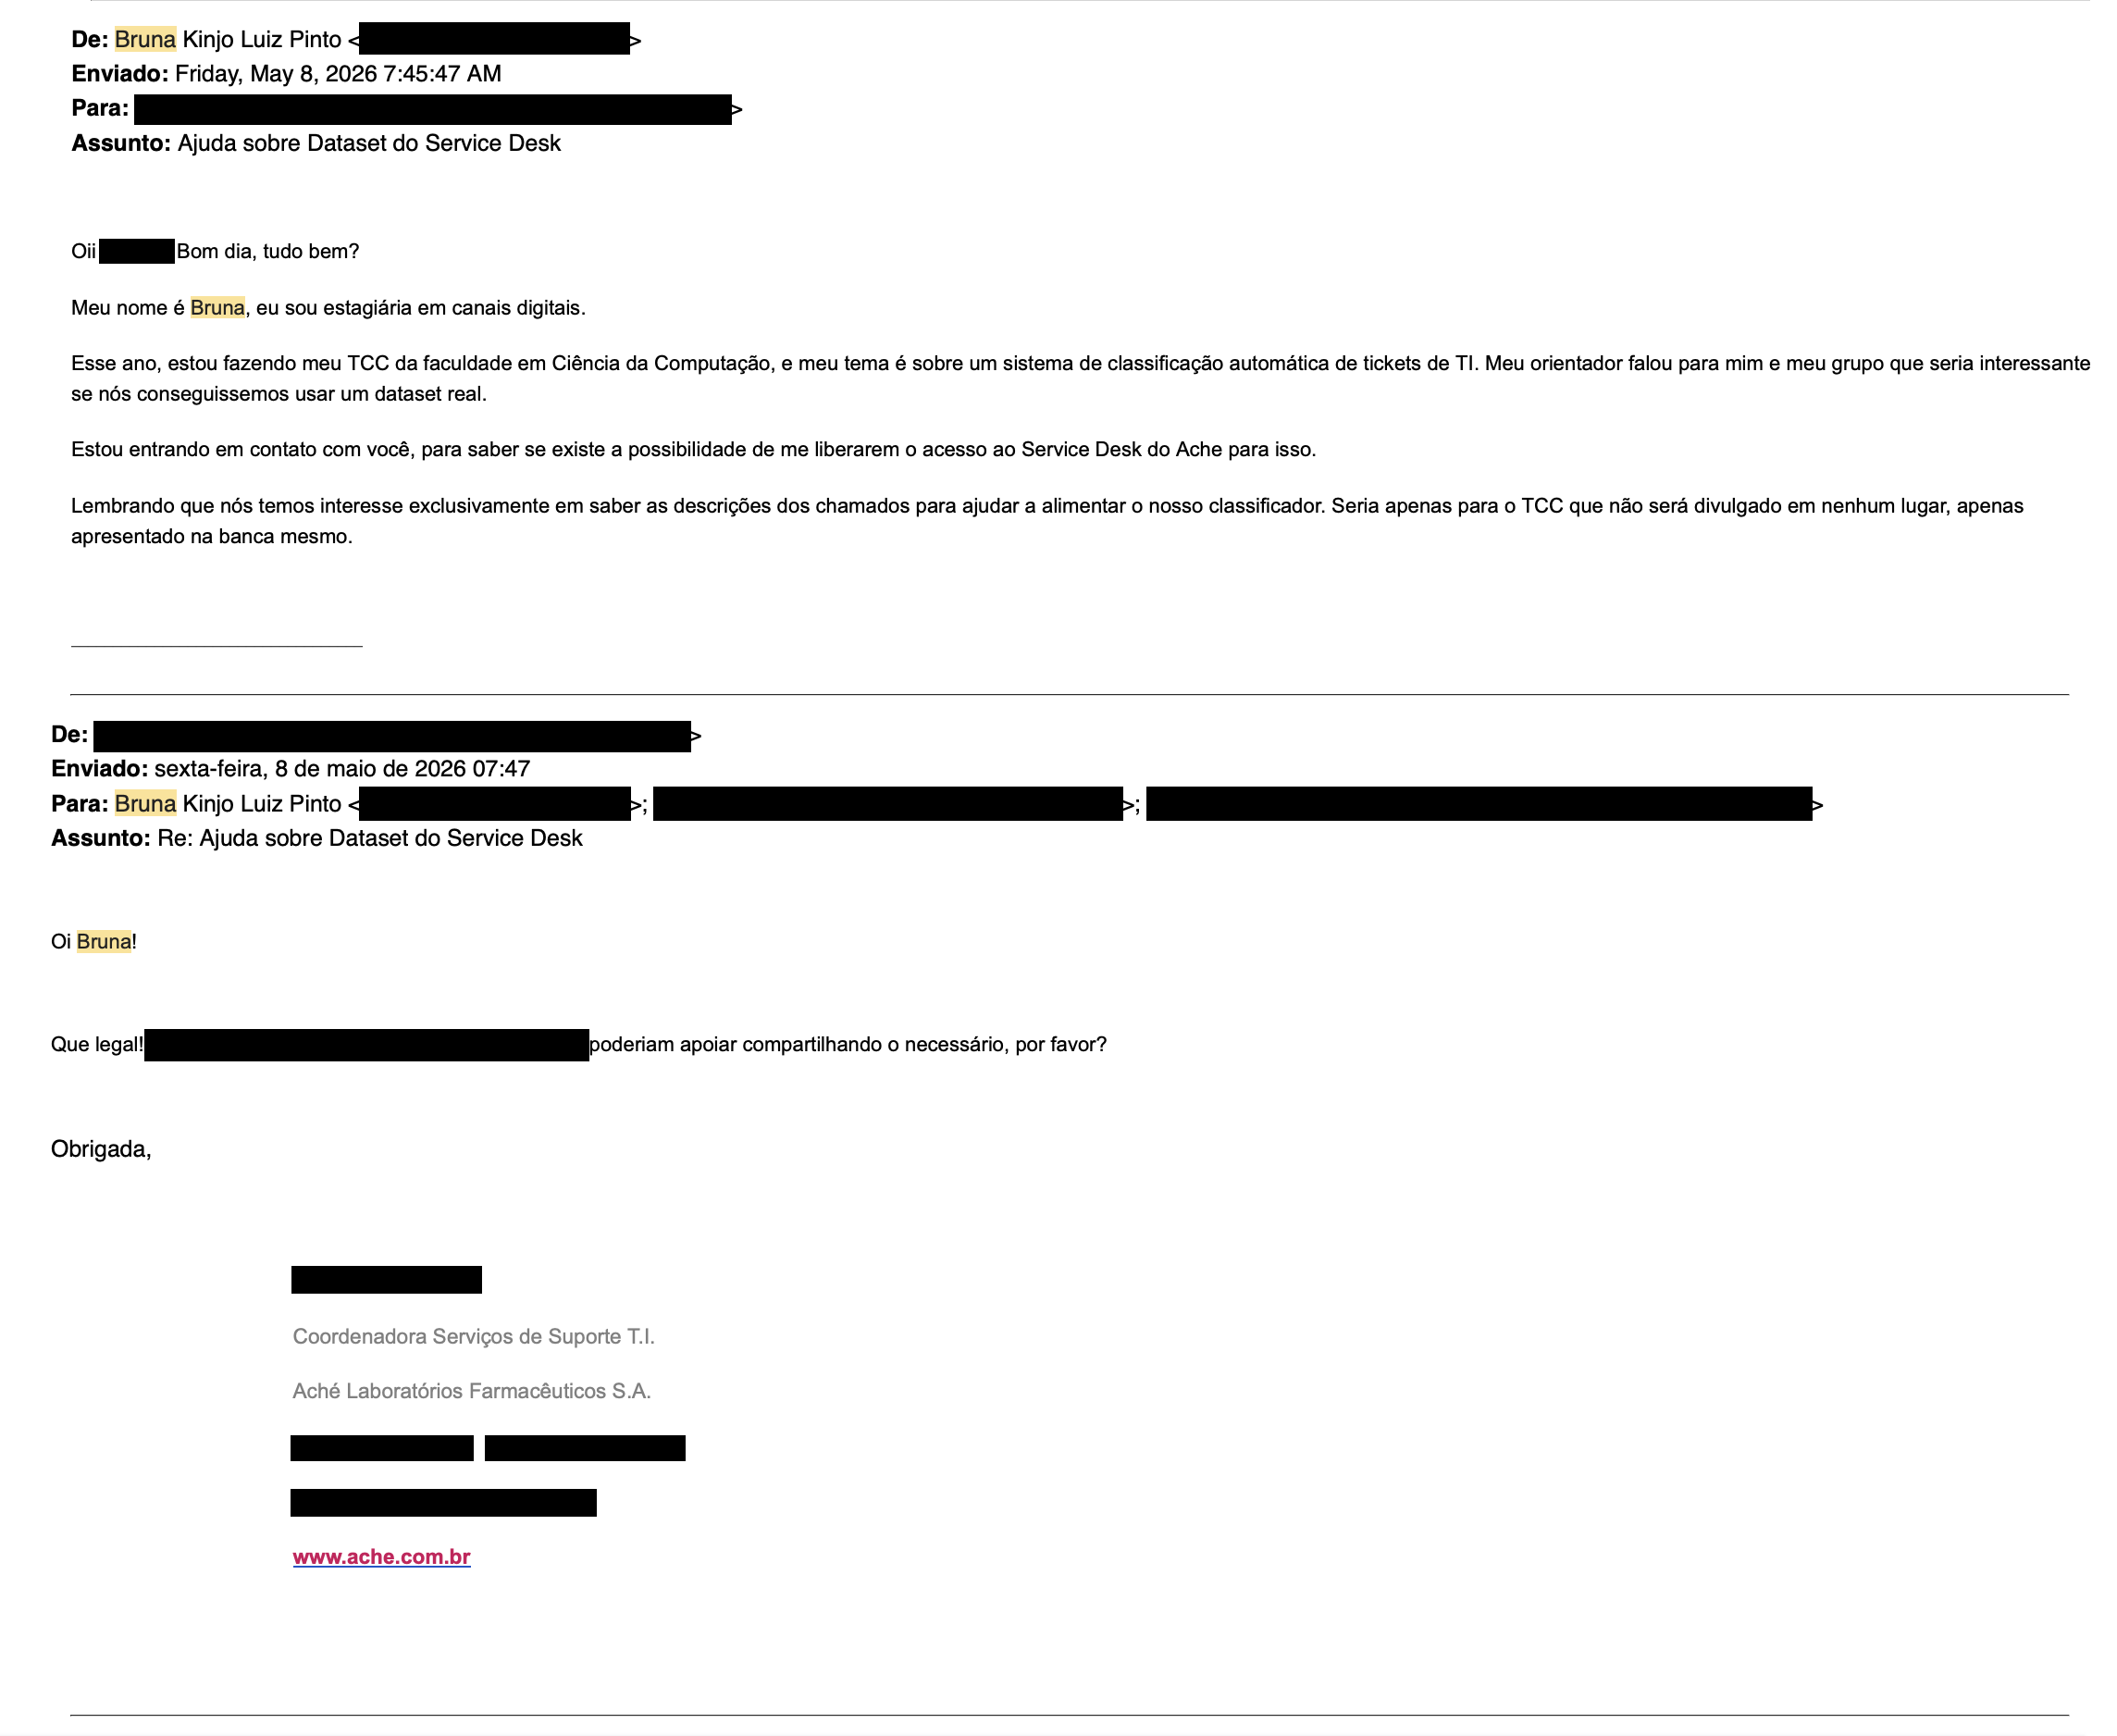
\includegraphics[width=0.9\textwidth]{imagens/autorizacao_empresa_b_1.png}
    \legend{Fonte: Correspondência recebida pelos autores (2026).}
\end{figure}

\begin{figure}[H]
    \caption{Autorização de uso de dados concedida pela Empresa B (2 de 2): acompanhamento e envio da base}
    \label{fig:autorizacao_empresa_b_2}
    \centering
    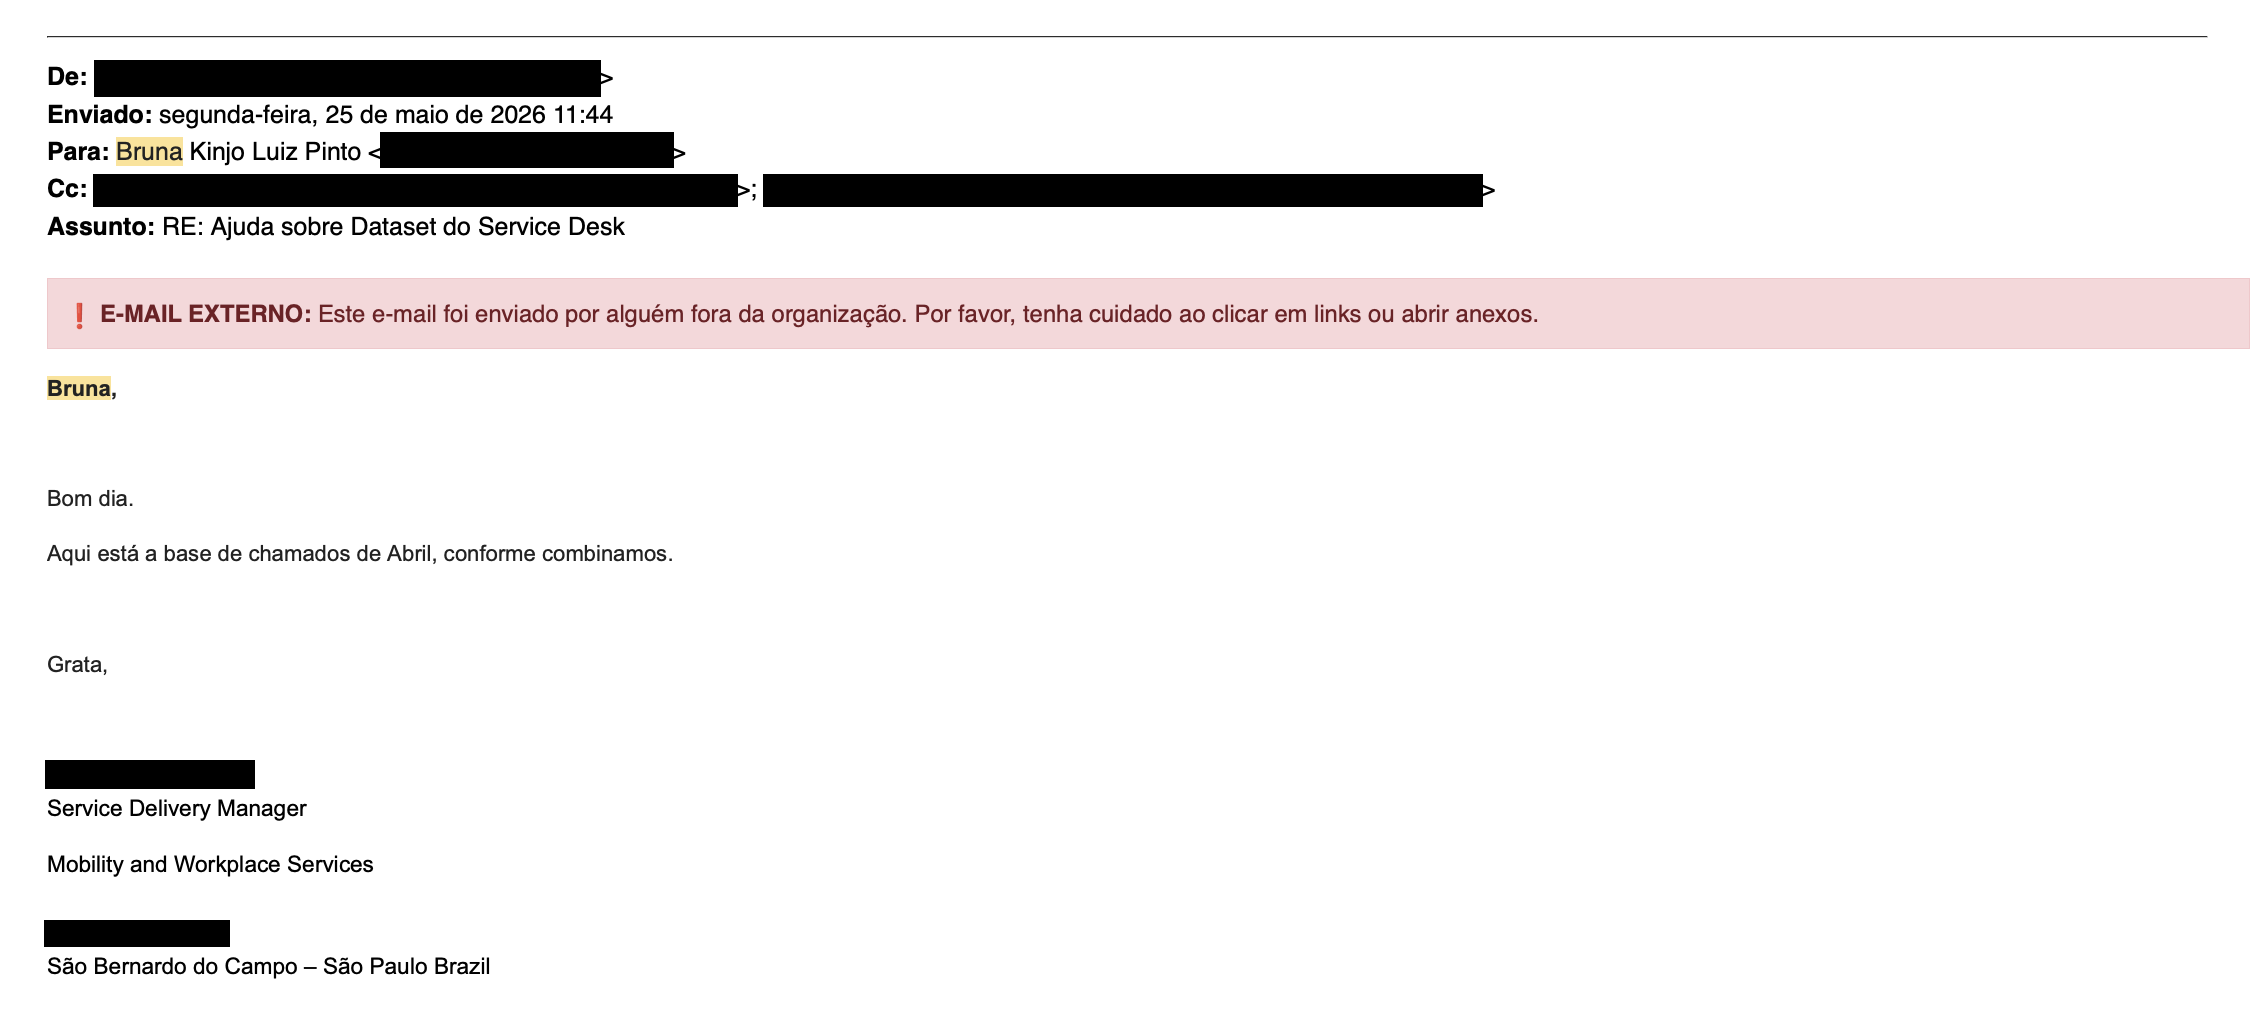
\includegraphics[width=0.9\textwidth,height=0.75\textheight,keepaspectratio]{imagens/autorizacao_empresa_b_2.png}
    \legend{Fonte: Correspondência recebida pelos autores (2026).}
\end{figure}

\end{anexosenv}
% ---------------------------------------------------------------
% ANEXOS
% ---------------------------------------------------------------



\end{document}